%!TeX spellcheck=en_US
\documentclass[11pt,
               a4paper,
               bibtotoc,
               idxtotoc,
               headsepline,
               footsepline,
               footexclude,
               BCOR12mm,
               DIV13,
               openany,   % using this removes blank pages around part / chapter starts.
%               oneside    % include this if you have to print only one page per sheet of paper.
               ]
               {scrbook}

%%% SETTINGS

% no word wrapping
%\righthyphenmin=62
%\lefthyphenmin=62
% fewer hyphens
\usepackage{microtype}

% german symbols
\usepackage[utf8]{inputenc}

% strikethrough by \sout
\usepackage[normalem]{ulem}

% insert graphics
\usepackage{graphicx}
% more flexible figures e.g. graphics with captions beside them
\usepackage{floatrow}
% more flexible captions.
% Use \captionsetup{options} to configure,
% use it in an environment for local setup
\usepackage{caption}
% subfigures (see template):
\usepackage{subcaption}

% more control of enumerations and itemizations
\usepackage{enumitem}
% less space between items
\setlist[itemize]{itemsep=0cm}
\setlist[enumerate]{itemsep=0cm}
% more customizeable tables (e.g. multiple lines per cell)
\usepackage{tabularx}
% fix for vertical centering
\usepackage{ragged2e}
\renewcommand\tabularxcolumn[1]{>{\Centering}m{#1}}
% column types with multiple lines and formatting
\usepackage{array}
\newcolumntype{C}{>{\centering\arraybackslash}X}
\newcolumntype{R}{>{\raggedleft\arraybackslash}X}
\newcolumntype{L}{>{\raggedright\arraybackslash}X}
% merge multiple rows \multirow{2}{*}{bla} & \\ &
\usepackage{multirow}
% activate for tables with page breaking
%\usepackage{ltablex}
% fix for table movement and itemizations
%\keepXColumns

% fix for dynamics spaces after custom commands
\usepackage{xspace}

% tabbing: use with \tab
\usepackage{tabto}
\TabPositions{4cm}

%% fancy math
% propper matrices, underbrace text
%\usepackage{amsmath}
\usepackage{mathtools}
% special symbols e.g. squares
\usepackage{amssymb}

%% plotting
\usepackage{pgfplots}
\pgfplotsset{compat=1.18}
\usepgfplotslibrary{fillbetween}

%%Settings for code
% code placement right there
\usepackage{float}
% code coloring
\usepackage{xcolor}
% code listing
\usepackage{listings}
\usepackage{scrhack}

% flexible multi column style
\usepackage{multicol}

% graphs
\usepackage{tikz}
\usetikzlibrary{shapes.geometric, arrows, calc, shapes.arrows, arrows.meta, bending}
% define some elements
\tikzstyle{startstop} = [rectangle, rounded corners, minimum width=3cm, minimum height=1cm,text centered, draw=black, fill=blue!30]
\tikzstyle{arrow} = [thick,->,>=stealth]

\usepackage{pgfmath} % for calculations in tikz
\usepackage{graphicx} % for images

% Some code highlighting styles you can use with lstlistings
% C++ code style similar to default eclipse
\lstdefinestyle{eclipse-cpp} {
    captionpos=b,
    language=C++,
    otherkeywords={final},
    basicstyle=\footnotesize,
    numbers=left,
    numberstyle=\small,
    showstringspaces=false,
    tabsize=2,
    frame=single,
    breaklines=true,
    keywordstyle=\bfseries\color[RGB]{127,0,85},
    identifierstyle=\color[RGB]{0,0,192},
    stringstyle=\color[RGB]{42,0,255},
    commentstyle=\color[RGB]{63,127,95},
}

% If no highlighting is intended
\lstdefinestyle{plain}{
}

% fancy algorithms (see template)
\usepackage[ruled, vlined, linesnumbered]{algorithm2e}
\DontPrintSemicolon
\SetKw{KwBy}{by}
\SetKw{KwAnd}{and}

% clickable links and clickable table of content <3
% Options: links with linebreaks
\PassOptionsToPackage{hyphens}{url}\usepackage[bookmarks=false]{hyperref}
\hypersetup{
    colorlinks,
    citecolor=black,
    filecolor=black,
    linkcolor=black,
    urlcolor=black
}
% Alterations to labels used by \autoref{}: Capitalize everyything
\def\chapterautorefname{Chapter}
\def\sectionautorefname{Section}
\def\subsectionautorefname{Subsection}
\def\algorithmautorefname{Algorithm}
\def\subfigureautorefname{Figure}
% for fully custon stuff use:
% \hyperref[custom:foo]{Custom~\ref*{custom:foo}}


\usepackage{bookmark} % for better bookmarks

\usepackage[section,numberedsection=autolabel]{glossaries}
\usepackage[automake]{glossaries-extra} % for glossaries
\makeglossaries

\usepackage{enumitem}

\newglossaryentry{cog}{name=COG, description={Center of Gravity Defuzzification Method}}
\newglossaryentry{mom}{name=MOM, description={Mean of Maximum Defuzzification Method}}
\newglossaryentry{fis}{name=FIS, description={Fuzzy Inference System}}
\newglossaryentry{autopas}{name=AutoPas, description={Node-level auto-tuned particle simulation library written in C++. See \url{https://github.com/AutoPas/AutoPas}}}
\newglossaryentry{mdflexible}{name=md\_flexible, description={A flexible molecular dynamics simulation framework built on top of \gls{autopas}}}

\usepackage{lipsum} % for filling pages with stuff
\usepackage{todonotes} % for todo notes

\setlipsum{auto-lang=false} % to avoid babel errors


\includeonly{
    content/3Implementation,
}

% -------------------------------------------------------------------------------
% --------------------------------- Thesis Info ---------------------------------
% -------------------------------------------------------------------------------

% set title, authors and stuff for the cover
% docytype needs xspace because it is used within text.
\def\doctype{Bachelor's Thesis\xspace}
%\def\doctype{Master's Thesis\xspace}
%\def\doctype{Guided Research\xspace}
%\def\doctype{Interdisciplinary Project\xspace}
\def\studyProgram{Informatics}
\def\title{Exploring Fuzzy Tuning Technique for Molecular Dynamics Simulations in AutoPas}
% don't try translate every technical term if it would sound off
\def\titleGer{Untersuchung von Fuzzy Tuning Verfahren für Molekulardynamik-Simulationen in AutoPas}
\def\author{Manuel Lerchner}
% Prof
\def\supervisor{Univ.-Prof. Dr. Hans-Joachim Bungartz}
% PhD Candidate
\def\advisorFst{Manish Kumar Mishra, M.Sc.}
\def\advisorSnd{Samuel Newcome, M.Sc.}
\def\date{10.08.2024}
\begin{document}
\frontmatter
% -------------------------------------------------------------------------------
% ---------------------------------- COVERPAGE ----------------------------------
% -------------------------------------------------------------------------------

% correct BCOR - undo at the end !!!
\def\bcorcor{0.15cm}
\addtolength{\hoffset}{\bcorcor}
\thispagestyle{empty}
\vspace{4cm}
\begin{center}
    
\includegraphics[width=4cm]{templateStuff/tumlogo.pdf}\\[5mm]
    \huge SCHOOL OF COMPUTATION, INFORMATION AND TECHNOLOGY\\[5mm]
    \large DER TECHNISCHEN UNIVERSITÄT MÜNCHEN\\[24mm]

    {\Large \doctype in \studyProgram}\\[20mm]
    {\huge\textbf{\title}\par}
    \vspace{15mm}
    {\LARGE  \author}
\end{center}

\cleardoubleemptypage

% -------------------------------------------------------------------------------
% ---------------------------------- TITLEPAGE ----------------------------------
% -------------------------------------------------------------------------------

\def\bcorcor{0.15cm}
\addtolength{\hoffset}{\bcorcor}
\thispagestyle{empty}
\vspace{10mm}
\begin{center}
    
\includegraphics[width=4cm]{templateStuff/tumlogo.pdf}\\[5mm]
    \huge SCHOOL OF COMPUTATION, INFORMATION AND TECHNOLOGY\\[5mm]
    \large DER TECHNISCHEN UNIVERSITÄT MÜNCHEN\\[24mm]
    {\Large \doctype in \studyProgram}\\[20mm]
    \todo{Remove all TODOS}  {\LARGE\textbf{\title}}\\[10mm]
    {\LARGE\textbf{\titleGer}}\\[10mm]
    \begin{tabular}{ll}
        \Large Author:     & \Large \author                     \\[2mm]
        \Large Supervisor: & \Large \supervisor                 \\[2mm]
        \Large Advisors:   & \Large \advisorFst \nobreakspace\& \\[2mm]
        \Large             & \Large \advisorSnd                 \\[2mm]
        \Large Date:       & \Large \date
    \end{tabular}

\end{center}

% undo BCOR correction
\addtolength{\hoffset}{\bcorcor}
\newpage

% -------------------------------------------------------------------------------
% ---------------------------------- DISCLAIMER ---------------------------------
% -------------------------------------------------------------------------------

\cleardoubleemptypage

\thispagestyle{empty}
\vspace*{0.7\textheight}
\noindent
I confirm that this \MakeLowercase{\doctype} is my own work and I have documented all sources and material used.\\

\vspace{15mm}
\noindent
Munich, \date \hspace{5cm} \author
\cleardoubleemptypage

% -------------------------------------------------------------------------------
% ------------------------------- ACKNOWLEDGEMENTS ------------------------------
% -------------------------------------------------------------------------------

\phantomsection
\addcontentsline{toc}{chapter}{Acknowledgements}
\vspace*{2cm}
\begin{center}
    {\Large \textbf{Acknowledgements}}
\end{center}
\vspace{1cm}

I extend my sincere gratitude to my advisors, Sam and Manish, for their invaluable guidance and feedback throughout the course of this thesis. Their expertise and insights have been instrumental in shaping the direction of this work.

Secondly, I would like to thank the Chair for Scientific Computing and Professor Dr. Hans-Joachim Bungartz for providing me with the opportunity to work on this project. Additionally, I am very grateful to the Leibniz Supercomputing Centre for providing the computational resources necessary for this thesis.

Finally, I would like to express my heartfelt thanks to my family and friends for their constant support and encouragement throughout my studies.

\cleardoublepage

% -------------------------------------------------------------------------------
% ---------------------------------- ABSTRACT -----------------------------------
% -------------------------------------------------------------------------------

\phantomsection
\addcontentsline{toc}{chapter}{Abstract}
\vspace*{2cm}
\begin{center}
    {\Large \textbf{Abstract}}
\end{center}
\vspace{1cm}

AutoPas is a high-performance, auto-tuned particle simulation library for many-body systems, capable of dynamically switching between algorithms and data structures based on their performance in the current simulation state.
This thesis introduces a novel fuzzy logic-based tuning strategy for AutoPas, allowing users to guide tuning phases by specifying custom Fuzzy Control Systems, which can be used to efficiently prune the search space of possible parameter configurations. Efficient tuning strategies are crucial, as they allow for discarding poor parameter configurations without evaluating them, thus reducing tuning time and improving overall library performance.

We demonstrate that a data-driven approach can automatically generate Fuzzy Control Systems that significantly outperform existing tuning strategies on specific benchmarks. In particular, the proposed Fuzzy Tuning Strategy achieves speedups of up to 1.96x compared to the FullSearch Strategy on scenarios included in the training data and up to 1.35x on scenarios not directly included in the training data.

Furthermore, we discovered that current non-rule-based tuning strategies suffer from significant slowdowns during tuning phases due to their tendency to evaluate poor parameter configurations. The Fuzzy Tuning Strategy mitigates this issue by drastically reducing the number of evaluated tested configurations during tuning phases while maintaining competitive tuning results.

\cleardoublepage

\phantomsection
\addcontentsline{toc}{chapter}{Zusammenfassung}
\vspace*{2cm}
\begin{center}
    {\Large \textbf{Zusammenfassung}}
\end{center}
\vspace{1cm}

AutoPas ist eine hochperformante, selbstoptimierende Teilchensimulationsbibliothek für Mehrkörpersysteme, welche in der Lage ist, dynamisch zwischen verschiedenen Algorithmen und Datenstrukturen zu wechseln und diese entsprechend ihrer Leistung im aktuellen Simulationszustand anzupassen.
In dieser Arbeit wird eine neuartige, auf Fuzzy-Logik basierende Tuning-Strategie für AutoPas vorgestellt, die es dem Benutzer ermöglicht, Tuning-Phasen durch die Vorgabe von benutzerdefinierten Fuzzy-Control-Systemen zu steuern, um so den Suchraum möglicher Parameterkonfigurationen effizient zu verkleinern. Solche effizienten Suchstrategien sind von entscheidender Bedeutung für AutoPas, da sie den Ausschluss ungünstiger Parameter-Konfigurationen ermöglichen, ohne diese zu evaluieren.

Wir zeigen, dass ein datengetriebener Ansatz zur automatischen Generierung von Fuzzy-Control-Systemen in bestimmten Tests eine deutlich bessere Leistung als bestehende Tuning-Strategien erbringen kann. Die vorgeschlagene Fuzzy- Tuning-Strategie erreicht eine bis zu 1,96-fache Leistungssteigerung im Vergleich zur FullSearch-Strategie für Szenarien, die in den Trainingsdaten enthalten sind, und eine bis zu 1,35-fache Steigerung für Szenarien, die nicht unmittelbar in den Trainingsdaten enthalten sind.

Außerdem wurde festgestellt, dass die derzeitigen nicht auf Regeln basierenden Tuning-Strategien während der Tuning-Phasen erhebliche Zeitverluste aufweisen, da sie dazu neigen, schlechte Parameterkonfigurationen auswerten. Die Fuzzy-Tuning-Strategie schafft diesbezüglich Abhilfe, da sie die Anzahl der getesteten Konfigurationen während der Tuning-Phasen drastisch reduzieren kann, während sie gleichzeitig vergleichbare Tuning-Ergebnisse liefert.


\cleardoublepage

% -------------------------------------------------------------------------------
% ------------------------------ TABLE OF CONTENTS ------------------------------
% -------------------------------------------------------------------------------

\tableofcontents
\thispagestyle{empty}
\cleardoubleemptypage

% -------------------------------------------------------------------------------
% --------------------------------- MAIN MATTER ---------------------------------
% -------------------------------------------------------------------------------

\mainmatter

\chapter{Introduction}
\label{sec:intro}

Molecular Dynamics (MD) is a computational method used to simulate the behavior of atoms and molecules over time. In recent years, MD simulations have become essential in many scientific fields, including chemistry, physics, biology, and materials science. Such simulations are used to study various systems, ranging from simple gases and liquids to complex biological molecules and new materials.

MD simulations act on an atomic level and attempt to explain macroscopic properties of a system from the interactions between the individual atoms and molecules. The recent advances in computational power have made it possible to simulate systems with millions of particles over long time scales, allowing researchers to study complex systems in unprecedented detail. Contrary to experimental methods, MD simulations can provide detailed information about the behavior of atoms and molecules, sometimes inaccessible to experimental methods~\cite{Perilla2017}.

Two illustrations of such simulations are shown in \autoref{fig:hiv_capsid} and \autoref{fig:md_simulation_loop}. The first image shows a simulation of the HIV-1 capsid, a protein shell that surrounds the genetic material of the human immunodeficiency virus (HIV). Using a simulation-based approach, researchers could study critical properties of the HIV-1 capsid, which would be difficult to access using other methods~\cite{Perilla2017}. The second image shows a simulation of shear band formation around a precipitate in metallic glass. This simulation found evidence that depending on the precipitate size, shear bands can either dissolve, wrap around, or be blocked by the precipitate~\cite{Brink2016}. This information is crucial for understanding the mechanical properties of metallic glasses and can be used to design new materials with improved properties.


\begin{multicols*}{2}
    \begin{figure}[H]
        \centering
        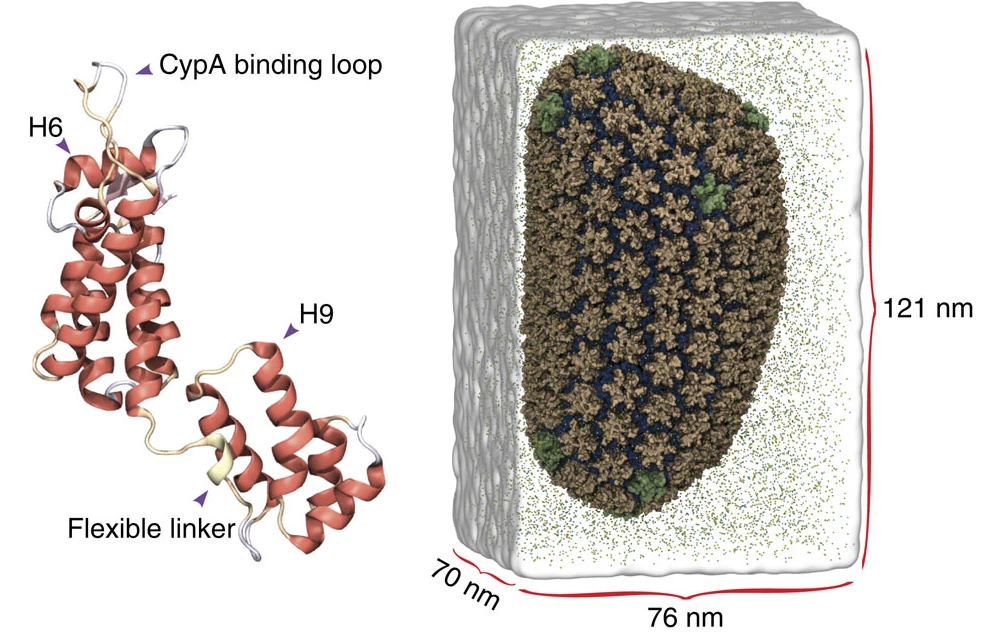
\includegraphics[width=0.9\columnwidth, trim={0cm 0 0cm 0cm}]{figures/Intro/HIV-1.png}
        \caption{MD simulation with 64,423,983 atoms of the HIV-1 capsid. Perilla et al.~\cite{Perilla2017} investigated properties of the HIV-1 capsid at an atomic resolution.}
        \label{fig:hiv_capsid}
    \end{figure}

    \begin{figure}[H]
        \centering
        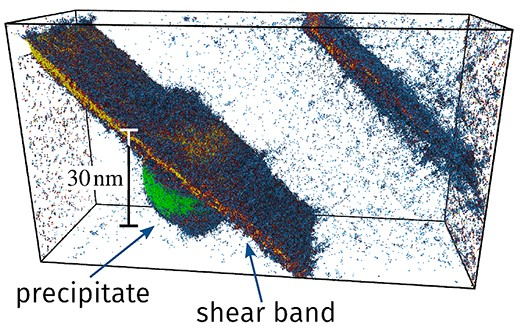
\includegraphics[width=0.9\columnwidth,trim={0cm 0 0cm 0cm}]{figures/Intro/metallic-glass-crack.jpg}
        \caption{MD simulations of shear band formation around a precipitate in metallic glass, as demonstrated by Brink et al.~\cite{Brink2016}.}
        \label{fig:md_simulation_loop}
    \end{figure}
\end{multicols*}

Simulating such systems is very computationally demanding and typically requires the use of high-performance computing (HPC) systems for large-scale simulations. Another challenge is the development of efficient simulation software that can handle the complexity of the systems and make optimal use of the available computational resources. This thesis focuses on the development of AutoPas, a high-performance, auto-tuned particle simulation library for many-body systems, which tries to address these challenges by dynamically switching between algorithms and data structures to guarantee high performance throughout the simulation.

This switching mechanism is guided by so-called \textit{tuning strategies}, which are responsible for exploring the space of available algorithms and data structures and attempt to find appropriate configurations for the current simulation state. The development of efficient tuning strategies is crucial, as efficient choices can significantly reduce the runtime of the simulation, making MD simulations more accessible to researchers and enabling the study of more complex systems.

This thesis focuses on the development of a novel fuzzy logic-based tuning strategy for AutoPas, which allows users to encode their domain knowledge in the tuning process. Furthermore, we investigate a data-driven approach to automatically generate fuzzy systems, and we will show that the proposed fuzzy tuning strategy can outperform existing tuning strategies on specific benchmarks.
\chapter{Theoretical Background}
\label{sec:theoretical_background}


\section{Molecular Dynamics}

% simulation loop


\section{AutoPas}

AutoPas is an open-source library designed to achive optimal performance at the node level for short-range particle simulations. On a high level, AutoPas can be seen as a black-box performing arbitrary N-body simulations with short-range particle interactions. The main goal of AutoPas is to provide a high-level interface for the user to perform simulations without having to worry about the low-level details of the simulation. This is achieved by providing a high-level interface for the user to interact with the library, while the library itself takes care of the low-level details of the force calculations

AutoPas provides many different algorithmic implementations for the problem of N-body simulations each with different trade-offs in terms of performance and memory usage. There is no single implementation that is optimal for all simulation scenarios \todo{find reference}, as the optimal implementation depends on the current simulation state.
AutoPas is designed to be adaptive and is capable of periodically switching between different implementations to achieve the best performance for the current simulation state. This is achieved by allowing AutoPas to automatically tune its internal parameters to find the best implementation for the current simulation state.


Since AutoPas just provides a high-level interface to allow for short-range N-body simulations, the user is responsible for specifying the acting forces between the particles and has full control over the simulation loop. Fortunately AutoPas also provides \texttt{\gls{mdflexible}} which is an example implementation of a typical molecular dynamics simulation.

\section{Autotuning in AutoPas}

AutoPas currently provides k \todo{count how many} tunable parameters which can mostly\footnote{There are some exceptions as some choices of parameters are not compatible with each other.} be combined freely with each other. The parameters can be roughly divided into the following categories:

\begin{enumerate}[label=\textbf{\arabic*.}]
      \item \textbf{Container Options:} \\
            The container options are related to the data structure used to store the particles. The most important categories of data structures in this section are:
            \begin{enumerate}
                  \item \textbf{DirectSum} \\
                        DirectSum does not use any additional data structures to store the particles. Instead, it simply holds a list of all particles and performs a brute-force calculation of the forces between all pairs of particles. This results in a complexity of $O(N^2)$ distance checks in each iteration. This method is simple and does not require any additional data structures but has a very poor complexity, making it completly unsuitable for larger simulations. \textit{Generally shouldn't be used except for very small systems or demonstration purposes.~\cite{VICCIONE2008625}}
                  \item \textbf{LinkedCells} \\
                        LinkedCells segments the domain into a regular cell grid and only considers interactions between particles from neighboring cells. This results in the trade-off of that particles further away than the cutoff radius are not considered for the force calculation. In practice this is not a big issue as all short-range forces drop off quickly with distance anyway. Additionally, LinkedCells provides a high cache hit rate as particles inside the same cell can be stored contiguously in memory. Typically, the cell size is chosen to be equal to the cutoff radius $r_c$, meaning that each particle only needs to check the forces with particles inside the $3\times3\times3$ cell grid around it as all other particles are guaranteed to be further away than the cutoff radius. This reduction in possible interactions can result in a complexity of just $O(N)$ distance checks in each iteration. However, there is still room for improvement as constant factors can be quite high. This is especially obvious, as most of the remaining distance checks performed by LinkedCells still do not contribute to the force calculation~\cite{GRATL2019748}. This trend can be explained due to the uneven scaling sphere and cube volumes especially for higher dimensions. For example, in 3D the ratio of the volume of a sphere with radius $r_c$ to the volume of a cube with side length $3r_c$ is given by:

                        \begin{equation}
                              \frac{\text{Interaction Volume}}{\text{Search Volume}} =
                              \frac{V_{sphere}(r_c)}{V_{cube}(3r_c)} = \frac{\frac{4}{3}\pi r_c^3}{(3r_c)^3} = \frac{4}{81}\pi \approx 0.155
                        \end{equation}

                        This means that only about 15.5\% of all particles present in the $3\times3\times3$ cell grid around a particle are actually within the cutoff radius. By choosing smaller cell sizes, this ratio can be increased, reducing the number of unnecessary distance checks, but the performance gain is quickly offset by the increased overhead of managing more cells. \todo{find reference}
                        \textit{However, still generally good for large, homogeneous\footnote{Homogeneous in this context means that the particles are distributed evenly across the domain. If many particles are concentrated in a small area, the behavior of LinkedCells can quickly resemble that of DirectSum.} systems.}

                  \item \textbf{VerletLists} \\
                        VerletLists is another approach to create neighbor lists for the particles. Contrary to LinkedCells, VerletLists does not rely on a regular grid but instead uses a spherical region around each particle to determine its relevant neighbors.
                        The algorithm creates and maintains a list of all particles present in a sphere within radius $r_c \cdot s$ around each particle, where $r_c$ is the cutoff radius and $s>1$ is the skin factor allowing for a buffer zone around the cutoff radius.
                        By chosing a suitable buffer zone, such that no fast moving particle can enter the cutoff radius unnoticed, it is possible to only recalculate the neighbor list every $n$ iterations. This approach can be beneficial for systems with high particle density and frequent interactions, as the neighbor list only needs to be updated every $n$ iterations. This results in a complexity of $O(N)$ distance checks in each iteration.
                        We can repeate the calculation from above to determine the ratio of the interaction volume to the search volume for VerletLists:

                        \begin{equation}
                              \frac{\text{Interaction Volume}}{\text{Search Volume}} =
                              \frac{V_{sphere}(r_c)}{V_{sphere}(r_c \cdot s)} = \frac{\frac{4}{3}\pi r_c^3}{\frac{4}{3}\pi (r_c \cdot s)^3} = \frac{1}{s^3}
                        \end{equation}

                        This time the ratio can be adjusted by changing the skin factor $s$.         Ideally, the skin factor should be chosen such that the ratio is close to 1. This however reduces the buffer zone around the cutoff radius which means that the neighbor list needs to be updated more frequently. We conclude that choosing a skin factor that is too small can result in particles entering the cutoff radius unnoticed, which can lead to incorrect results, while choosing a skin factor that is too large can result in unnecessary distance checks.

                        Compared to LinkedCells, VerletLists can be constructed such that there are very few unnecessary distance checks. However, the construction of the neighbor list is quite memory intensive and can result in a high memory overhead. Additionally, the neighbor list needs to be updated every $n$ iterations, which can result in a performance overhead.

                        \textit{\todo{when to use VerletLists}}

                        There are again several different implementations of VerletLists in AutoPas, each with different trade-offs in terms of performance and memory usage.

            \end{enumerate}

      \item \textbf{Traversal Options:} \\
            These options are related to the traversal algorithm used to calculate the forces between the particles given a specific container. There are many different traversal algorithms available in AutoPas, each with different trade-offs in terms of performance and optimization potential. In the following we will discuss the most interesting traversal categories:

            \begin{enumerate}

                  \item \textbf{LinkedCells Colored Traversal} \\
                        Since LinkedCells only considers interactions with particles from neighboring cells, it is possible to parallelize the force calculation by calculating forces for particles in different cells in parallel, as long as the particles don't share common neighbors. This parallelization strategy gives rise to many different traversal algorithms, each with different trade-offs in terms of performance and optimization potential. Some important traversal algorithms for LinkedCells are:

                        \todo{add}

                  \item \textbf{VerletLists Traversal} \\
                        Most of the traversal algorithms for VerletLists are based on the same principle of the respective LinkedCells traversal algorithms. The main difference is that the neighbor list is used to determine the particles that need to be considered for the force calculation. Some important traversal algorithms for VerletLists are:


                        \todo{add}
            \end{enumerate}




      \item \textbf{Data Layout Options:} \\
            The Data Layout Options are related to the way the particles are stored in memory. The two possible data layouts are:
            \begin{enumerate}
                  \item \textbf{SoA} \\
                        The SoA (Structure of Arrays) data layout stores the properties of all the particles separate arrays. For example, the x- ,y- and z-coordinates of all particles are stored in separate arrays. This data layout is beneficial for vectorization as the properties of the particles are stored contiguously in memory. This allows for efficient vectorization of the force calculations as the properties of the particles can be loaded into vector registers in a single instruction. \todo{find reference}

                  \item \textbf{AoS} \\
                        The AoS (Array of Structures) data layout stores all particle properties in a big array consisting of structures. This allows for efficient cache utilization as the properties of the same particle are close to each other in memory. However, this data layout is not beneficial for vectorization as the properties of the particles are not stored contiguously in memory. This means that the properties of the particles need to be loaded into vector registers one by one, which can result in inefficient vectorization of the force calculations. \todo{find reference}
            \end{enumerate}



      \item \textbf{Newton 3 Options:} \\
            The Newton 3 Options are related to the way the forces between the particles are calculated. The Newton 3 law states that for every action there is an equal and opposite reaction \todo{cite}. This means that the force between two particles is the same, regardless of which particle is considered the source and which particle is considered the target. In Molecular Dynamics simulations, this rule can be exploited to reduce the number of distance checks needed to calculate the forces between all pairs of particles by a factor of 2. The two possible Newton 3 options are:
            \begin{enumerate}
                  \item \textbf{Newton3 Off} \\
                        If Newton 3 is turned off, the forces between all pairs of particles are calculated twice, once for each particle. This results in a constant overhead of factor 2.

                  \item \textbf{Newton3 On} \\
                        If Newton 3 is turned on, the forces between all pairs of particles are calculated only once. There is no more overhead due to recalculating the forces twice, but turing on Newton 3 requires additional bookkeeping especially in multi-threaded environments, as there can occur race conditions when updating the forces of the particles. \todo{find reference}
                        \textit{Generally should be turned on, \todo{find reference}}
            \end{enumerate}

\end{enumerate}

\section{Fuzzy Logic}

\section{Fuzzy Tuning}



\chapter{Implementation}
\label{sec:implementation}

\newcommand{\fuzzySetNodeOneD}[4]{
  \begin{tikzpicture}
    \begin{axis}%
      [
        axis line style={black},
        width=4.5cm,
        height=3cm,
        axis lines=center,
        xlabel={#1},
        x label style={at={(axis description cs:0.9,0.25)},anchor=north},
        ylabel=$\mu$,
        y label style={at={(axis description cs:0.5,1)},anchor=south},
        xmin=-6,
        xmax=6,
        ytick={},
        yticklabels={},
        extra x ticks={0},
        extra x tick labels={#3},
        ymax=1,
        samples=25,
        extra y ticks={1},
        every axis plot/.append style={thick}
      ]
      \addplot[red]  {#4};
    \end{axis}
    \node[above,font=\large\bfseries,inner sep=5pt] at (current bounding box.north) {\shortstack{FuzzySet\\#2}};
  \end{tikzpicture}
}

\newcommand{\fuzzySetNodeTwoD}[4]{
  \begin{tikzpicture}
    \begin{axis}%
      [
        width=5.5cm,
        height=4cm,
        axis lines=center,
        xlabel={#1},
        x label style={at={(axis description cs:0.1,0.4)},anchor=north},
        ylabel={#2},
        y label style={at={(axis description cs:0.4,-0.15)},anchor=south},
        zlabel=$\mu$,
        z label style={at={(axis description cs:0.5,0.95)},anchor=south},
        xmin=-6,
        xmax=6,
        colormap/viridis,
        view={10}{40},
        ymin=-6,
        ymax=6,
        zmin=0,
        zmax=1,
      ]
      \addplot3 [
        domain=-6:6,
        samples = 20,
        surf,
      ]{#4};
    \end{axis}
    \node[above,font=\large\bfseries,inner sep=5pt] at (current bounding box.north) { \shortstack{FuzzySet\\#3}};
  \end{tikzpicture}
}


This chapter describes the implementation of the Fuzzy Tuning technique in AutoPas. The implementation is divided into three main parts: the generic fuzzy logic framework, the rule parser, and the fuzzy tuning Strategy. The fuzzy logic framework is the core of this implementation and implements the mathematical foundation of this technique. The rule parser loads the supplied knowledge base from a rule file. Finally, the Fuzzy Tuning Strategy implements the interface between the fuzzy logic framework and the AutoPas simulation. It is responsible for updating the configuration queue to select configurations to be tested next.


\section{Fuzzy Tuning Framework}

The Fuzzy Tuning framework implements the mathematical foundation of the Fuzzy Tuning technique. It consists of several components that fully implement the mathematical concepts of fuzzy logic. It consists of the following components:

\begin{itemize}
  \item \textbf{Crisp Set}\\
        The Crisp Set class models classical sets using k-cells\footnote{A k-cell is a hyperrectangle in the k-dimensional space constructed from the Cartesian product of k intervals $C = I_1 \times I_2 \times \ldots \times I_k$ where $I_i = [x_{low}, x_{high}] \subset \mathbb{R} $ is an interval in the real numbers.} in order to represent the universe of discourse for the fuzzy sets. Therefore, it keeps track of the ranges of the input variables, which are later used in the defuzzification step.
        Using k-cells, we can only model continuous variables with a finite range of values. This is an acceptable limitation for the current use case in AutoPas, as all relevant parameters either fulfill this requirement or can be encoded as such (See \autoref{sec:componentTuningApproach}). However, there exist methods to directly use nominal values as described in \cite{ReydelCastillo2012} or \cite{Jodoin2006}, but those are not implemented in this work.\\


  \item \textbf{Fuzzy Set} \\
        As mentioned previously, fuzzy sets consist of a membership function $\mu: X \rightarrow [0, 1]$, assigning a degree of membership to each element of the associated Crisp Set $C$. For the implementation in C++, we distinguish between two types of membership functions: The \texttt{BaseMembershipFunction} and the \texttt{CompositeMembershipFunction}. The \texttt{BaseMembershipFunction} implements membership functions over 1-dimensional k-cells ($1$-cells), typically the real numbers $\mathbb{R}$. It implements the \emph{conventional} type of membership function and is implemented as a lambda function $f: \mathbb{R} \rightarrow [0, 1]$ that directly assigns the degree of membership to each input value. Generic examples of triangular, trapezoidal, gaussian, and sigmoid-shaped membership functions are implemented this way and can be selected by the user via the rule file. \\
        \smallskip
        The \texttt{CompositeMembershipFunction} implements membership functions over  $k$-cells. This distinction is necessary, as we will later use a recursive approach to construct complex fuzzy sets from simpler ones, and those newly constructed fuzzy sets should compose their children's membership functions to calculate their own membership value. Thus requiring a different interface than the \texttt{BaseMembershipFunction}. The \texttt{CompositeMembershipFunctions} are primarily meant to define fuzzy sets resulting from applying logical operations. To demonstrate the concept, let us consider the fuzzy set $\tilde{C} = \tilde{A} \cap \tilde{B}$. This new fuzzy set $\tilde{C}$ is defined over the Crisp Set $C = A \times B$, where $A$ and $B$ are the Crisp Sets of the fuzzy sets $\tilde{A}$ and $\tilde{B}$, respectively. As explained in previous chapters, the membership function $\mu_{\tilde{C} : C \rightarrow [0, 1]}$ can be calculated as $\mu_{\tilde{C}}(x, y) = \min(\mu_{\tilde{A}}(x), \mu_{\tilde{B}}(y))$, by recursively making use of the membership functions of the \emph{child} fuzzy sets $\tilde{A}$ and $\tilde{B}$. The only new information the \texttt{CompositeMembershipFunction} needs to store is the function that should be used to combine the membership values of the children. As these membership functions operate in a higher-dimensional space, they are implemented as lambda functions $f: \mathbb{R}^k \rightarrow [0, 1]$ combining the membership values of their \emph{children} using some logical operation to produce their own membership values. The logical operations $\min$, $\max$, and $\neg$ are implemented this way as they combine existing fuzzy sets to form new ones. \\
        \smallskip
        Internally, all fuzzy sets are represented using a tree-like data structure. The tree's root node represents the fuzzy set itself, and every internal node represents an intermediate fuzzy set defining the smaller fuzzy sets, which can be combined to form the root fuzzy set. In this tree structure, the \texttt{CompositeMembershipFunctions} act as a link between existing fuzzy sets (the \emph{children}) and lead to the definition of a more complex fuzzy set (the \emph{parent}). The Leaf nodes of a fuzzy set can no longer be decomposed into simpler fuzzy sets and are consequently defined using the \texttt{BaseMembershipFunctions}.
        \autoref{fig:modularfuzzysetconstruction} shows a larger example of how complex fuzzy sets can be constructed from simpler fuzzy sets using the \texttt{CompositeMembershipFunctions} and \texttt{BaseMembershipFunctions}. \\
        Furthermore, the Fuzzy Set class provides methods for defuzzification and combining fuzzy sets using logical operations.

  \item \textbf{Linguistic Variable}\\
        Linguistic variables act as simple containers for fuzzy sets. Each Linguistic Variable has a name (e.g., \texttt{Temperature}) and stores linguistic terms consisting of a name (e.g., \texttt{hot}) and a corresponding fuzzy set $\tilde{H}$ describing the distribution of the term.

  \item \textbf{Fuzzy Rule}\\
        The Fuzzy Rule class stores an antecedent and a consequent fuzzy set ($\tilde{A}$ and $\tilde{C}$). Additionally, the class provides a method to apply the rule, producing a new fuzzy set $R=\tilde{C}\uparrow \mu$ consisting of the partially activated fuzzy set $\tilde{C}$ where $\mu$ is the degree of membership of the supplied input values in the antecedent fuzzy set $\tilde{A}$.

  \item \textbf{Fuzzy System:} The Fuzzy System combines all the concepts described above to create a system that can evaluate a set of fuzzy rules and generate a defuzzified output value based on the supplied input values. Such a system acts like a black box $f: \mathbb{R}^n \rightarrow \mathbb{R}$ that maps crisp input values to a crisp output value. Multiple such systems are used in later sections to implement the tuning strategy.
\end{itemize}

A simplified class diagram of the implementation can be seen in \autoref{fig:classdiagram}.

\newpage

\begin{figure}[H]
  \centering
  \includesvg[width=\textwidth]{figures/class-diagram.svg}
  \caption[Class diagram of the Fuzzy Tuning Strategy]{Simplified class diagram of the Fuzzy Tuning strategy. There is a clear separation between implementing the Fuzzy Logic framework and the tuning strategy. This allows for an easy reuse of the Fuzzy Logic framework in other parts of AutoPas if desired.}
  \label{fig:classdiagram}
\end{figure}


\newpage




\begin{figure}[H]
  \centering
  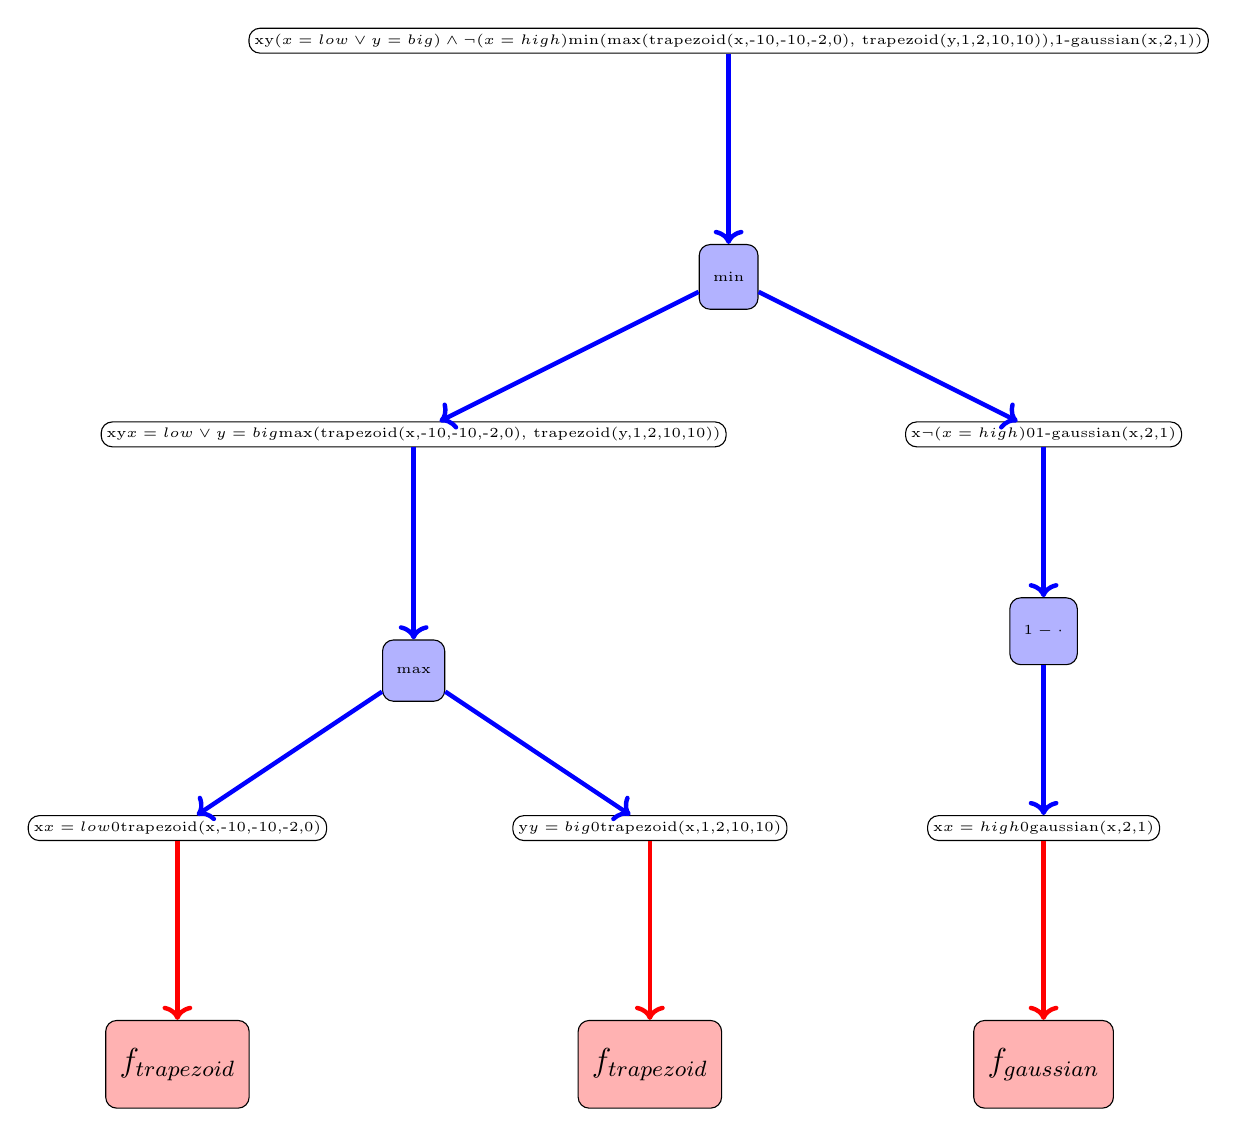
\begin{tikzpicture}[scale=2,font=\tiny]


    \node [rectangle, rounded corners, draw, inner sep=2pt] (A) at (0,0) {
      \fuzzySetNodeTwoD{x}{y}{$(x=low \lor y=big) \land \neg (x = high)$}{min(max(trapezoid(x,-10,-10,-2,0), trapezoid(y,1,2,10,10)),1-gaussian(x,2,1))}
    };

    \node [rectangle,rounded corners,draw,inner sep=5pt, inner ysep=10pt,fill=blue!30] (X) at (0,-1.5) {
      $\min$
    };


    \node [rectangle,rounded corners,draw,inner sep=2pt] (B) at (-2,-2.5) {
      \fuzzySetNodeTwoD{x}{y}{$x=low \lor y=big$}{max(trapezoid(x,-10,-10,-2,0), trapezoid(y,1,2,10,10))}
    };

    \node [rectangle,rounded corners,draw,inner sep=2pt] (C) at (2,-2.5) {
      \fuzzySetNodeOneD{x}{$\neg (x = high)$}{0}{1-gaussian(x,2,1)}
    };


    \node [rectangle,rounded corners,draw,inner sep=5pt, inner ysep=10pt,fill=blue!30] (Y) at (-2,-4) {
      $\max$
    };

    \node [rectangle,rounded corners,draw,inner sep=5pt, inner ysep=10pt,fill=blue!30] (Z) at (2,-3.75) {
      $1 - \cdot$
    };


    \node [rectangle,rounded corners,draw,inner sep=2pt] (D) at (-3.5,-5) {
      \fuzzySetNodeOneD{x}{$x = low$}{0}{trapezoid(x,-10,-10,-2,0)}
    };

    \node [rectangle,rounded corners,draw,inner sep=2pt] (E) at (-0.5,-5) {
      \fuzzySetNodeOneD{y}{$y = big$}{0}{trapezoid(x,1,2,10,10)}
    };

    \node [rectangle,rounded corners,draw,inner sep=2pt] (F) at (2,-5) {
      \fuzzySetNodeOneD{x}{$x = high$}{0}{gaussian(x,2,1)}
    };



    \node [rectangle,rounded corners,draw,inner sep=5pt, inner ysep=10pt,fill=red!30] (G) at (-3.5,-6.5) {
      \large $f_{trapezoid}$
    };

    \node [rectangle,rounded corners,draw,inner sep=5pt, inner ysep=10pt,fill=red!30] (H) at (-0.5,-6.5) {
      \large $f_{trapezoid}$
    };

    \node [rectangle,rounded corners,draw,inner sep=5pt, inner ysep=10pt,fill=red!30] (I) at (2,-6.5) {
      \large $f_{gaussian}$
    };


    \draw[->,ultra thick,draw = blue] (A) -- (X);
    \draw[->,ultra thick,draw = blue] (X) -- (B);
    \draw[->,ultra thick,draw = blue] (X) -- (C);


    \draw[->,ultra thick,draw = blue] (B) -- (Y);
    \draw[->,ultra thick,draw = blue] (Y) -- (D);
    \draw[->,ultra thick,draw = blue] (Y) -- (E);

    \draw[->,ultra thick,draw = blue] (C) -- (Z);
    \draw[->,ultra thick,draw = blue] (Z) -- (F);

    \draw[->,ultra thick,draw = red] (D) -- (G);
    \draw[->,ultra thick,draw = red] (E) -- (H);
    \draw[->,ultra thick,draw = red] (F) -- (I);
  \end{tikzpicture}

  \caption[Recursive construction of a complex fuzzy set from simpler fuzzy sets.]{Recursive construction of a complex fuzzy set from simpler fuzzy sets. Using the linguistic variables $x$ with the terms $\{low, high\}$ and $y$ with the terms $\{big, small\}$ we can construct the fuzzy set $(x=low \lor y=big) \land \neg (x = high)$ by combining the fuzzy sets $x=low \lor y=big$ and $\neg (x = high)$. Those fuzzy sets are again constructed from the simpler fuzzy sets $x=low$, $y=big$ and $x=high$.

    The fuzzy sets at the leaf level can be directly constructed using predefined \textcolor{red}{\texttt{BaseMembershipFunctions}} (e.g., trapezoid, sigmoid, gaussian \dots) and provide the foundation for the more complex fuzzy sets
    All other fuzzy sets are created by combining other fuzzy sets using \textcolor{blue}{\texttt{CompositeMembershipFunctions}}. The logical operators $\min$, $\max$, and $1 - \cdot$ are implemented this way, as they directly act on top of other fuzzy sets.}
  \label{fig:modularfuzzysetconstruction}
\end{figure}


\section{Rule Parser}

The Rule Parser is responsible for parsing the knowledge base supplied by the user and converting it into the internal representation used by the Fuzzy Tuning framework. It is based on the ANTLR4\footnote{https://www.antlr.org/} parser generator and makes use of a domain-specific language tailored to the needs of the Fuzzy Tuning. The language is designed to be lightweight and directly incorporates aspects of AutoPas, such as configurations, into the rule file. All supplied rules predicting values for the same output variable are grouped together, forming a single Fuzzy System. \\
The conversion between the generated parse tree and the internal representation is done by a visitor pattern that traverses the parse tree generated by ANTLR4 and internally builds the corresponding object hierarchy.
A minimal example demonstrating the syntax of the rule file can be seen in \autoref{lst:rulefile}.

\begin{lstlisting}[caption={Demonstration of the domain-specific language used for Fuzzy Tuning},label={lst:rulefile},language=FuzzyLanguage]
# Define the settings of the fuzzy systems
FuzzySystemSettings:
    defuzzificationMethod:  "meanOfMaximum"
    interpretOutputAs:      "IndividualSystems"

# Define linguistic variables and their linguistic terms
FuzzyVariable: domain: "homogeneity" range: (-0.009, 0.1486)
    "lower than 0.041":     SigmoidFinite(0.0834, 0.041, -0.001)
    "higher than 0.041":    SigmoidFinite(-0.001, 0.041, 0.0834)

FuzzyVariable: domain: "threadCount" range: (-19.938, 48.938)
    "lower than 18.0":      SigmoidFinite(38.938, 18.0,  -2.938)
    "lower than 26.0":      SigmoidFinite(46.938, 26.0,   5.061)
    "lower than 8.0":       SigmoidFinite(28.938,  8.0, -12.938)
    "higher than 18.0":     SigmoidFinite(-2.938, 18.0,  38.938)
    "higher than 26.0":     SigmoidFinite(5.0617, 26.0,  46.938)
    "higher than 8.0":      SigmoidFinite(-12.93,  8.0,  28.938)
     
FuzzyVariable: domain: "particlesPerCellStdDev" range: (-0.017, 0.072)
    "lower than 0.013":     SigmoidFinite(0.0639, 0.038,  0.012)
    "higher than 0.013":    SigmoidFinite(0.012,  0.013,  0.0639)
  
FuzzyVariable: domain: "Newton 3" range: (0, 1)
    "disabled, enabled":   Gaussian(0.3333, 0.1667)
    "enabled":             Gaussian(0.6667, 0.1667)
      
# Define the interpretation of the output variables in the context of AutoPas
OutputMapping:
 "Newton 3":
     0.333 => [newton3 = "disabled"], [newton3 = "enabled"]
     0.666 => [newton3 = "enabled"]

# Define rules connecting the input variables to the output variables
if ("threadCount" == "lower than 18.0") && ("threadCount" == "higher than 8.0") 
     && ("homogeneity" == "lower than 0.041")
   then ("Newton 3" == "enabled")
if ("threadCount" == "higher than 26.0") && ("particlesPerCellStdDev" == "lower than 0.013")
   then ("Newton 3" == "disabled, enabled")
\end{lstlisting}



\section{Tuning Strategy}

The Tuning Strategy implements the interface between the Fuzzy Tuning framework and the AutoPas simulation and is responsible for updating the configuration queue of configurations to be tested next. To achieve this, the strategy evaluates all fuzzy systems present in the rule file using the \emph{LiveInfoData} (See \ref{des:liveinfodatafields}) collected by AutoPas. These data points contain summary statistics about various aspects of the current simulation state, such as the total number of particles, the average particle density, or the average homogeneity of the particle distribution. Each evaluation of a Fuzzy System yields a single numeric value, which is then passed on to the \texttt{OutputMapper} object. The \texttt{OutputMapper} is responsible for mapping the continuous output value of the Fuzzy System to the discrete configuration space of AutoPas.

Internally, the \texttt{OutputMapper} stores an ideal numerical location for each configuration-pattern\footnote{A configuration-pattern is a tuple of all tunable parameters, where each component of the tuple describes a set of possible values for this parameter. The wildcard value \texttt{*} allows any possible value. For example, the configuration-pattern \texttt{(Container=LinkedCells, Traversal=*, DataLayout=SoA, Newton3=enabled)} matches the specified configuration, regardless of the value of the \texttt{Traversal} parameter.} and always selects the option closest to the predicted value. This method of assigning discrete values to the output of fuzzy systems is inspired by Mohammed et al.~\cite{Mohammed2022}'s work on scheduling algorithms, where the authors used a similar approach.

All the configuration patterns predicted by the Fuzzy Systems are then collected and used to update AutoPas's configuration queue. In the following iterations, AutoPas will benchmark every selected configuration for a few iterations and evaluate its performance based on the chosen metric. The best configuration is then declared the winner of this tuning phase and is used for the following simulation phase.

Currently, two different approaches using Fuzzy Tuning to predict \emph{optimal} configurations are implemented: The \emph{Component Tuning Approach} and the \emph{Suitability Tuning Approach}. Both approaches are described in detail in the following sections.


\subsection{Component Tuning Approach}
\label{sec:componentTuningApproach}

The Component Tuning Approach assumes that each tunable parameter can be tuned independently of the others, making it possible to define a separate Fuzzy System for each tunable parameter.

All those Fuzzy Systems should then attempt to predict the best value of their parameter independent of the other parameters. This approach requires the rule file to only define $\#Parameters$ different Fuzzy Systems and a corresponding \texttt{OutputMapper} for each parameter. Creating such rule files is straightforward and could be reasonably created manually by a domain expert. An obvious drawback of this method is the independence assumption between the parameters, which might not hold in practice. However, the practical Experiments carried out in \autoref{sec:comparison_and_evaluation} still show quite good results, even with this simplification.

Another problem of this approach lies in the defuzzification step. As this method relies on defining a single system for all values of a tunable parameter, we must define a numerical \emph{ranking} of all those values. Such a ranking is problematic, as most tunable variables are nominal and thus do not have a natural order. To circumvent this problem, we chose the MOM method. It selects the mean of all $x$-values for which the membership function is maximal. When using Gaussian-shaped membership functions for the output values, this method will always return the mean of the Gaussian with the highest activation\footnote{There are exceptions when two Gaussians have the same level of activation, in which case the mean of both Gaussians is returned. However, this rarely happens in practice and could be resolved with other defuzzification methods such as SOM (Smallest of Maxima). The current implementation just uses the MOM method as it works well in practice.}.

The OutputMapper is set up such that the mean values of the Gaussian membership functions are directly mapped to the corresponding values of the tunable parameters. After evaluating this ruleset, one ends up with a list of configuration patterns, each demanding a specific value for their parameter. All those patterns are then used to purge the configuration queue, excluding every configuration that does not match all the predicted patterns. \autoref{fig:fuzzySystemComponent} shows a schematic of the prediction process for the Component Tuning Approach.



\begin{figure}[H]
  \centering

  \newcommand{\xShift}{0.15}
  \newcommand{\yShift}{0.27}
  \newcommand{\scaleShift}{0.1}
  \begin{tikzpicture}[scale=2,font=\small]
    \node[anchor=east] (L) at (-3,-0.6) {$\text{LiveInfo} \in \mathbb{R}^d$};

    \foreach \name [count=\i from 0] in { Newton3, DataLayout, Traversal, Container}
      {
        \pgfmathsetmacro{\scaleFactor}{1 + \i*\scaleShift}

        \node [rectangle,rounded corners,draw,inner sep=2pt,fill=white!80!black,scale=\scaleFactor,anchor=east] (A) at (0-\i * \xShift,0-\i * \yShift) {
          \begin{tikzpicture}[font=\small]
            \begin{axis}%
              [
                title={FCS [\name]},
                width=3.8cm,
                height=2.2cm,
                axis lines=center,
                xmin=0,
                xmax=4,
                xlabel={$\mathbb{R}$},
                x label style={at={(axis description cs:1,0.2)},anchor=west},
                ylabel=$\mu$,
                y label style={at={(axis description cs:0,0.8)},anchor=east},
                xtick={},
                xticklabels= {},
                ytick={},
                yticklabels={},
                ymax=1,
                every axis plot/.append style={thick},
                domain=0:4
              ]
              \addplot[blue, samples=17] {gaussian(x,1,0.2)};
              \addplot[red,samples=15] {gaussian(x,2,0.2)};
              \addplot[green,samples=17] {gaussian(x,3,0.2)};
            \end{axis}
          \end{tikzpicture}
        };

        \node [rectangle,rounded corners,draw,inner sep=2pt,fill=white!80!black,scale=\scaleFactor*1.1,anchor=east] (O) at (1.45-\i *\xShift*0.2,0-\i*\yShift) {\tiny{OutputMapper}};

        \node[scale=\scaleFactor*1.2, anchor=west] (T) at (1.85-\i*\xShift*0.3,0-\i*\yShift) {\tiny{\name Option}};

        \draw[->, thick] (L.east) -- (A.west) ;

        \draw[->, thick] (A.east) -- (O.west) ;
        \draw[->, thick] (O.east) -- (T.west) ;
      }

  \end{tikzpicture}

  \caption[Visualization of the fuzzy systems for the Component Tuning Approach]{Example Visualization of the fuzzy systems for the Component Tuning Approach. The parameters \texttt{Container}, \texttt{Traversal}, \texttt{DataLayout}, and \texttt{Newton3} are tuned independently. The OutputMapper maps the defuzzified output values to their respective configuration options.}
  \label{fig:fuzzySystemComponent}

\end{figure}


\subsection{Suitability Tuning Approach}

The Suitability Approach mainly differs from the Component Tuning Approach in that it utilizes $\#Container\_options \cdot \#Traversal\_options \cdot \#DataLayout\_options \cdot \#Newton3\_options$ different Fuzzy Systems, one for each possible combination of those parameters. Each Fuzzy System is responsible for predicting the suitability of its configuration.

The advantage of this approach is that there is no need to rank the output values, and one can utilize the power of Fuzzy Systems to interpolate between different predictions. This method uses the default defuzzification method of COG (Center of Gravity) as the possible suitability predictions have a natural order (higher suitability is better). Furthermore, dependencies and incompatibilities between the parameters can be modeled accurately, as each way of combining the parameters is handled with a separate Fuzzy System. The downside of this method is the enormous complexity of the rule file, which quickly becomes infeasible to maintain by hand. Surprisingly, the cost of evaluating all those Fuzzy Systems is negligible compared to the overhead of other tuning strategies, as later experiments in \autoref{sec:comparison_and_evaluation} will show.


After evaluating all Fuzzy Systems and using a trivial OutputMapping, the method yields a list of \texttt{(Configuration, Suitability)} pairs, which can then be used to update the configuration queue. The current implementation selects the highest possible suitability value and then chooses every configuration performing within a certain threshold of the best configuration. Those configurations are then used to overwrite the configuration queue. \autoref{fig:fuzzySystemSuitability} shows a schematic of the prediction process for the Suitability Tuning Approach.

\begin{figure}[H]
  \centering

  \newcommand{\xShift}{0.03}
  \newcommand{\yShift}{0.13}
  \newcommand{\scaleShift}{0.066}

  \begin{tikzpicture}[scale=2,font=\small]
    \node[anchor=east] (L) at (-3.5,-1.5) {$\text{LiveInfo} \in \mathbb{R}^d$};

    \foreach \name [count=\i from 0] in {15,...,1}
      {
        \pgfmathsetmacro{\scaleFactor}{1 + \i*\scaleShift}
        \pgfmathsetmacro{\opacity}{0 + 1*\i/6}
        \pgfmathsetmacro{\arrowThickness}{0.2 + 1.8*\i/16}


        \node [rectangle,rounded corners,draw,inner sep=2pt,fill=white!80!black, fill opacity=\opacity, draw opacity=\opacity,scale=\scaleFactor,anchor=east] (A) at (0-\i * \xShift,0-\i * \yShift) {
          \begin{tikzpicture}[font=\tiny]
            \begin{axis}%
              [
                title={FCS [Combination\textsubscript {\ifthenelse{\name<10}{\name\space}{\name}}]},
                width=3cm,
                height=2cm,
                axis lines=center,
                xmin=0,
                xmax=4,
                xlabel={$\mathbb{R}$},
                x label style={at={(axis description cs:1,0.2)},anchor=west},
                ylabel=$\mu$,
                y label style={at={(axis description cs:0,0.8)},anchor=east},
                xtick={},
                xticklabels= {},
                ytick={},
                yticklabels={},
                ymax=1,
                every axis plot/.append style={thick},
                domain=0:4
              ]
              \addplot[blue, samples=17] {gaussian(x,1,0.2)};
              \addplot[red,samples=15] {gaussian(x,2,0.2)};
              \addplot[green,samples=17] {gaussian(x,3,0.2)};
            \end{axis}
          \end{tikzpicture}
        };

        \node [rectangle,rounded corners,draw,inner sep=2pt,fill=white!80!black, fill opacity=\opacity, draw opacity=\opacity,scale=\scaleFactor*0.8,anchor=east] (O) at (1+\i *\xShift*1,0-\i*\yShift) {\tiny{OutputMapper}};

        \node[scale=\scaleFactor*0.8,fill opacity=\opacity, draw opacity=\opacity, anchor=west] (T) at (1.3+\i*\xShift*1,0-\i*\yShift) {\tiny{ Configuration {\ifthenelse{\name<10}{\name\space}{\name}}}};

        \node[scale=\scaleFactor*0.8,fill opacity=\opacity, draw opacity=\opacity, anchor=west] (S) at (1.3+\i*\xShift*1,-0.2-\i*\yShift) {};

        \draw[->,thick,fill opacity=\opacity, draw opacity=\opacity,] (L.east) -- (A.west) ;

        \draw[->,thick,fill opacity=\opacity, draw opacity=\opacity,] (A.east) -- (O.west) ;
        \draw[->,thick,fill opacity=\opacity, draw opacity=\opacity,] (O.east) -- (T.west) ;

        \draw[thick, fill opacity=\opacity, draw opacity=\opacity]
        (A.east) edge[bend right, looseness=0.5, ->]
        (S.south west) ;
      }

  \end{tikzpicture}

  \caption[Visualization of the fuzzy systems for the Suitability Tuning Approach]{Example Visualization of the fuzzy systems for the Suitability Tuning Approach. Each fuzzy system is responsible for predicting the suitability of a specific combination of tunable values, resulting in an enormous amount of fuzzy systems. The \texttt{(Configuration, Suitability)} pairs are passed to the Fuzzy Tuning Strategy, which then updates the configuration queue}
  \label{fig:fuzzySystemSuitability}
\end{figure}



\chapter{Proof of Concept}
\label{sec:proof_of_concept}

% -------------------------------------------------------------------------------

% parameers: xlabel, center
\newcommand{\fuzzyTreeNode}[2]{
    \begin{tikzpicture}
        \begin{axis}%
            [
                title = {Fuzzy Split: $#1 \leq #2$},
                width=4.5cm,
                height=3cm,
                axis lines=center,
                xlabel={#1},
                x label style={at={(axis description cs:0.9,-0.1)},anchor=north},
                ylabel=$\mu$,
                y label style={at={(axis description cs:0.5,1)},anchor=south},
                xmin=-5,
                xmax=5,
                xtick={},
                xticklabels= {},
                ytick={},
                yticklabels={},
                extra x ticks={0},
                extra x tick labels={#2},
                ymax=1,
                samples=50,
                extra y ticks={1},
                every axis plot/.append style={thick}
            ]
            \addplot[red]  {sigmoid(x,0,-1)};
            \addplot[blue] {sigmoid(x,0,1)};
            \node[anchor=center, red] at (axis cs:-2.9,0.6) {$\mu_{\text{#1smaller#2}}$};
            \node[anchor=center, blue] at (axis cs:3.1,0.6) {$\mu_{\text{#1greater#2}}$};
        \end{axis}

    \end{tikzpicture}
}

\newcommand{\fuzzyTreeLeaf}[1]{
    \begin{tikzpicture}
        \begin{axis}%
            [
                title = {Class: #1},
                width=3.25cm,
                height=2.25cm,
                axis lines=center,
                xlabel={$\text{class}$},
                x label style={at={(axis description cs:0.6,-0.3)},anchor=west},
                ylabel=$\mu$,
                y label style={at={(axis description cs:0.5,1)},anchor=south},
                xmin=-5,
                xmax=5,
                xtick={},
                xticklabels= {},
                ytick={},
                yticklabels={},
                extra x ticks={0},
                extra x tick labels={#1},
                ymax=1,
                samples=10,
                extra y ticks={1},
                every axis plot/.append style={thick}
            ]
            \addplot[black]  {gaussian(x,0,1)};
        \end{axis}

    \end{tikzpicture}
}

% parameers: xlabel, center
\newcommand{\crispTreeNode}[2]{
    \begin{tikzpicture}
        \begin{axis}%
            [
                title = {Crisp Split: $#1 \leq #2$},
                width=4.5cm,
                height=3cm,
                axis lines=center,
                xlabel={#1},
                x label style={at={(axis description cs:0.9,-0.1)},anchor=north},
                ylabel=$\mu$,
                y label style={at={(axis description cs:0.5,1)},anchor=south},
                xmin=-5,
                xmax=5,
                xtick={},
                xticklabels= {},
                ytick={},
                yticklabels={},
                extra x ticks={0},
                extra x tick labels={#2},
                ymin=-0.1,
                ymax=1.1,
                samples=50,
                extra y ticks={1},
                every axis plot/.append style={thick}
            ]
            \addplot[red,domain=-5:-0.6] {step(x,0,-1)};
            \addplot[blue,domain=0.6:5] {step(x,0,1)};
            \addplot[red,domain=0.6:5] {step(x,0,-1)};
            \addplot[blue,domain=-5:-0.6] {step(x,0,1)};

            \node[draw,draw=black,circle,inner sep=1pt,minimum width=3pt,thick] at (axis cs:0,1) {};
            \node[draw,draw=black,circle,inner sep=1pt,minimum width=3pt,thick] at (axis cs:0,0) {};

            \node[anchor=center, red] at (axis cs:-2.9,0.6) {$#1 \leq #2$};
            \node[anchor=center, blue] at (axis cs:3.1,0.6) {$#1 > #2$};
        \end{axis}

    \end{tikzpicture}
}


% -------------------------------------------------------------------------------

This chapter presents a proof of concept for the fuzzy tuning technique and will develop working instantiations of the approaches introduced in the previous chapter.

\smallskip

\noindent Creating rule bases for fuzzy systems is challenging, as it typically requires a profound prior understanding of the system to create meaningful rules. In practice, such knowledge may be difficult to acquire and formalize, as experts may struggle to express their intuition and experience in the precise, structured form required for a fuzzy rule base. However, data-driven approaches can help semi-automate this process by generating an initial set of rules without prior expert knowledge, which can be refined later.

In this work, we will use a data-driven approach based on decision trees proposed by Crockett et al.~\cite{CROCKETT20062809}. This method first trains decision trees to create an initial set of crisp rules. In the second step, the decision trees are converted into so-called fuzzy decision trees, which can then be used to extract the linguistic variables and fuzzy rules.

\section{Data Driven Rule Extraction}

\subsection{Decision Trees}

Decision trees are prevalent machine learning algorithms used for classification and regression tasks. They work by recursively partitioning the input using axis-parallel splits so that the resulting subsets are as pure as possible. In particular, they try to minimize a given impurity metric, such as the Gini impurity $I_G = \sum_{i=1}^{n} p_i(1-p_i)$ of the subsets~\cite{10.5555/2380985}. Since decision trees directly partition the input space into regions with different classes, they can also be depicted using their decision surface if the dimensionality allows it. The decision surface of a decision tree is a piecewise constant function that assigns the predicted class label to each point in the input space of the decision tree. An example decision tree and its decision surface are shown in \autoref{fig:decisionTreeExample} and \autoref{fig:decisionBoundaryExample}, respectively.

\begin{figure}[H]
    \centering
    \begin{subfigure}[t]{0.48\textwidth}
        \centering
        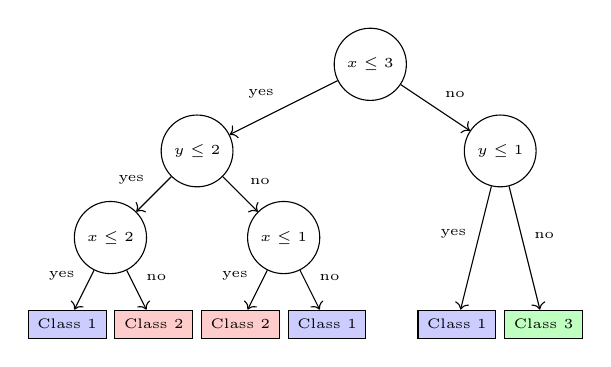
\begin{tikzpicture}[scale=1.1,font=\tiny]
            \node [circle, draw] (A) at (0,0) {$x \leq 3$};
            \node [circle, draw] (B) at (-2,-1) {$y \leq 2$};
            \node [circle, draw] (C) at (1.5,-1) {$y \leq 1$};
            \node [circle, draw] (D) at (-3,-2) {$x \leq 2$};
            \node [circle, draw] (E) at (-1,-2) {$x \leq 1$};

            \node [rectangle,draw,fill=blue!20] (F) at (-3.5,-3) {Class 1};
            \node [rectangle,draw,fill=red!20] (G) at (-2.5,-3) {Class 2};
            \node [rectangle,draw,fill=red!20] (H) at (-1.5,-3) {Class 2};
            \node [rectangle,draw,fill=blue!20] (I) at (-0.5,-3) {Class 1};
            \node [rectangle,draw,fill=blue!20] (J) at (1,-3) {Class 1};
            \node [rectangle,draw,fill=green!25] (K) at (2,-3) {Class 3};

            \draw[->] (A) -- (B) node [midway, left, above left] {yes};
            \draw[->] (A) -- (C) node [midway, right, above right] {no};
            \draw[->] (B) -- (D) node [midway, left, above left] {yes};
            \draw[->] (B) -- (E) node [midway, right, above right] {no};

            \draw[->] (C) -- (J) node [midway, left, above left] {yes};
            \draw[->] (C) -- (K) node [midway, right, above right] {no};

            \draw[->] (D) -- (F) node [midway, left, above left] {yes};
            \draw[->] (D) -- (G) node [midway, right, above right] {no};

            \draw[->] (E) -- (H) node [midway, left, above left] {yes};
            \draw[->] (E) -- (I) node [midway, right, above right] {no};

        \end{tikzpicture}
        \caption[Example decision tree]{Example decision tree}
        \label{fig:decisionTreeExample}
    \end{subfigure}
    \hfill
    \begin{subfigure}[t]{0.48\textwidth}
        \centering
        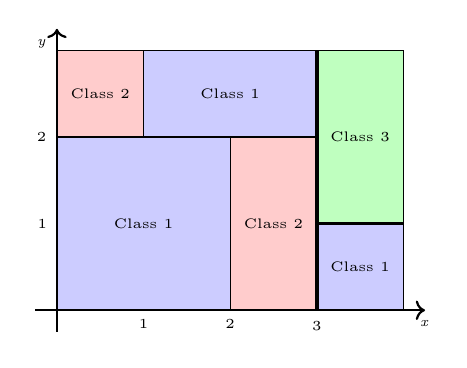
\begin{tikzpicture}[scale=1.1,font=\tiny]

            \draw[fill=red!20] (0,2) -- (1,2) -- (1,3) -- (0,3) -- cycle;

            \draw[fill=blue!20] (1,2) -- (3,2) -- (3,3) -- (1,3) -- cycle;

            \draw[fill=blue!20] (0,0) -- (2,0) -- (2,2) -- (0,2) -- cycle;
            \draw[fill=red!20] (2,0) -- (3,0) -- (3,2) -- (2,2) -- cycle;

            \draw[fill=blue!20] (3,0) -- (4,0) -- (4,1) -- (3,1) -- cycle;
            \draw[fill=green!25] (3,1) -- (4,1) -- (4,3) -- (3,3) -- cycle;

            \draw[->, thick] (-0.25,0) -- (4.25,0) node [below] {\textit{x}};
            \draw[->, thick] (0,-0.25) -- (0,3.25) node [below left] {\textit{y}};

            % decision lines

            \draw[line width=1.5pt,] (3,0) node [below] {3}  -- (3,3) ;
            \draw[line width=1pt] (0,2) node [left] {2} -- (3,2);
            \draw[line width=1pt] (3,1) --  (4,1);

            \draw[] (2,0) node [below] {2}-- (2,2);

            \node [below] at (1,0) {1};

            \node [left] at (0,1) {1};

            % area labels
            \node [] at (0.5,2.5) {Class 2};
            \node [] at (2,2.5) {Class 1};

            \node [] at (1,1) {Class 1};
            \node [] at (2.5,1) {Class 2};


            \node [] at (3.5,2) {Class 3};
            \node [] at (3.5,0.5) {Class 1};

        \end{tikzpicture}
        \caption[Decision surface of the example decision tree]{Decision surface over $\mathcal{D}=[0,4]\times[0,3]$}
        \label{fig:decisionBoundaryExample}
    \end{subfigure}
    \caption{Example decision tree and its decision surface}
\end{figure}



\subsection{Conversion of Decision Trees to Fuzzy Systems}

This section will demonstrate how to convert a classical decision tree into a fuzzy decision system using the fictional decision tree from \autoref{fig:decisionTreeExample} as an example.

\subsubsection{Fuzzy Decision Trees}

Fuzzy decision trees are a generalization of classical decision trees and allow for fuzzy logic to be used in the decision-making process. Instead of following the classical \texttt{if then else} logic to descend into the decision tree, it uses fuzzy sets at each node of the tree to fuzzily calculate the contribution of each branch to the final decision based on the degree of truth of both possible paths. Contrary to classical decision trees, which follow a single path from the root to a leaf node, fuzzy decision trees explore all possible paths simultaneously and make a final decision by aggregating the results of the paths using fuzzy logic operations.

\subsubsection{Conversion}


A classical decision tree is converted into a fuzzy decision tree by replacing the crisp decision (e.g., $x \leq 3$) at each internal node of the decision tree with fuzzy sets. Those fuzzy sets should maintain the same semantics as the crisp decision but should provide a continuous value in the range $[0,1]$ specifying the degree of how much each branch should be considered. Allowing the decision trees to consider multiple paths simultaneously can drastically increase the decision-making capabilities of the decision tree, especially in boundary cases where the decision can be ambiguous.


The shape of the membership functions of the fuzzy sets can be chosen arbitrarily, but typical choices include complementary \texttt{sigmoid}-shaped functions that are centered around the crisp decision boundary (See \autoref{fig:fuzzyMembershipFunctions}), as those function shapes maintain the semantics of the branching idea. Crockett et al.~\cite{CROCKETT20062809} suggested creating those sigmoid shapes with a \emph{width} proportional to the standard deviation of the attribute. In Particular, the authors suggested an interval $[t-n\cdot \sigma, t+n\cdot \sigma]$ for the membership function, where  $t$ is the value of the decision boundary, $\sigma$ is the standard deviation of the attribute and $n$ is a parameter that can be adjusted to control the \emph{width} of the membership function. This interval specifies the region of the membership function where most of the change in membership occurs. The value of $n$ is typically chosen from the interval $n\in [0,5]$ as the membership function can become too broad otherwise and could even weaken the decision-making process~\cite{CROCKETT20062809}. In this work, we will use $n=2$ as a default value.

\begin{figure}[H]
    \centering
    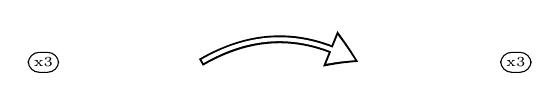
\begin{tikzpicture}[scale=2,font=\tiny]
        \node [rectangle,rounded corners,draw,inner sep=2pt] (A) at (0.5,0) {
            \crispTreeNode{x}{3}
        };

        \node [rectangle,rounded corners,draw,inner sep=2pt] (B) at (3.5,0) {
            \fuzzyTreeNode{x}{3}
        };

        \path[draw=black, line width=1mm, -{Triangle[length=4mm, bend]}]
        (1.5,0) to [bend left] (2.5,0);

        \path[draw=white, line width=0.5mm, -{Triangle[length=3.25mm, bend, angle'=60]}, shorten >= 0.5mm, shorten <= 0.25mm]
        (1.5,0) to [bend left] (2.5,0);

    \end{tikzpicture}
    \caption[Conversion of crisp tree node into fuzzy tree node]{Conversion of crisp membership functions to fuzzy membership functions. The crisp membership functions $x \leq 3$ and $x>3$ of a decision tree node are replaced by two \texttt{sigmoid}-shaped membership functions \textcolor{red}{$\mu_{\text{xsmaller3}}$} and \textcolor{blue}{$\mu_{\text{xgreater3}}$}.}
    \label{fig:fuzzyMembershipFunctions}
\end{figure}

Once the internal nodes of the decision tree have been converted, the next step is to convert the leaf nodes of the decision tree to fuzzy leaf nodes. As the outputs of decision trees are specific class labels, we can define a single linguistic variable consisting of all possible class labels each associated with a fuzzy set. The shapes of the membership functions for the base fuzzy sets can again be chosen mostly arbitrarily, but we will use \texttt{gaussian} functions with a different mean as they are a good choice for representing class labels in a continuous domain.
The resulting conversion of the decision tree in \autoref{fig:decisionTreeExample} into a fuzzy decision tree is shown in \autoref{fig:fuzzyDecisionTreeExample}.


\begin{figure}[H]
    \centering
    \begin{tikzpicture}[scale=1.9,font=\tiny]

        \node [rectangle, rounded corners, draw, inner sep=2pt] (A) at (0,0) {
            \fuzzyTreeNode{x}{3}
        };

        \node [rectangle,rounded corners,draw,inner sep=2pt] (B) at (-2,-1.6) {
            \fuzzyTreeNode{y}{2}
        };

        \node [rectangle,rounded corners,draw,inner sep=2pt] (C) at (1.8,-1.6) {
            \fuzzyTreeNode{y}{1}
        };

        \node [rectangle,rounded corners,draw,inner sep=2pt] (D) at (-3,-3.2) {
            \fuzzyTreeNode{x}{2}
        };

        \node [rectangle,rounded corners,draw,inner sep=2pt] (E) at (-1,-3.2) {
            \fuzzyTreeNode{x}{1}
        };


        \node [rectangle,rounded corners,draw,inner sep=2pt,fill=blue!20] (F) at (-3.7,-4.7) {
            \fuzzyTreeLeaf{1}
        };

        \node [rectangle,rounded corners,draw,inner sep=2pt,fill=red!20] (G) at (-2.6,-4.7) {
            \fuzzyTreeLeaf{2}
        };

        \node [rectangle,rounded corners,draw,inner sep=2pt,fill=red!20] (H) at (-1.5,-4.7) {
            \fuzzyTreeLeaf{2}
        };

        \node [rectangle,rounded corners,draw,inner sep=2pt,fill=blue!20] (I) at (-0.4,-4.7) {
            \fuzzyTreeLeaf{1}
        };

        \node [rectangle,rounded corners,draw,inner sep=2pt,fill=blue!20] (J) at (1.25,-4.7) {
            \fuzzyTreeLeaf{1}
        };

        \node [rectangle,rounded corners,draw,inner sep=2pt,fill=green!20] (K) at (2.35,-4.7) {
            \fuzzyTreeLeaf{3}
        };



        \draw[->] (A) -- (B) node [pos=.4, left, above left] {yes};
        \draw[->] (A) -- (C) node [pos=.4, right, above right] {no};

        \draw[->] (B) -- (D) node [pos=.8, left, above left] {yes};
        \draw[->] (B) -- (E) node [pos=.8, right, above right] {no};

        \draw[->] (C) -- (J) node [pos=.2, left, above left] {yes};
        \draw[->] (C) -- (K) node [pos=.2, right, above right] {no};

        \draw[->] (D) -- (F) node [pos=.6, left, above left] {yes};
        \draw[->] (D) -- (G) node [pos=.6, right, above right] {no};

        \draw[->] (E) -- (H) node [pos=.6, left, above left] {yes};
        \draw[->] (E) -- (I) node [pos=.6, right, above right] {no};
    \end{tikzpicture}

    \caption[Fuzzy decision tree created from the regular decision tree]{The fuzzy decision tree corresponding to the decision tree in \autoref{fig:decisionTreeExample}. Internal nodes use two \texttt{sigmoid} membership functions (\textcolor{red}{$\mu_{\text{smaller}}$} and \textcolor{blue}{$\mu_{\text{greater}}$}) instead of a crisp decision. The leaf nodes use different \texttt{gaussian} membership functions centered around a unique mean.}

    \label{fig:fuzzyDecisionTreeExample}
\end{figure}

It is now possible to fully extract all linguistic variables from the fuzzy decision tree. Every fuzzy set in the tree can be grouped into a corresponding linguistic variable based on the input variable of the fuzzy set. This results in linguistic variables consisting of a bunch of different \texttt{sigmoid} membership functions for input variables (internal nodes) and a single linguistic variable with different \texttt{gaussian} membership functions for the output variable (leaf nodes). The resulting linguistic variables are shown in \autoref{fig:fuzzyDecisionTreeLinguisticVariables}.


\begin{figure}[h]
    \centering

    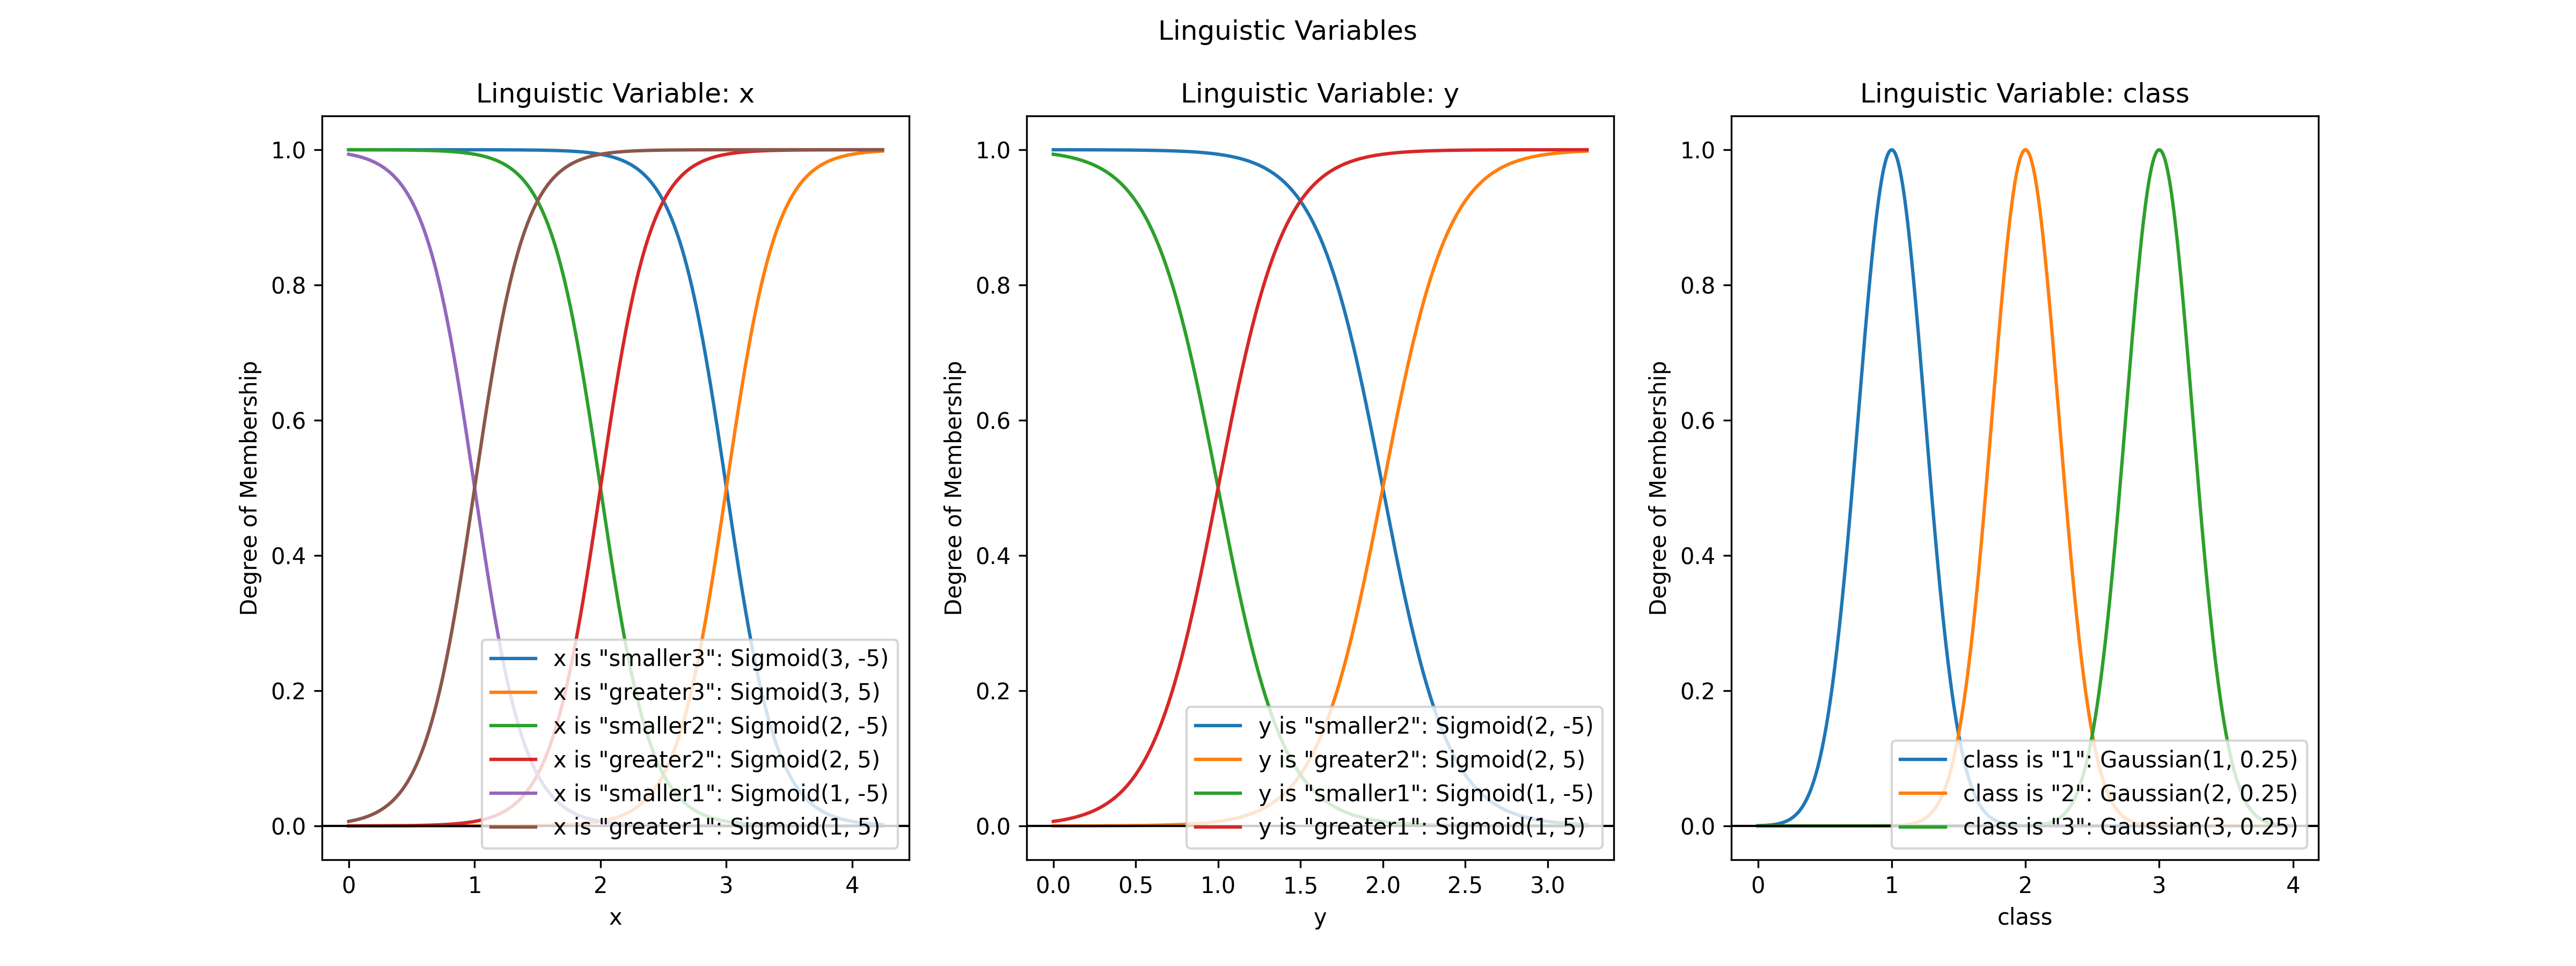
\includegraphics[width=\linewidth]{figures/ProofOfConcepts/fuzzy_sets.png}

    \caption[Linguistic variables for the converted fuzzy decision tree]{Linguistic variables used in the fuzzy decision tree of \autoref{fig:fuzzyDecisionTreeExample}. The standard deviation of the attributes is assumed to be $\sigma \approx 0.5$ such that the \emph{width} of the sigmoid membership functions is $n\cdot \sigma \approx 1$. The standard deviation and placement of the class values are chosen so that they do not overlap too much.}
    \label{fig:fuzzyDecisionTreeLinguisticVariables}
\end{figure}

\subsubsection{Rule Extraction}

The final step is to extract the fuzzy rules from the tree. This can be done by traversing and aggregating the tree in a depth-first manner and collecting the correct membership functions for each path ending in a leaf node along the way. As all conditions of this path have to hold simultaneously, all fuzzy sets are connected using the fuzzy \texttt{AND} operation. This newly created fuzzy set represents the antecedent of the rule. The fuzzy set representing the class (the leaf node) is the consequent of the rule. Therefore, each unique path traversing the tree results in a unique rule of the form \emph{$\text{IF} \; \text{antecedent} \; \text{THEN} \; \text{consequent}$}. This process essentially mimics the decision surface seen in \autoref{fig:decisionBoundaryExample}, as we create precisely one rule for each region of the decision surface. The rules extracted from the fuzzy decision tree in \autoref{fig:fuzzyDecisionTreeExample} using this method are shown in \autoref{tab:fuzzyRulesExample}.


\newcommand{\is}{\textit{ is }}


\begin{table}[H]
    \centering
    \begin{tabular}{c|l|c}
        \textbf{Rule} & \textbf{Antecedent}                                                             & \textbf{Consequent} \\
        \hline
        1             & $x \is \text{smaller3} \land y \is \text{smaller2} \land x \is \text{smaller2}$ & $class \is 1$       \\
        2             & $x \is \text{smaller3} \land y \is \text{smaller2} \land x \is \text{greater2}$ & $class \is 2$       \\
        3             & $x \is \text{smaller3} \land y \is \text{greater2} \land x \is \text{smaller1}$ & $class \is 2$       \\
        4             & $x \is \text{smaller3} \land y \is \text{greater2} \land x \is \text{greater1}$ & $class \is 1$       \\
        5             & $x \is \text{greater3} \land y \is \text{smaller1}$                             & $class \is 1$       \\
        6             & $x \is \text{greater3} \land y \is \text{greater1}$                             & $class \is 3$       \\
    \end{tabular}
    \caption[Extracted fuzzy rules from the example fuzzy decision tree]{Extracted fuzzy rules from the fuzzy decision tree in \autoref{fig:fuzzyDecisionTreeExample} in the format: $\textbf{IF} \text{ Antecedent } \textbf{THEN} \text{ Consequent }$}
    \label{tab:fuzzyRulesExample}
\end{table}

\newpage

\subsubsection{Effect of an Unsuitable Defuzzification Method}

This section briefly discusses the effect of an unsuitable defuzzification method on the resulting fuzzy system. To show the problem when defuzzifying nominal variables, we use the previously extracted rules from \autoref{tab:fuzzyRulesExample} and evaluate the resulting Fuzzy Set for a critical data point $(x=2.95, y=2.5)$ using both the Center of Gravity (COG) and the Mean of Maximum (MOM) defuzzification methods. The resulting fuzzy sets are shown in \autoref{fig:fuzzySetForDataCOG} and \autoref{fig:fuzzySetForDataMOM}.

\begin{figure}[H]
    \centering
    \begin{subfigure}[t]{0.48\textwidth}
        \centering
        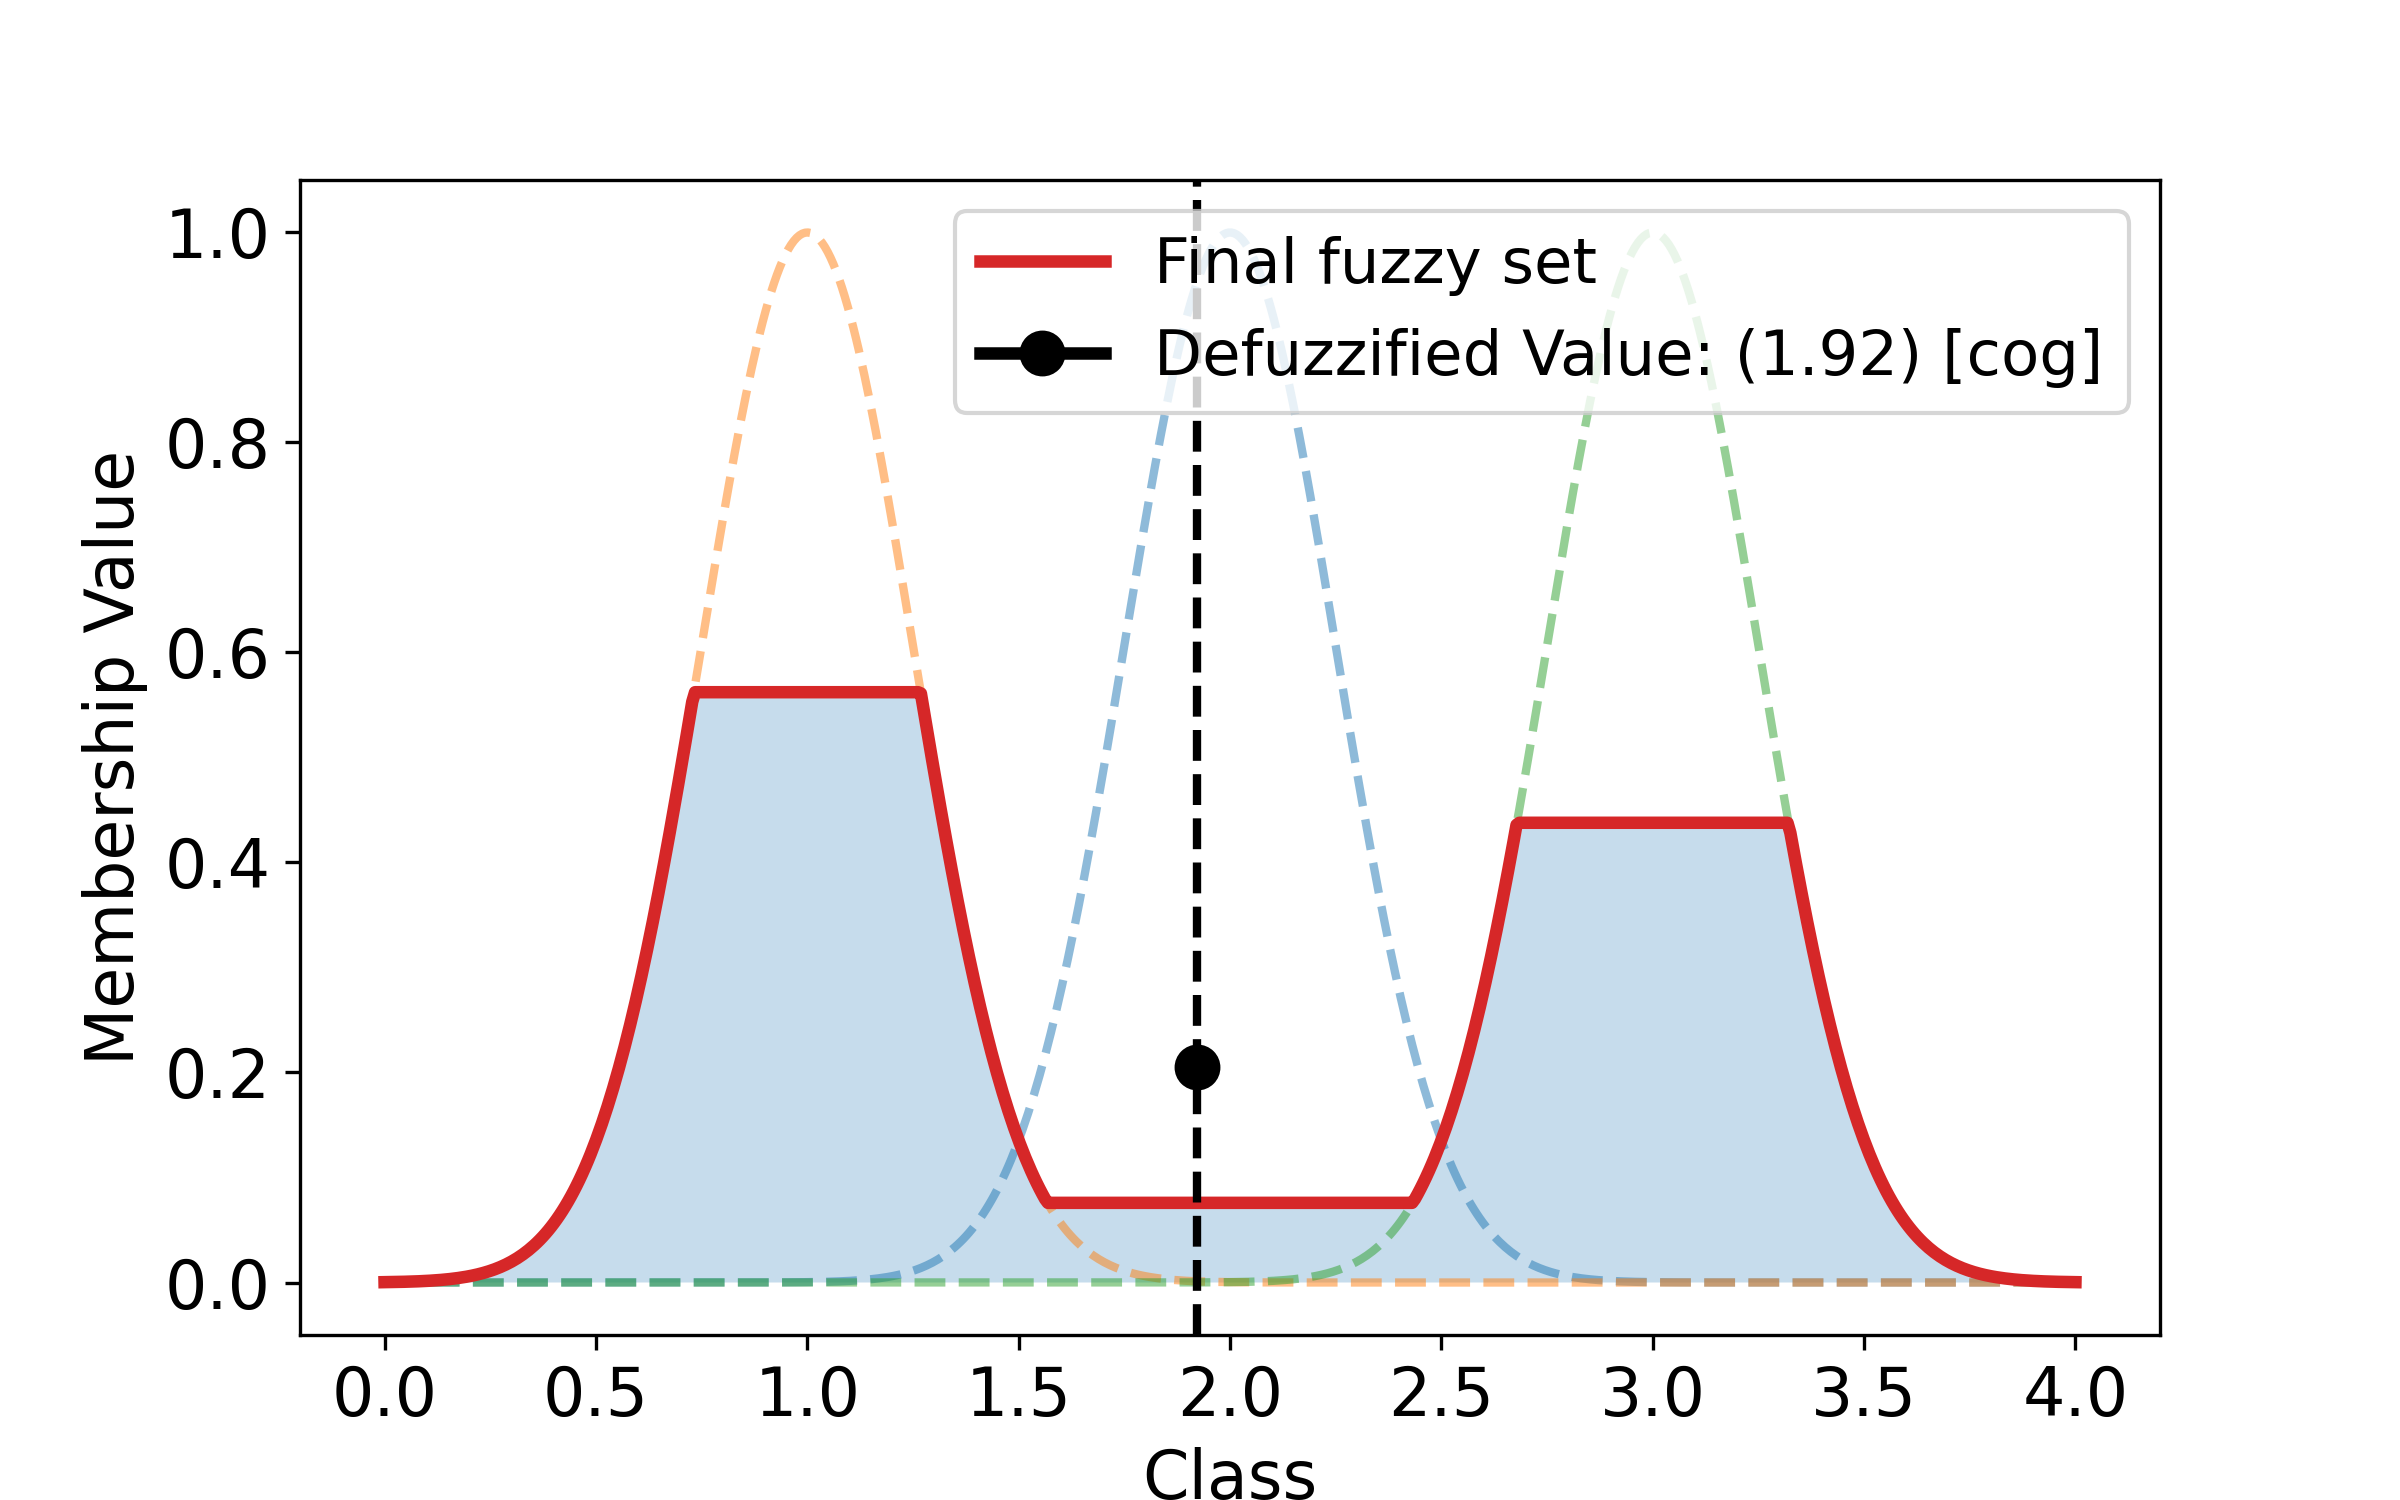
\includegraphics[width=\textwidth,trim={0 0 0 1cm},clip]{figures/ProofOfConcepts/fuzzy_set_for_data_cog.png}
        \caption[Resulting Fuzzy Set after applying the Rules on specific Data, COG Method]{Defuzzification using the COG method. Due to the interpolation, the COG method incorrectly suggests results in a class value close to 2.0 without it being a prominent class.}
        \label{fig:fuzzySetForDataCOG}
    \end{subfigure}
    \hfill
    \begin{subfigure}[t]{0.48\textwidth}
        \centering
        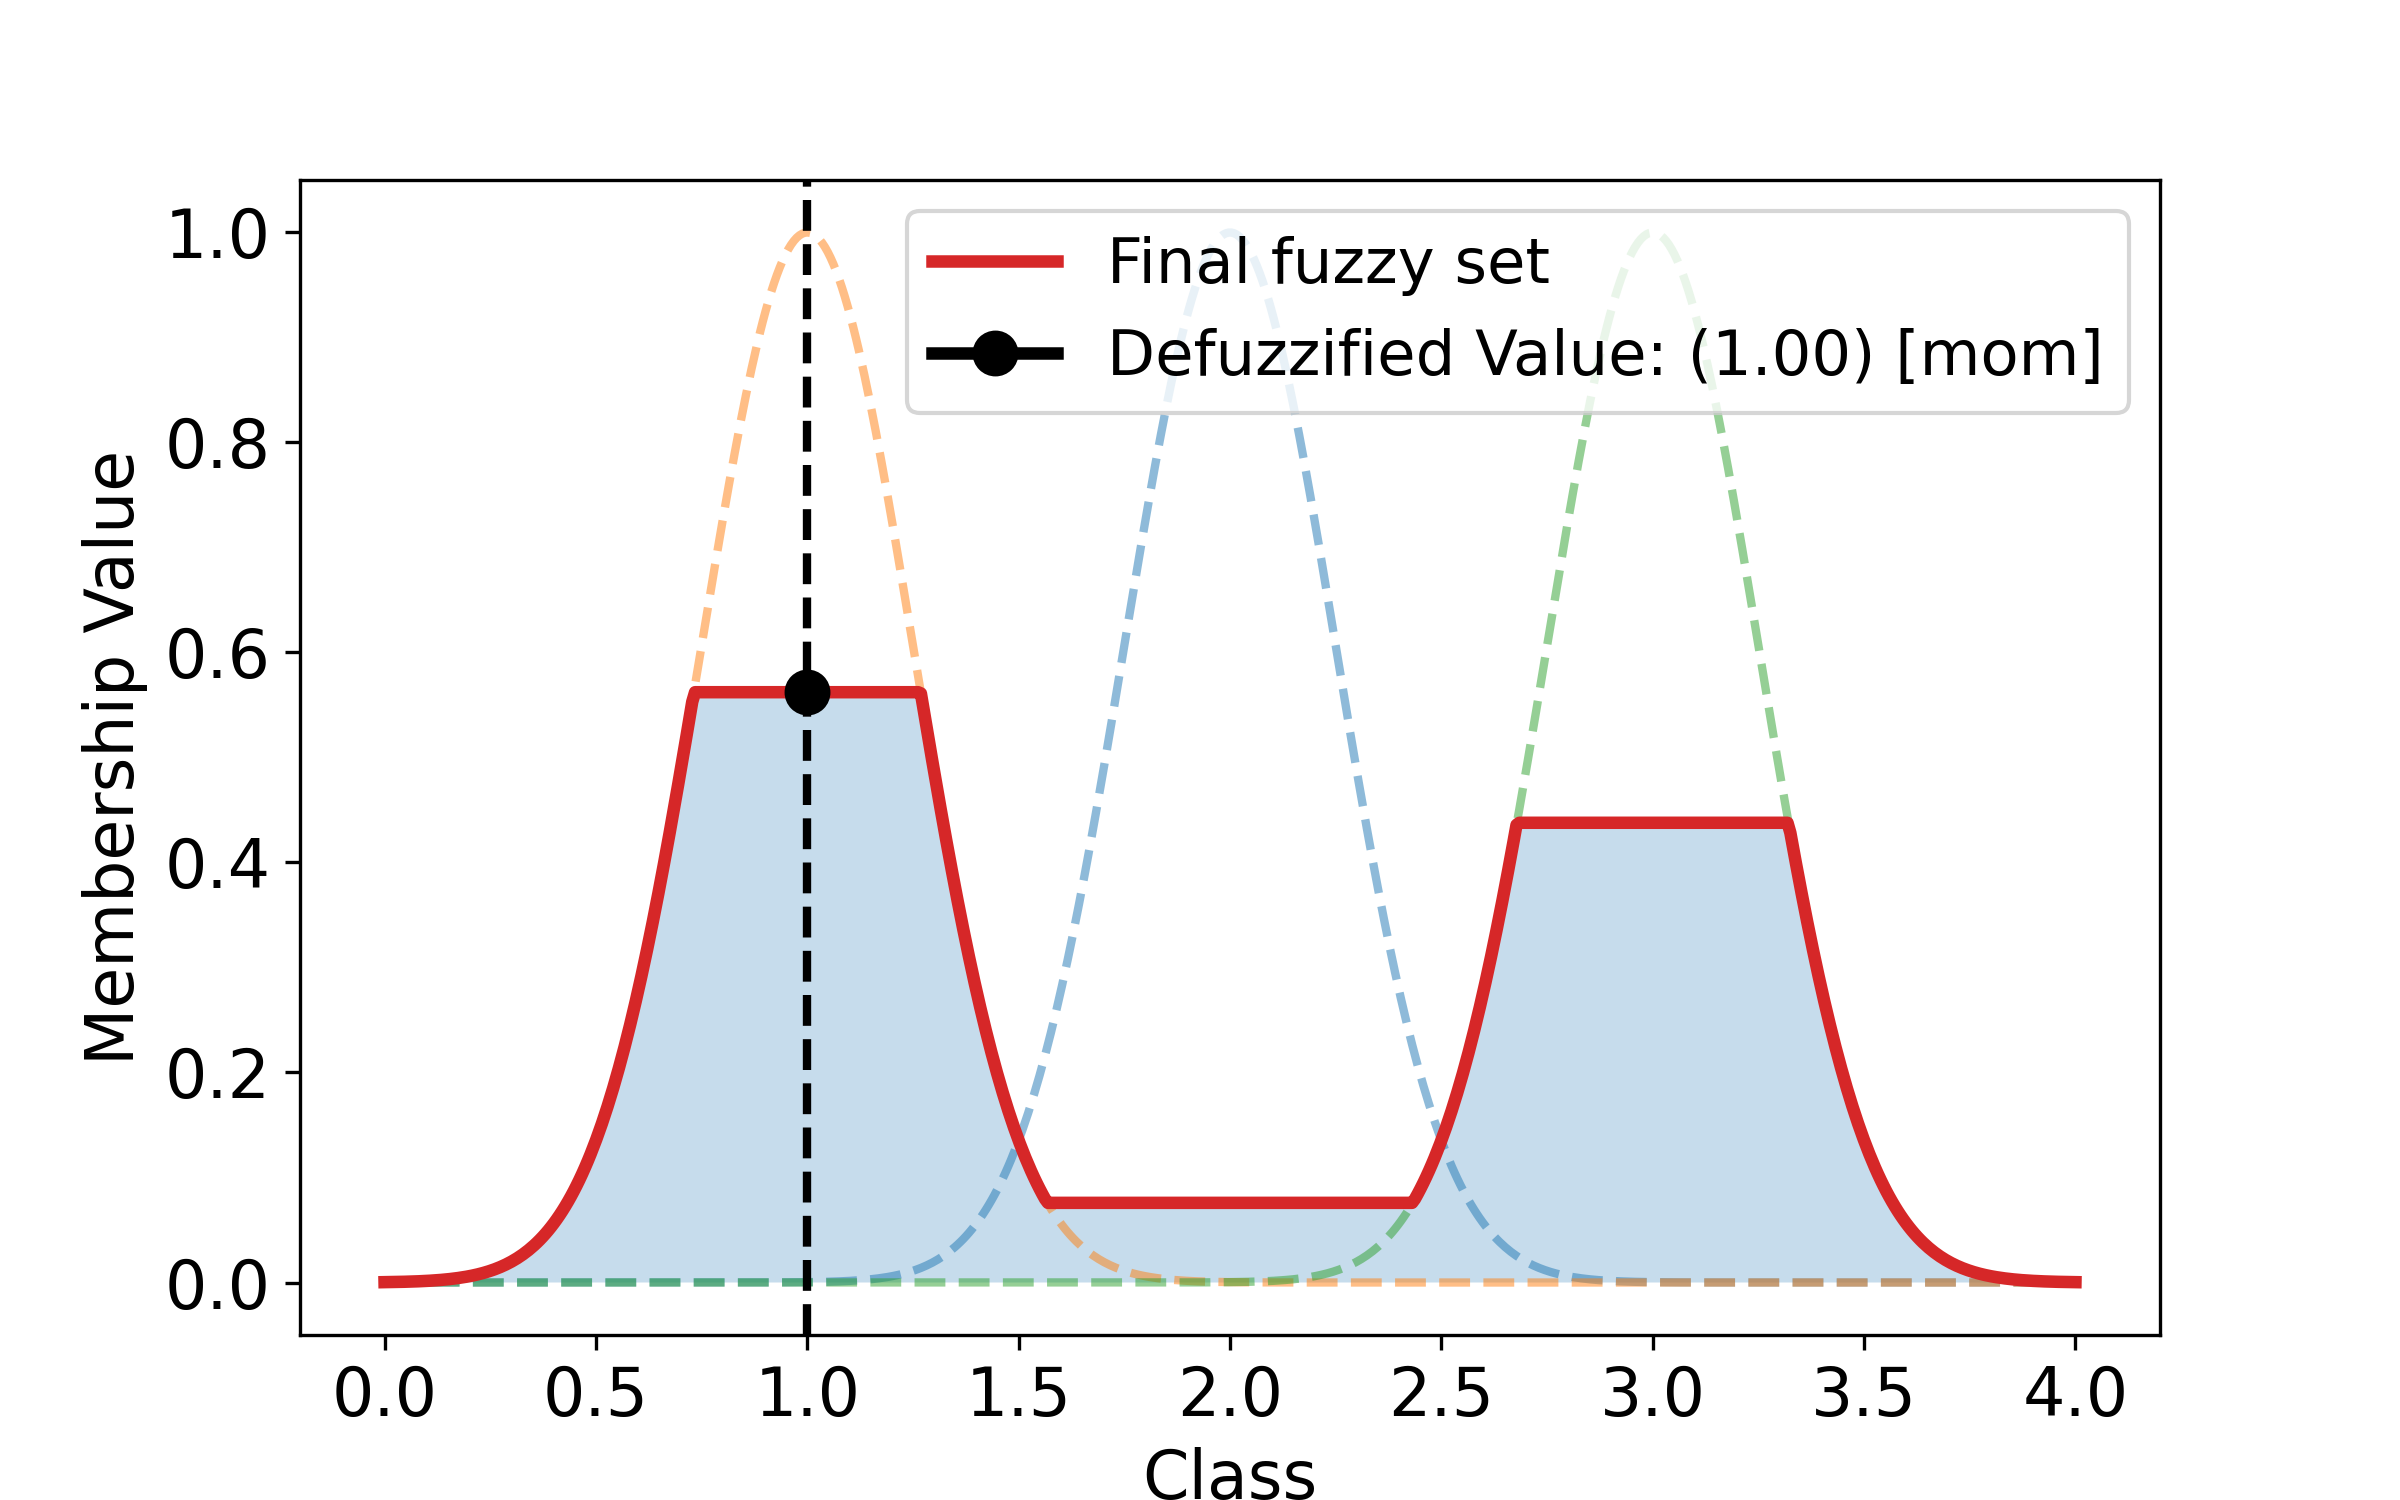
\includegraphics[width=\textwidth,trim={0 0 0 1cm},clip]{figures/ProofOfConcepts/fuzzy_set_for_data_mom.png}
        \caption[Resulting Fuzzy Set after applying the Rules on specific Data, MOM Method]{Defuzzification using the MOM method. The MOM method correctly suggests the class value 1.0 as it is the most prominent class in the fuzzy set.}
        \label{fig:fuzzySetForDataMOM}
    \end{subfigure}
    \caption{Comparison of COG and MOM on data point $(x,y)=(2.95, 2.5)$. }
    \label{fig:fuzzySetComparison}
\end{figure}


To get a full understanding of this problem, we create the full decision surfaces for both fuzzy systems shown in \autoref{fig:fuzzyDecisionSurfaceExampleCOG} and \autoref{fig:fuzzyDecisionSurfaceExampleMOM}, respectively. The decision surface using COG tries to smoothly interpolate between the different classes, which causes interpolation errors if there are other classes in between. The decision surface using MOM is mostly valid and closely resembles the decision surface of the crisp decision tree in \autoref{fig:decisionBoundaryExample}. Consequently, we should use the MOM method when working with nominal variables.

\begin{figure}[H]
    \centering
    \begin{subfigure}[t]{0.45\textwidth}
        \centering
        \begin{tikzpicture}
            \node[anchor=south west,inner sep=0] (image) at (0,0) { 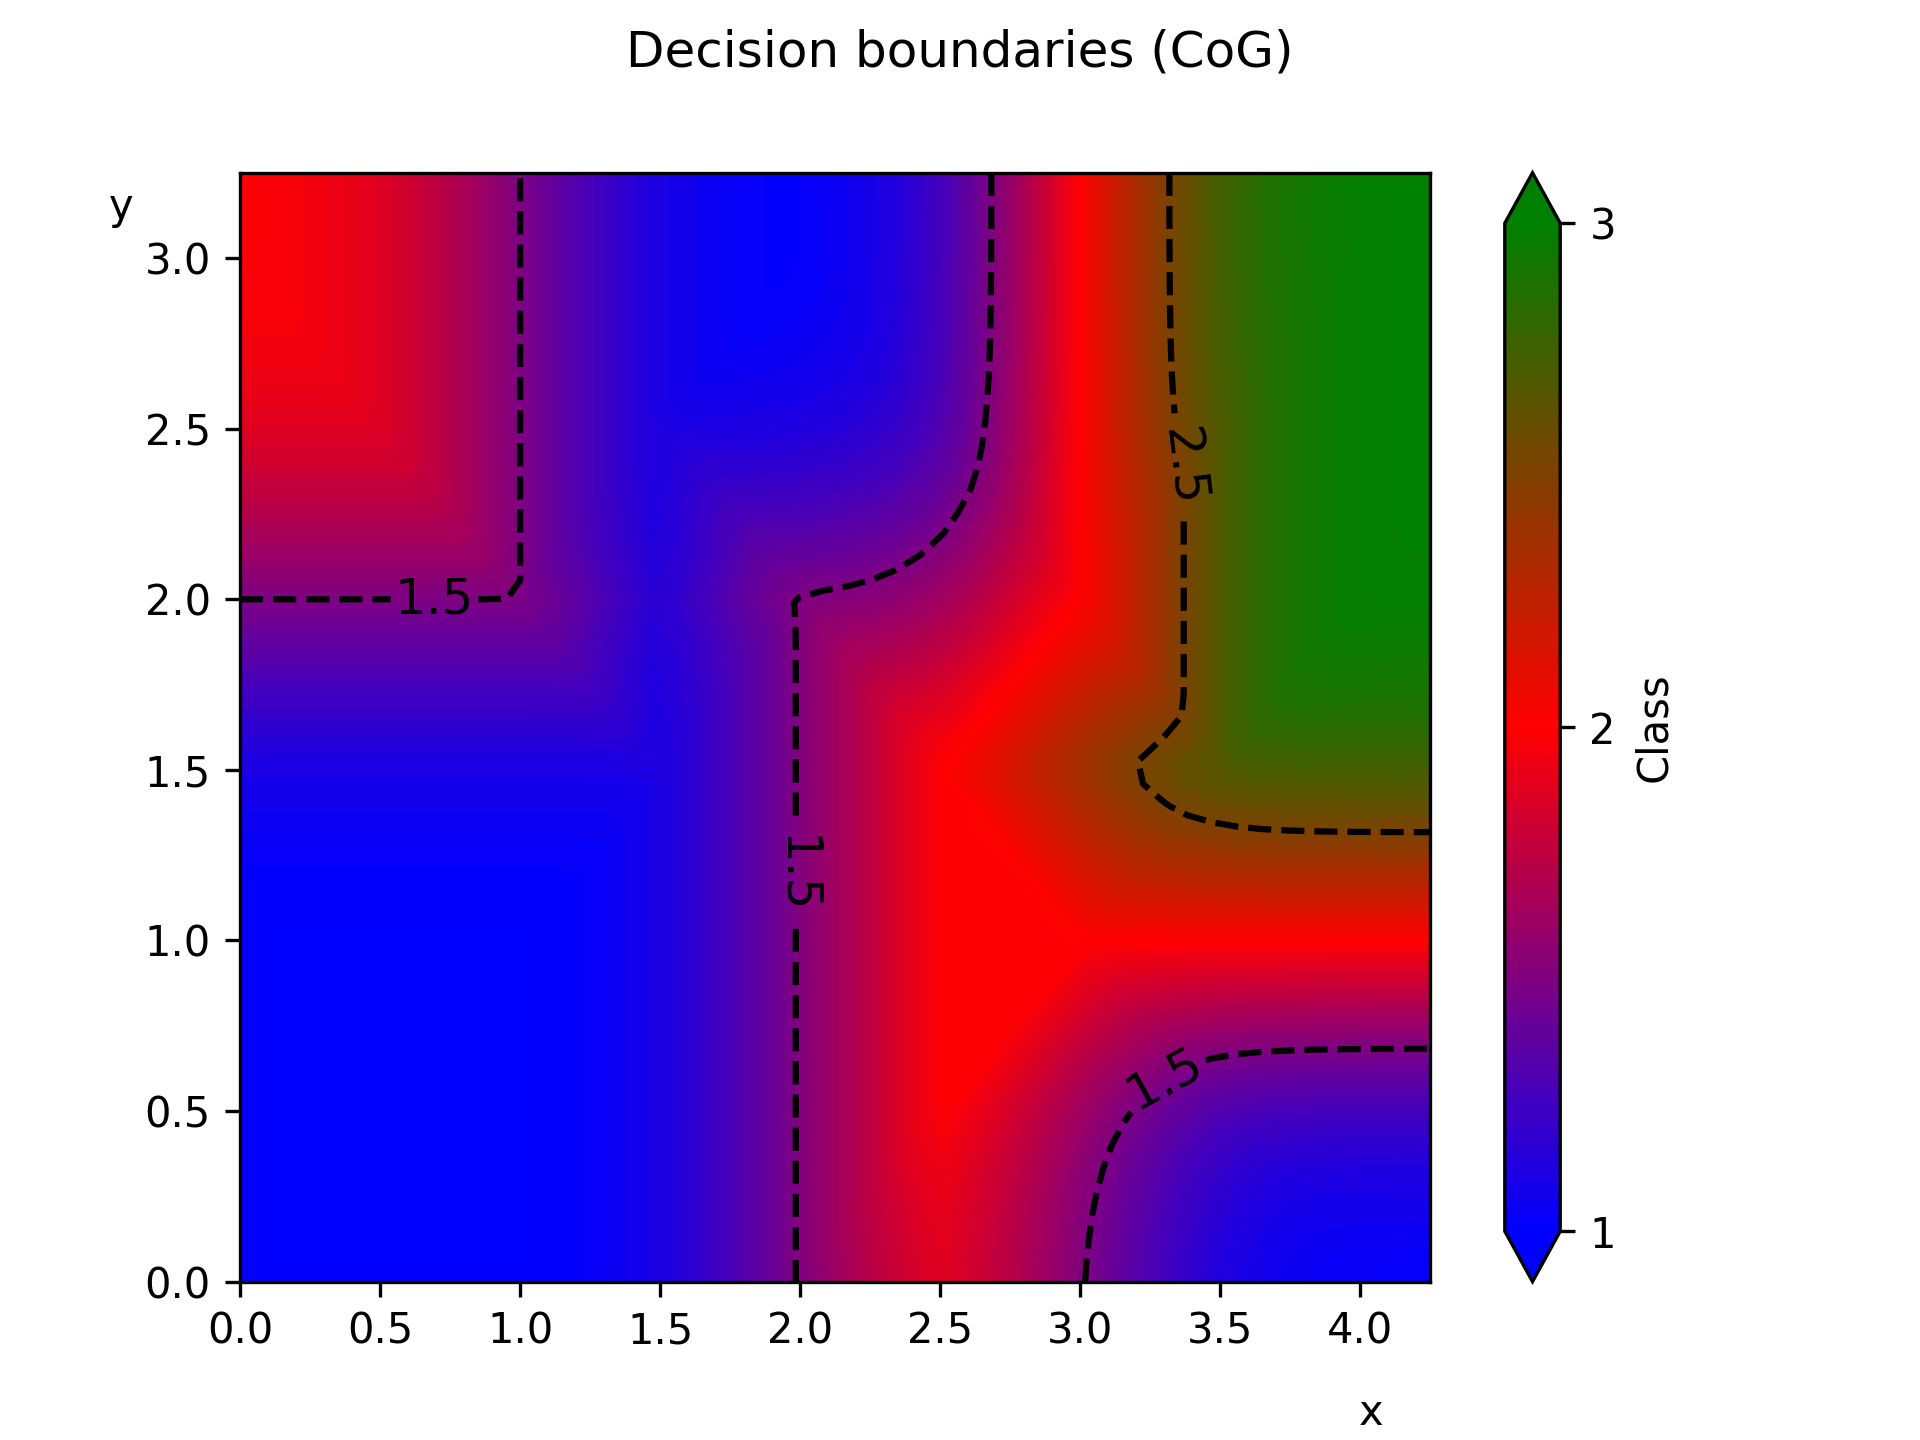
\includegraphics[width=\textwidth,trim={0 0 0 1.25cm},clip]{figures/ProofOfConcepts/fuzzy_system_cog.png}};
            \begin{scope}[x={(image.south east)},y={(image.north west)}]
                \draw[yellow, thin,rounded corners] (.58,.67) rectangle (.70,.95);
                \draw[yellow, thin,rounded corners] (.65,.32) rectangle (.79,.48);
                \node (A) at (.55,.56) [yellow, anchor=east] {\tiny{Interpolation Error}};

                \draw[yellow, arrow] (A) -- (.58,.67);
                \draw[yellow, arrow] (A) -- (.65,.48);
            \end{scope}
        \end{tikzpicture}
        \caption[Decision surface of the fuzzy rules using COG method]{Decision surface when using the COG method. The highlighted areas show interpolation errors.}
        \label{fig:fuzzyDecisionSurfaceExampleCOG}
    \end{subfigure}
    \hfill
    \begin{subfigure}[t]{0.45\textwidth}
        \centering
        \begin{tikzpicture}
            \node[anchor=south west,inner sep=0] (image) at (0,0) { 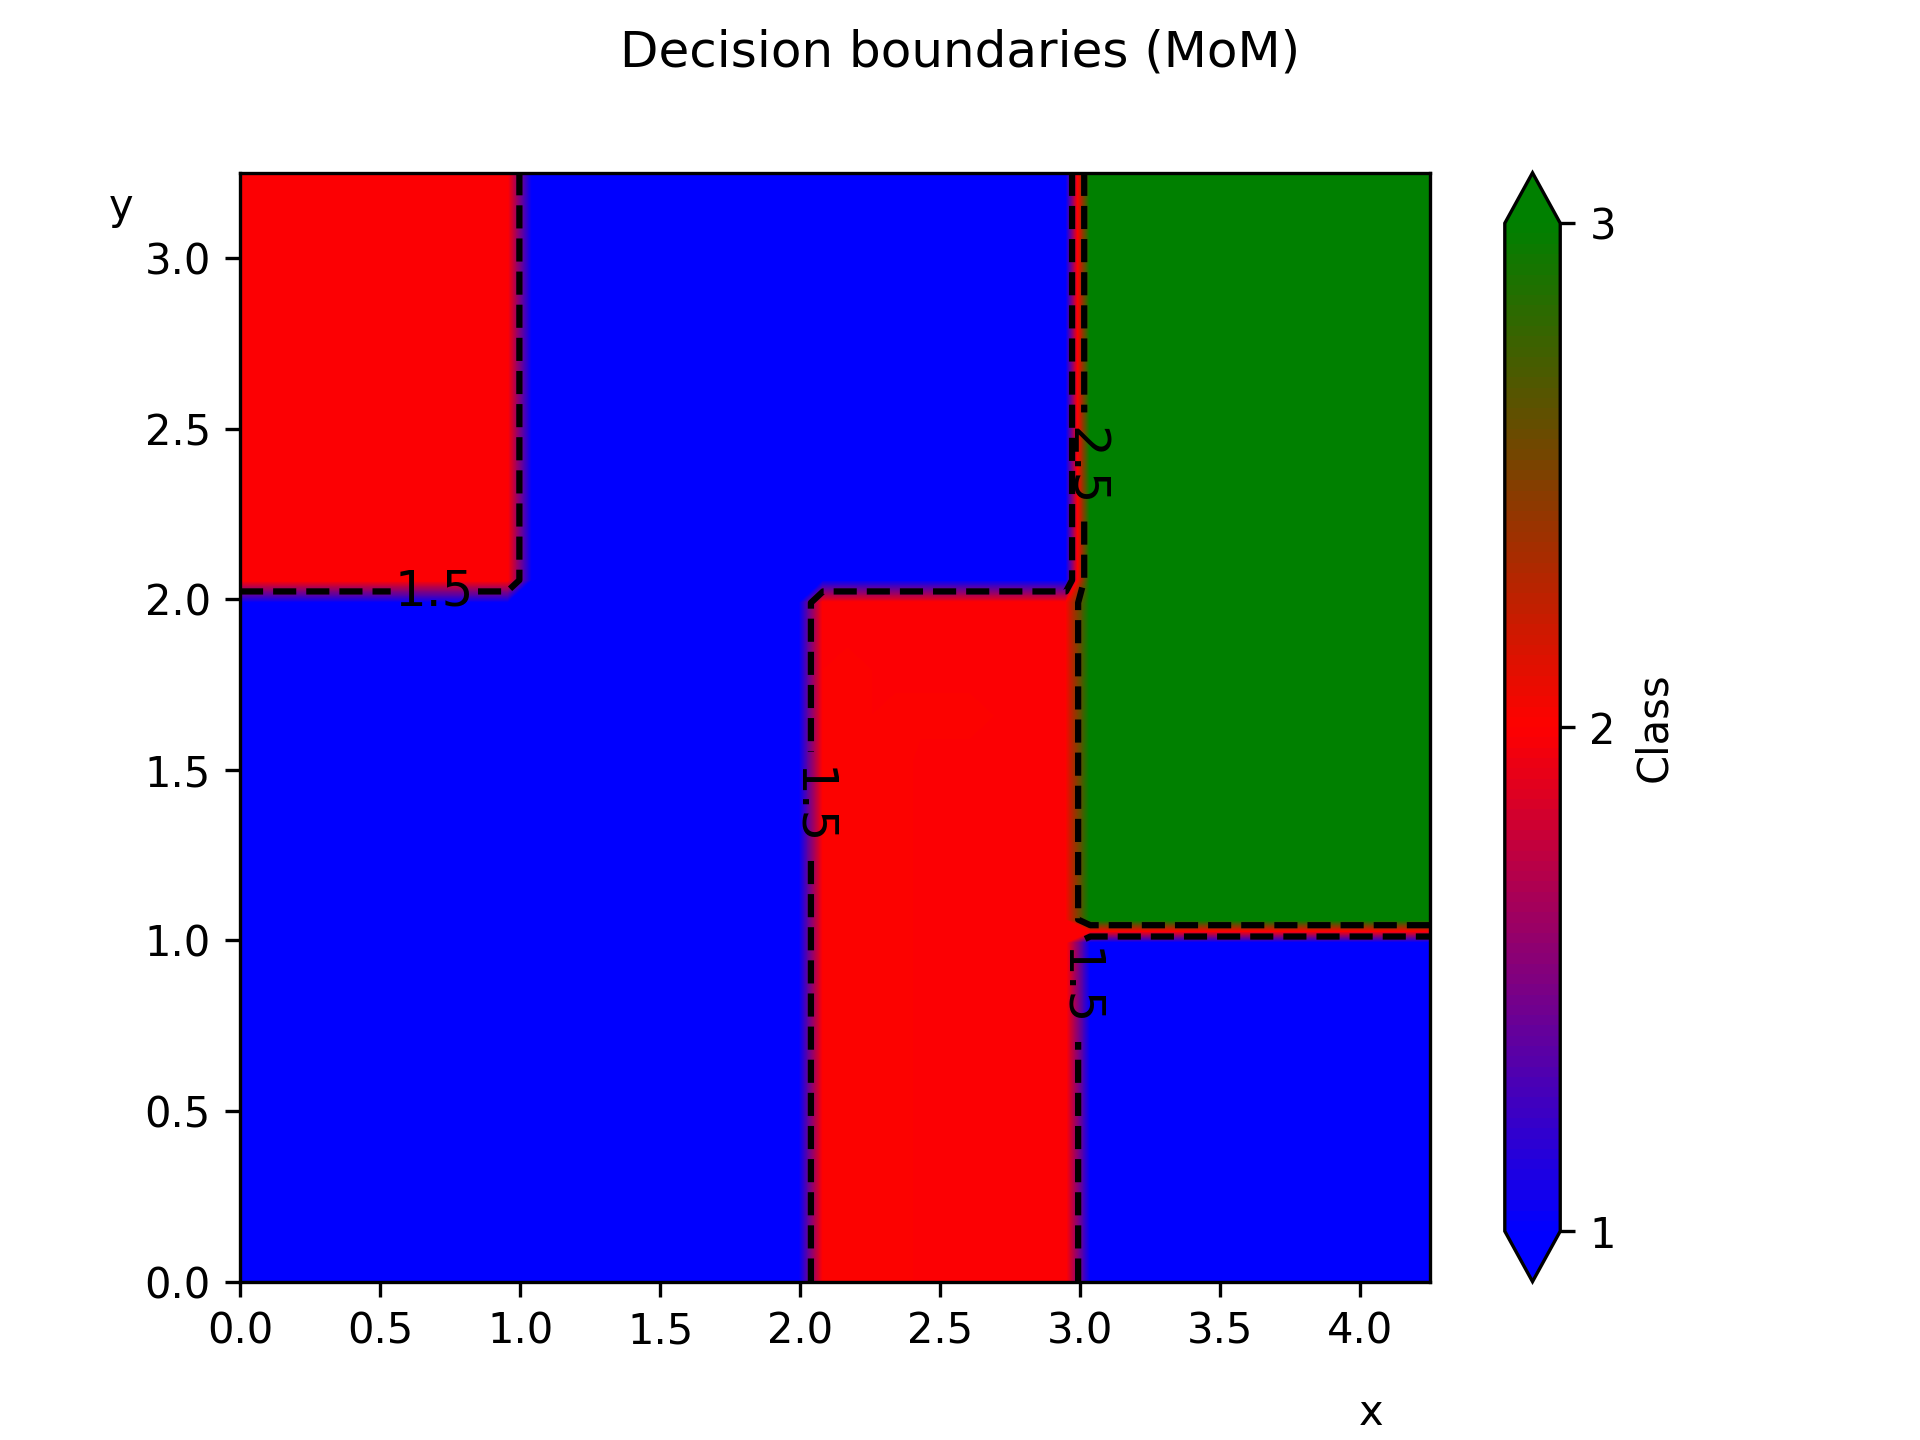
\includegraphics[width=\textwidth,trim={0 0 0 1.25cm},clip]{figures/ProofOfConcepts/fuzzy_system_mom.png}};
        \end{tikzpicture}
        \caption[Decision surface of the fuzzy rules using MOM method]{Decision surface when using the MOM method. There are only minor invalid regions in the decision surface.}
        \label{fig:fuzzyDecisionSurfaceExampleMOM}
    \end{subfigure}
    \caption{Comparison of COG and MOM decision surfaces of the fuzzy rules.}
    \label{fig:fuzzyDecisionSurfaceComparison}
\end{figure}


\section{Fuzzy Systems for \texttt{md\_flexible}}

This section will use the data-driven approach introduced in the previous section to demonstrate how to generate fuzzy systems for \texttt{md\_flexible} simulations. The first section will describe the data collection process needed to train the classic decision trees, and the later sections will use the obtained data to generate the two different styles of fuzzy systems introduced in \autoref{sec:fuzzyTuningStrategy}.

\subsection{Data Collection}

\subsubsection{Included Scenarios}

We chose to include the prominent example scenarios provided by \texttt{md\_flexible} such as \href{https://github.com/AutoPas/AutoPas/blob/c25dc770f173ff160630d7e58f59b38e277032a1/examples/md-flexible/input/fallingDrop.yaml}{\color{blue}\texttt{fallingDrop.yaml}}, \href{https://github.com/AutoPas/AutoPas/blob/c25dc770f173ff160630d7e58f59b38e277032a1/examples/md-flexible/input/explodingLiquid.yaml}{\color{blue} \texttt{explodingLiquid.yaml}} and \href{https://github.com/AutoPas/AutoPas/blob/c25dc770f173ff160630d7e58f59b38e277032a1/examples/md-flexible/input/SpinodalDecomposition.yaml}{\color{blue} \texttt{SpinodalDecomposition.yaml}} as the primary source of data. Additionally, we included some simulations of uniform cubes with different densities and particle counts to gather more data about the performance of the different configurations under lab-like conditions.

All simulations were run on the serial partition of the CoolMUC-2 cluster\textsuperscript{\ref{CoolMucSpecs}} and were repeated twice to account for fluctuations in performance. Furthermore, every simulation was repeated with 1, 4, 12, 24, and 28 threads to additionally gather data on how parallelization affects the ideal configuration.

All the values were collected with the newly created \texttt{PAUSE\_SIMULATION\_DURING\_TUNING} CMake option to ensure that the simulation state does not change during the tuning phases. This guarantees a fair comparison of the tested configurations, as all of them are evaluated under the exact same conditions. To gather the maximal amount of data, we used the \texttt{FullSeach} tuning strategy, which executes all possible configurations during the tuning phases.


\subsubsection{Collected Parameters}

The existing \texttt{TuningDataLogger} and the newly created \texttt{LiveInfoLogger} classes of the AutoPas framework allow us to collect a wide variety of parameters during the simulation, such as the used configuration, information about the state of the simulation, and the measured timing data for each iteration of the simulation.

The complete shape of the collected data can be found in \autoref{des:tuningdatafields} and \autoref{des:liveinfodatafields}, respectively. We will however only make use of a subset of the available LiveInfo data, as we are only interested in \emph{relative} values that do not change when the simulation is scaled up or down and are therefore primarily interested in: \texttt{avgParticlesPerCell}, \texttt{maxParticlesPerCell}, \texttt{homogeneity}, \texttt{maxDensity}, \texttt{particlesPerCellStdDev} and \texttt{threadCount}. This focus should help the fuzzy systems generalize better to unseen data, as they are less likely to overfit the training data.


\subsubsection{Limitations}

As the performance of machine learning models may degrade quickly when confronted with significantly different data than the data they were trained on, it is essential to collect a wide variety of scenarios to cover as many possible use cases as possible. As we only included a limited number of scenarios, we have to keep in mind that the generated fuzzy systems will only be able to make confident predictions about scenarios similar to the included ones, and we should not expect them to generalize well to unseen data.
To guarantee a fair evaluation of this tuning approach, we will only focus on slight variations of the included scenarios during the later evaluation phase in \autoref{sec:comparison_and_evaluation}.

\subsection{Data Preprocessing}

In order to make predictions about the performance of different configurations, we first need to define an appropriate metric to compare them. As we \emph{paused} the simulation during the tuning process with the \texttt{PAUSE\_SIMULATION\_DURING\_TUNING} option, we can safely use the runtimes of the different configurations to compare them. Those runtimes are, however, absolute values and may differ significantly between tuning phases as the underlying simulation changes. To compare runtimes between different tuning phases, we introduce the concept of \emph{relative speed}, which measures how well a configuration performs compared to the best configuration in the same tuning phase, and augment the collected timing data with this metric. The relative speed is calculated as


\begin{equation}
    {\text{relative speed}^{(i)}_{\text{config}}}= \frac{t_{\text{best}}^{(i)}}{t_{\text{config}}^{(i)}}
\end{equation}

Where $t_{\text{best}}^{(i)}$ is the runtime of the best configuration during the $i$-th tuning phase and $t_{\text{config}}^{(i)}$ is the runtime of the configuration we are interested in.

This value will range from 0 (being infinitely worse than the best configuration) to 1 (being equally good as the best configuration) for each configuration. Additionally, we chose to combine the fields \texttt{Container} and \texttt{DataLayout} of the configuration into a single field \texttt{ContainerDataLayout} as they are closely related and should be tuned together.

\medskip

\autoref{tab:trainingData} shows the augmented dataset for creating the fuzzy systems. The next sections sections will describe how this dataset can be used to create fuzzy systems for the so-called \emph{Component Tuning Approach} and the \emph{Suitability Tuning Approach}.


\definecolor{LightCyan}{rgb}{0.88,1,1}
\newcolumntype{g}{>{\columncolor{LightCyan}}c}
\begin{table}[H]
    \centering
    \tiny
    \def\arraystretch{2.5}
    \begin{tabular}{|c|c|c|c|c|c|c|c|c| g|}
        \cline{1-9}
        \multicolumn{3}{|c|}{ \textbf{ParticlesPerCell}} & \multicolumn{3}{c|}{\textbf{Miscellaneous}} & \multicolumn{3}{c|}{\textbf{Configuration}}                                                                                                                           \\
        \hline
        \textbf{avg}                                     & \textbf{max}                                & \textbf{stddev}                             & \tabularCenterstack{c}{\textbf{homo-}                                                                                   \\ \textbf{genity}} & \tabularCenterstack{c}{\textbf{max-} \\ \textbf{density}} & \textbf{threads} & \tabularCenterstack{c}{\textbf{Container} \\ \textbf{DataLayout}}& \textbf{Traversal} & \textbf{Newton3} & \tabularCenterstack{c}{\textbf{Relative} \\ \textbf{Speed}} \\
        \hline
        0.905                                            & 23                                          & 0.0129                                      & 0.0354                                & 0.531  & 1      & LinkedCells\_AoS      & lc\_sliced      & enabled  & 0.450641 \\
        2.201                                            & 13                                          & 0.0144                                      & 0.0861                                & 0.627  & 24     & VerletListsCells\_AoS & vlc\_sliced     & disabled & 0.594117 \\
        0.905                                            & 18                                          & 0.0136                                      & 0.0431                                & 0.319  & 4      & LinkedCells\_AoS      & lc\_sliced\_c02 & enabled  & 0.454632 \\
        \vdots                                           & \vdots                                      & \vdots                                      & \vdots                                & \vdots & \vdots & \vdots                & \vdots          & \vdots   & \vdots   \\
        \hline
    \end{tabular}
    \caption[Augmented dataset used for creating the fuzzy systems in \texttt{md\_flexible}
    ]{Augmented dataset used for creating the fuzzy systems. The dataset contains all collected parameters and the relative speed of the configuration compared to the best configuration in the same tuning phase.}
    \label{tab:trainingData}
\end{table}



\subsection{Component Tuning Approach}

This approach makes use of three different \texttt{FuzzySystems}, one for each of the tunable parameters of the simulation (\texttt{ContainerDataLayout}, \texttt{Traversal}, and \texttt{Newton3}). All those systems should independently predict the best configuration for their respective parameter based on the current LiveInfoData. \autoref{fig:fuzzySystemComponent} shows the structure of this approach.

As we only want to create a fuzzy system predicting good-performing configurations, we naively remove all configurations performing worse than a certain suitability threshold (we chose 70\%) as depicted in \autoref{fig:relativeSpeed}. The remaining configurations, which are known to perform well, are then used to create the fuzzy systems.


\begin{figure}[H]
    \centering
    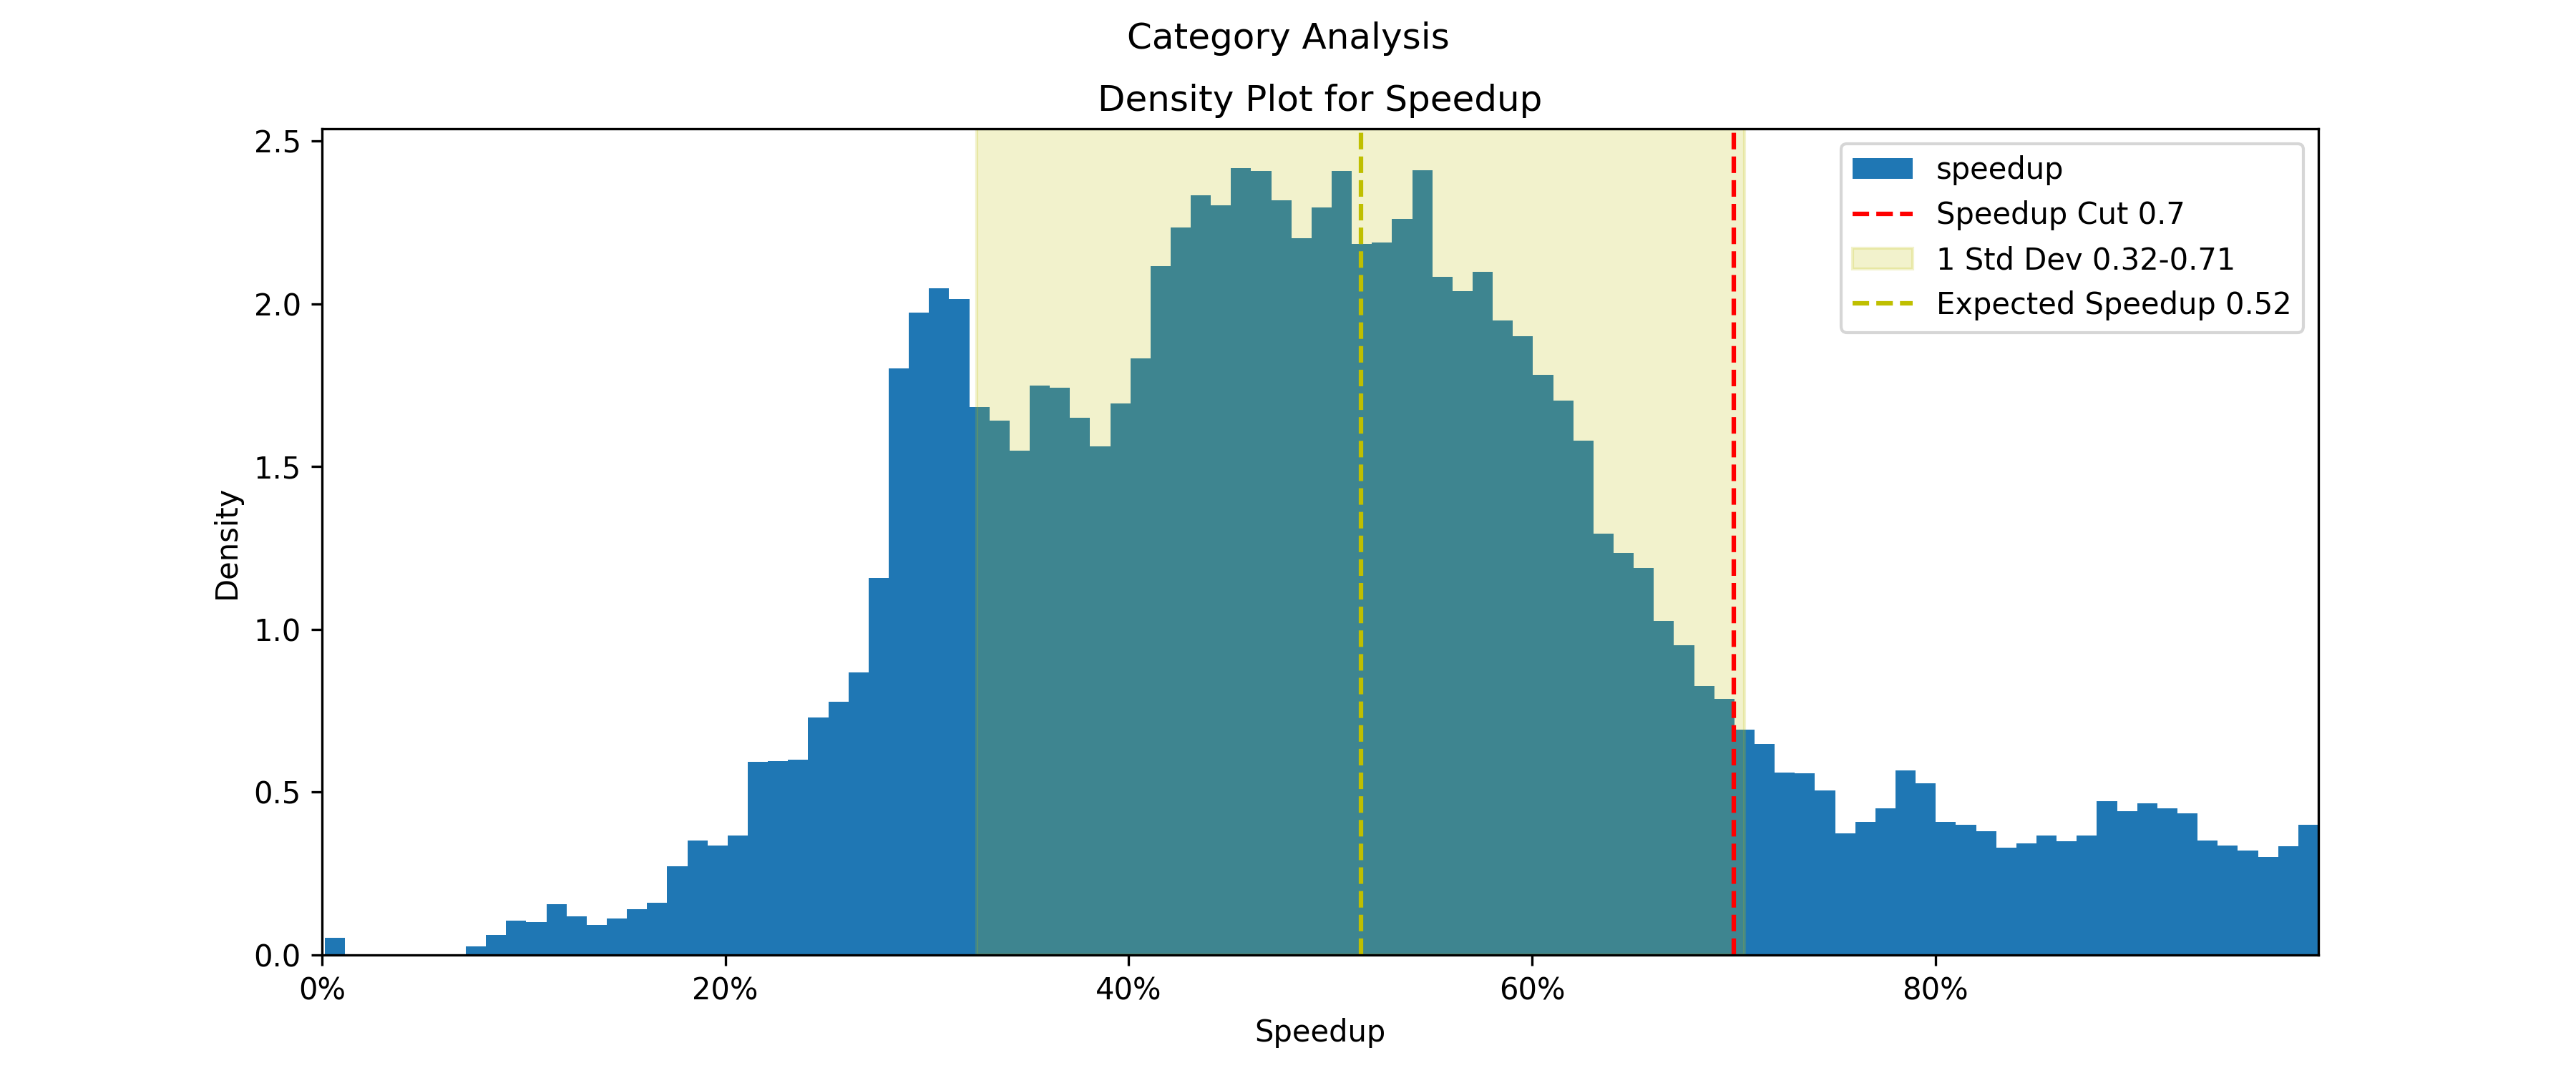
\includegraphics[width=\columnwidth,trim={1cm 0 2cm 1.5cm},clip]{figures/DataAnalytics/speedup.png}
    \caption[Relative speed distribution of the collected data]{Relative speed distribution of the collected data. The suitability threshold is set to 70\%, thus removing all configurations performing worse than this threshold. From the plot, we can also see that the average configuration performs just 52\% as well as the best configuration, with some configurations also performing ten times worse than the best in certain tuning phases.}
    \label{fig:relativeSpeed}
\end{figure}

Afterward, we group all configurations evaluated in the same tuning phase and aggregate all the present values of tunable parameters into a single term. As we \emph{paused} the simulation during the tuning phase, the LiveInfoData will be equal for such configurations, and the aggregated terms will therefore represent all \emph{good} values for the parameters in this simulation state (as they occur in configurations with $\geq 70\%$ suitability). The aggregated training data is shown in \autoref{tab:trainingDataComponent} and is used to fit three decision trees, which are then converted into fuzzy systems using the method described in the previous section. A few of the extracted fuzzy rules are shown in \autoref{tab:fuzzyRulesComponent}.

\begin{table}[H]
    \centering
    \tiny
    \def\arraystretch{2.5}
    \begin{tabular}{|c|c|c|c|c|c|c|c|c|}
        \cline{1-9}
        \multicolumn{3}{|c|}{ \textbf{ParticlesPerCell}} & \multicolumn{3}{c|}{\textbf{Miscellaneous}} & \multicolumn{3}{c|}{\textbf{Aggregated Configuration Terms}}                                                                                                                               \\
        \hline
        \textbf{avg}                                     & \textbf{max}                                & \textbf{stddev}                                              & \tabularCenterstack{c}{\textbf{homo-}                                                                                       \\ \textbf{genity}} & \tabularCenterstack{c}{\textbf{max-} \\ \textbf{density}} & \textbf{threads} & \tabularCenterstack{c}{\textbf{Container} \\ \textbf{DataLayout}}& \textbf{Traversal} & \textbf{Newton3}  \\
        \hline
        0.906                                            & 15                                          & 0.015                                                        & 0.055                                 & 0.297  & 4      & \tabularCenterstack{c}{"LinkedCells\_SoA,                         \\ VerletClusterLists\_SoA, \\ VerletListsCells\_AoS"} & \tabularCenterstack{c}{"lc\_sliced, \\ lc\_sliced\_balanced, \\ lc\_sliced\_c02"} & "enabled"   \\
        \hline
        0.945                                            & 25                                          & 0.041                                                        & 0.084                                 & 0.673  & 24     & \tabularCenterstack{c}{"LinkedCells\_SoA,                         \\ VerletClusterLists\_SoA, \\ VerletListsCells\_AoS"} & \tabularCenterstack{c}{"lc\_c04, \\ lc\_c08, \\ lc\_sliced, \\ lc\_sliced\_balanced"} & \tabularCenterstack{c}{"disabled, \\ enabled"}  \\
        \hline
        0.906                                            & 20                                          & 0.014                                                        & 0.041                                 & 0.336  & 24     & \tabularCenterstack{c}{VerletClusterLists\_SoA,                   \\ VerletListsCells\_AoS} & \tabularCenterstack{c}{"vcl\_c06, \\ vlc\_c01, \\ vlc\_c18"} & \tabularCenterstack{c}{"disabled, \\ enabled"} \\
        \hline
        \vdots                                           & \vdots                                      & \vdots                                                       & \vdots                                & \vdots & \vdots & \vdots                                          & \vdots & \vdots \\
        \hline
    \end{tabular}
    \caption[Aggregated training data for the Component Tuning Approach]{Aggregated training data for the Component Tuning Approach. Each row represents a different tuning phase. The numerical values stem from the LiveInfoData during that tuning phase, and the aggregated configuration terms represent the configuration options that are known to perform well under the given conditions.}
    \label{tab:trainingDataComponent}
\end{table}


\begin{table}[H]
    \footnotesize
    \centering
    \addtolength{\leftskip} {-3cm} % increase (absolute) value if needed
    \addtolength{\rightskip}{-3cm}

    \begin{tabular}{|c|c|c|c|g|}
        \multicolumn{4}{c}{\large{\textbf{Antecedent}}} & \multicolumn{1}{c}{\large{\textbf{Consequent}    }}                                                                                                                                    \\
        \hline
        \textbf{avgParticlesPC}                         & \textbf{homogeneity}                                & \textbf{particlesPCStdDev}                        & \textbf{threadCount}      & \textbf{ContainerDataLayout}                     \\

        \hline
        \texttt{lower than 3.45}                        & \texttt{lower than 0.05}                            &                                                   & \texttt{lower than 18.0}  & \tabularCenterstack{c}{"VerletClusterLists\_SoA, \\
        VerletListsCells\_AoS"}                                                                                                                                                                                                                  \\
        \hline
        \texttt{lower than 3.45}                        & \texttt{higher than 0.05}                           & \texttt{lower than 0.024}                         & \texttt{higher than 18.0} & \tabularCenterstack{c}{"LinkedCells\_SoA,        \\ VerletClusterLists\_SoA,\\ VerletListsCells\_AoS"}  \\
        \hline
        \vdots                                          & \vdots                                              & \vdots                                            & \vdots                    & \vdots                                           \\
        \hline

        \multicolumn{5}{c}{ }                                                                                                                                                                                                                    \\


        \multicolumn{4}{c}{\large{\textbf{Antecedent}}} & \multicolumn{1}{c}{\large{\textbf{Consequent}    }}                                                                                                                                    \\

        \hline
        \textbf{avgParticlesPC}                         & \textbf{homogeneity}                                & \textbf{particlesPCStdDev}                        & \textbf{threadCount}      & \textbf{Traversal}                               \\

        \hline

        \texttt{lower than 1.553}                       & \texttt{higher than 0.047}                          & \texttt{lower than 0.023	}                         & \texttt{higher than 2.5}  & \tabularCenterstack{c}{"lc\_sliced,              \\ vlc\_c18,\\ lc\_sliced\_c02"}
        \\
        \hline

                                                        & \texttt{lower than 0.037}                           & \texttt{lower than 0.023	}                         & \texttt{lower than 26.0}  & \tabularCenterstack{c}{"vcl\_c06,                \\ vlc\_c18,\\ vlc\_sliced\_c02"}                                                          \\


        \hline
        \vdots                                          & \vdots                                              & \vdots                                            & \vdots                    & \vdots                                           \\
        \hline


        \multicolumn{5}{c}{ }                                                                                                                                                                                                                    \\


        \multicolumn{4}{c}{\large{\textbf{Antecedent}}} & \multicolumn{1}{c}{\large{\textbf{Consequent}    }}                                                                                                                                    \\

        \hline
        \textbf{avgParticlesPC}                         & \textbf{homogeneity}                                & \textbf{particlesPCStdDev}                        & \textbf{threadCount}      & \textbf{Newton 3}                                \\

        \hline

                                                        &                                                     & \texttt{higher than 0.03}                         & \texttt{higher than 18.0} & \tabularCenterstack{c}{"disabled,                \\enabled"}
        \\
        \hline

                                                        &                                                     & \tabularCenterstack{c}{\texttt{higher than 0.023}                                                                                \\ $\land$ \texttt{lower than 0.037	}} &  \tabularCenterstack{c}{\texttt{lower than 18.0}\\ $\land$ \texttt{higher than 8.0	}} & \tabularCenterstack{c}{"enabled"}                \\


        \hline
        \vdots                                          & \vdots                                              & \vdots                                            & \vdots                    & \vdots                                           \\
        \hline
    \end{tabular}

    \caption[Selected fuzzy rules for the Component Tuning Approach]{Extracted fuzzy rules from the decision trees for the Component Tuning Approach. The rules are grouped by the tunable parameter they predict. The first row is read as:
        \footnotesize{$\text{IF} \;  (\text{avgParticlesPC} = \text{"lower than 3.454"})  \land   (\text{homogeneity} = \text{"lower than 0.05"})   \land (\text{threadCount} = \text{"lower than 18.0"}) \; \text{THEN} \; (\text{ContainerDataLayout} = \text{"VerletClusterLists\_SoA, VerletListsCells\_AoS"})$}}
    \label{tab:fuzzyRulesComponent}
\end{table}

\newpage

As described previously, we use \texttt{gaussian} membership functions for each linguistic term of the consequent linguistic variables. The exact placement of the values is irrelevant as we will use the MOM defuzzification method, but they should be chosen so that they do not overlap completely. \autoref{fig:homogenityLinguisticVariable} and \autoref{fig:newton3LinguisticVariable_component} show the resulting linguistic variables for the homogeneity linguistic variable (an input variable) and the Newton3 linguistic variable (an output variable). The visualizations of the other variables follow a similar pattern but are more complex due to the higher number of terms and are therefore not shown here.



\begin{figure}[H]
    \centering
    \begin{subfigure}{\columnwidth}
        \centering
        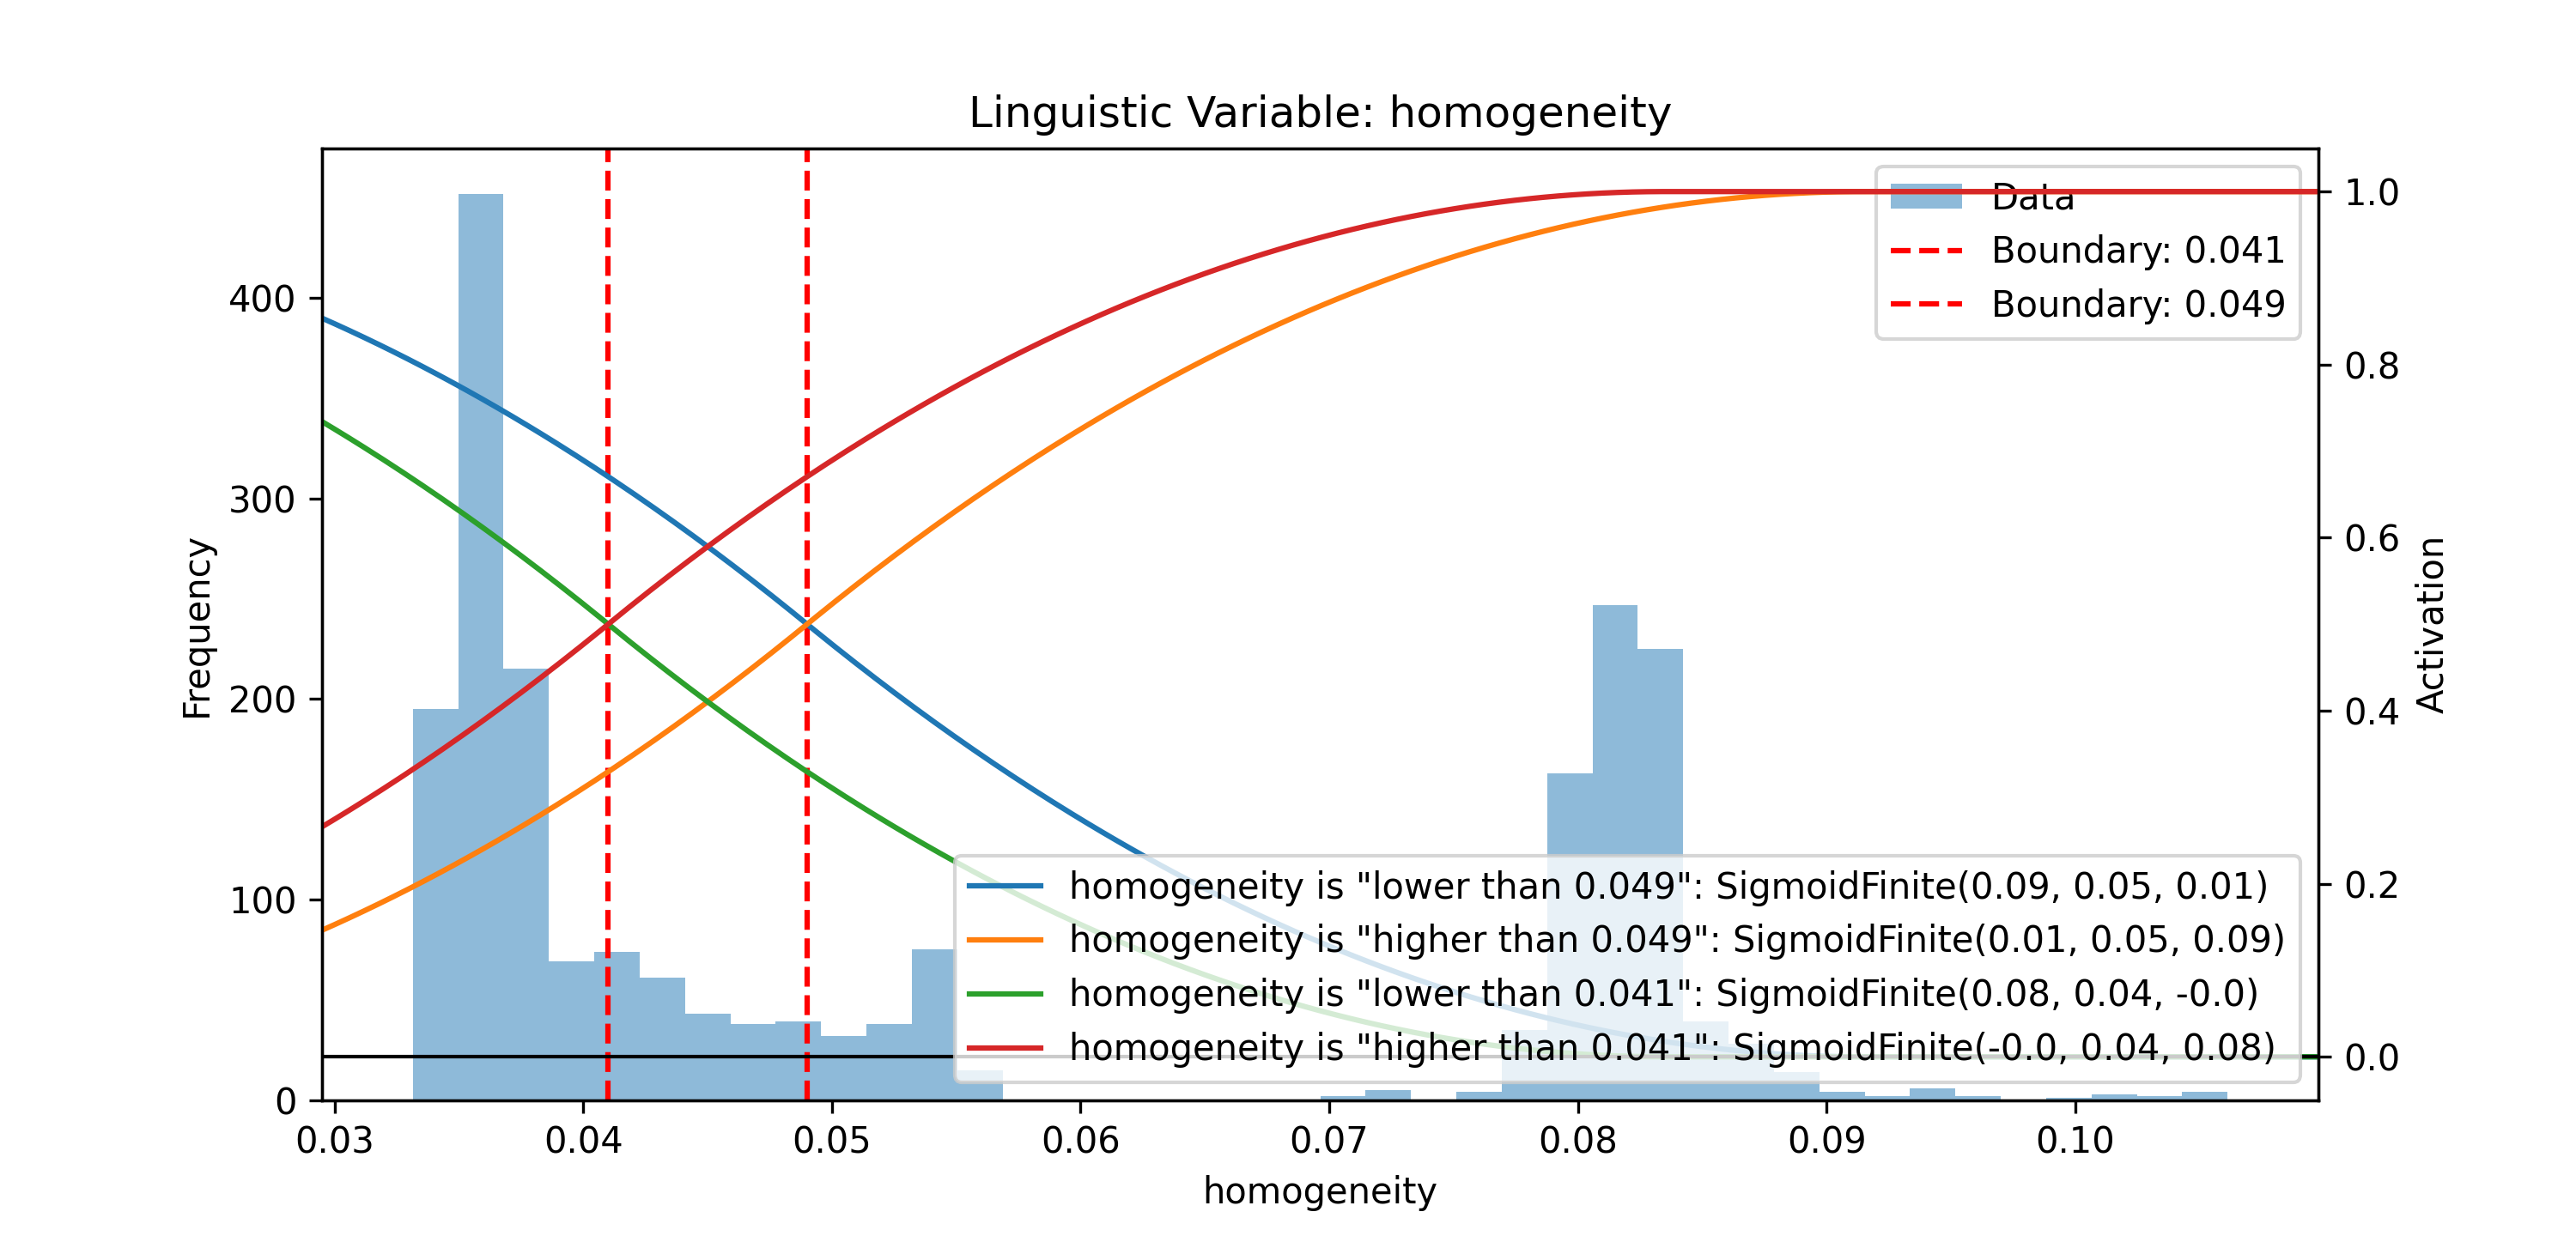
\includegraphics[width=0.8\textwidth,trim={1cm 0 1cm 1.35cm},clip]{figures/DataAnalytics/homogenity_linguistic_variable.png}
        \caption{Linguistic variable for the Homogeneity attribute}
        \label{fig:homogenityLinguisticVariable}
    \end{subfigure}
    \vspace{1cm}
    \begin{subfigure}{\columnwidth}
        \centering
        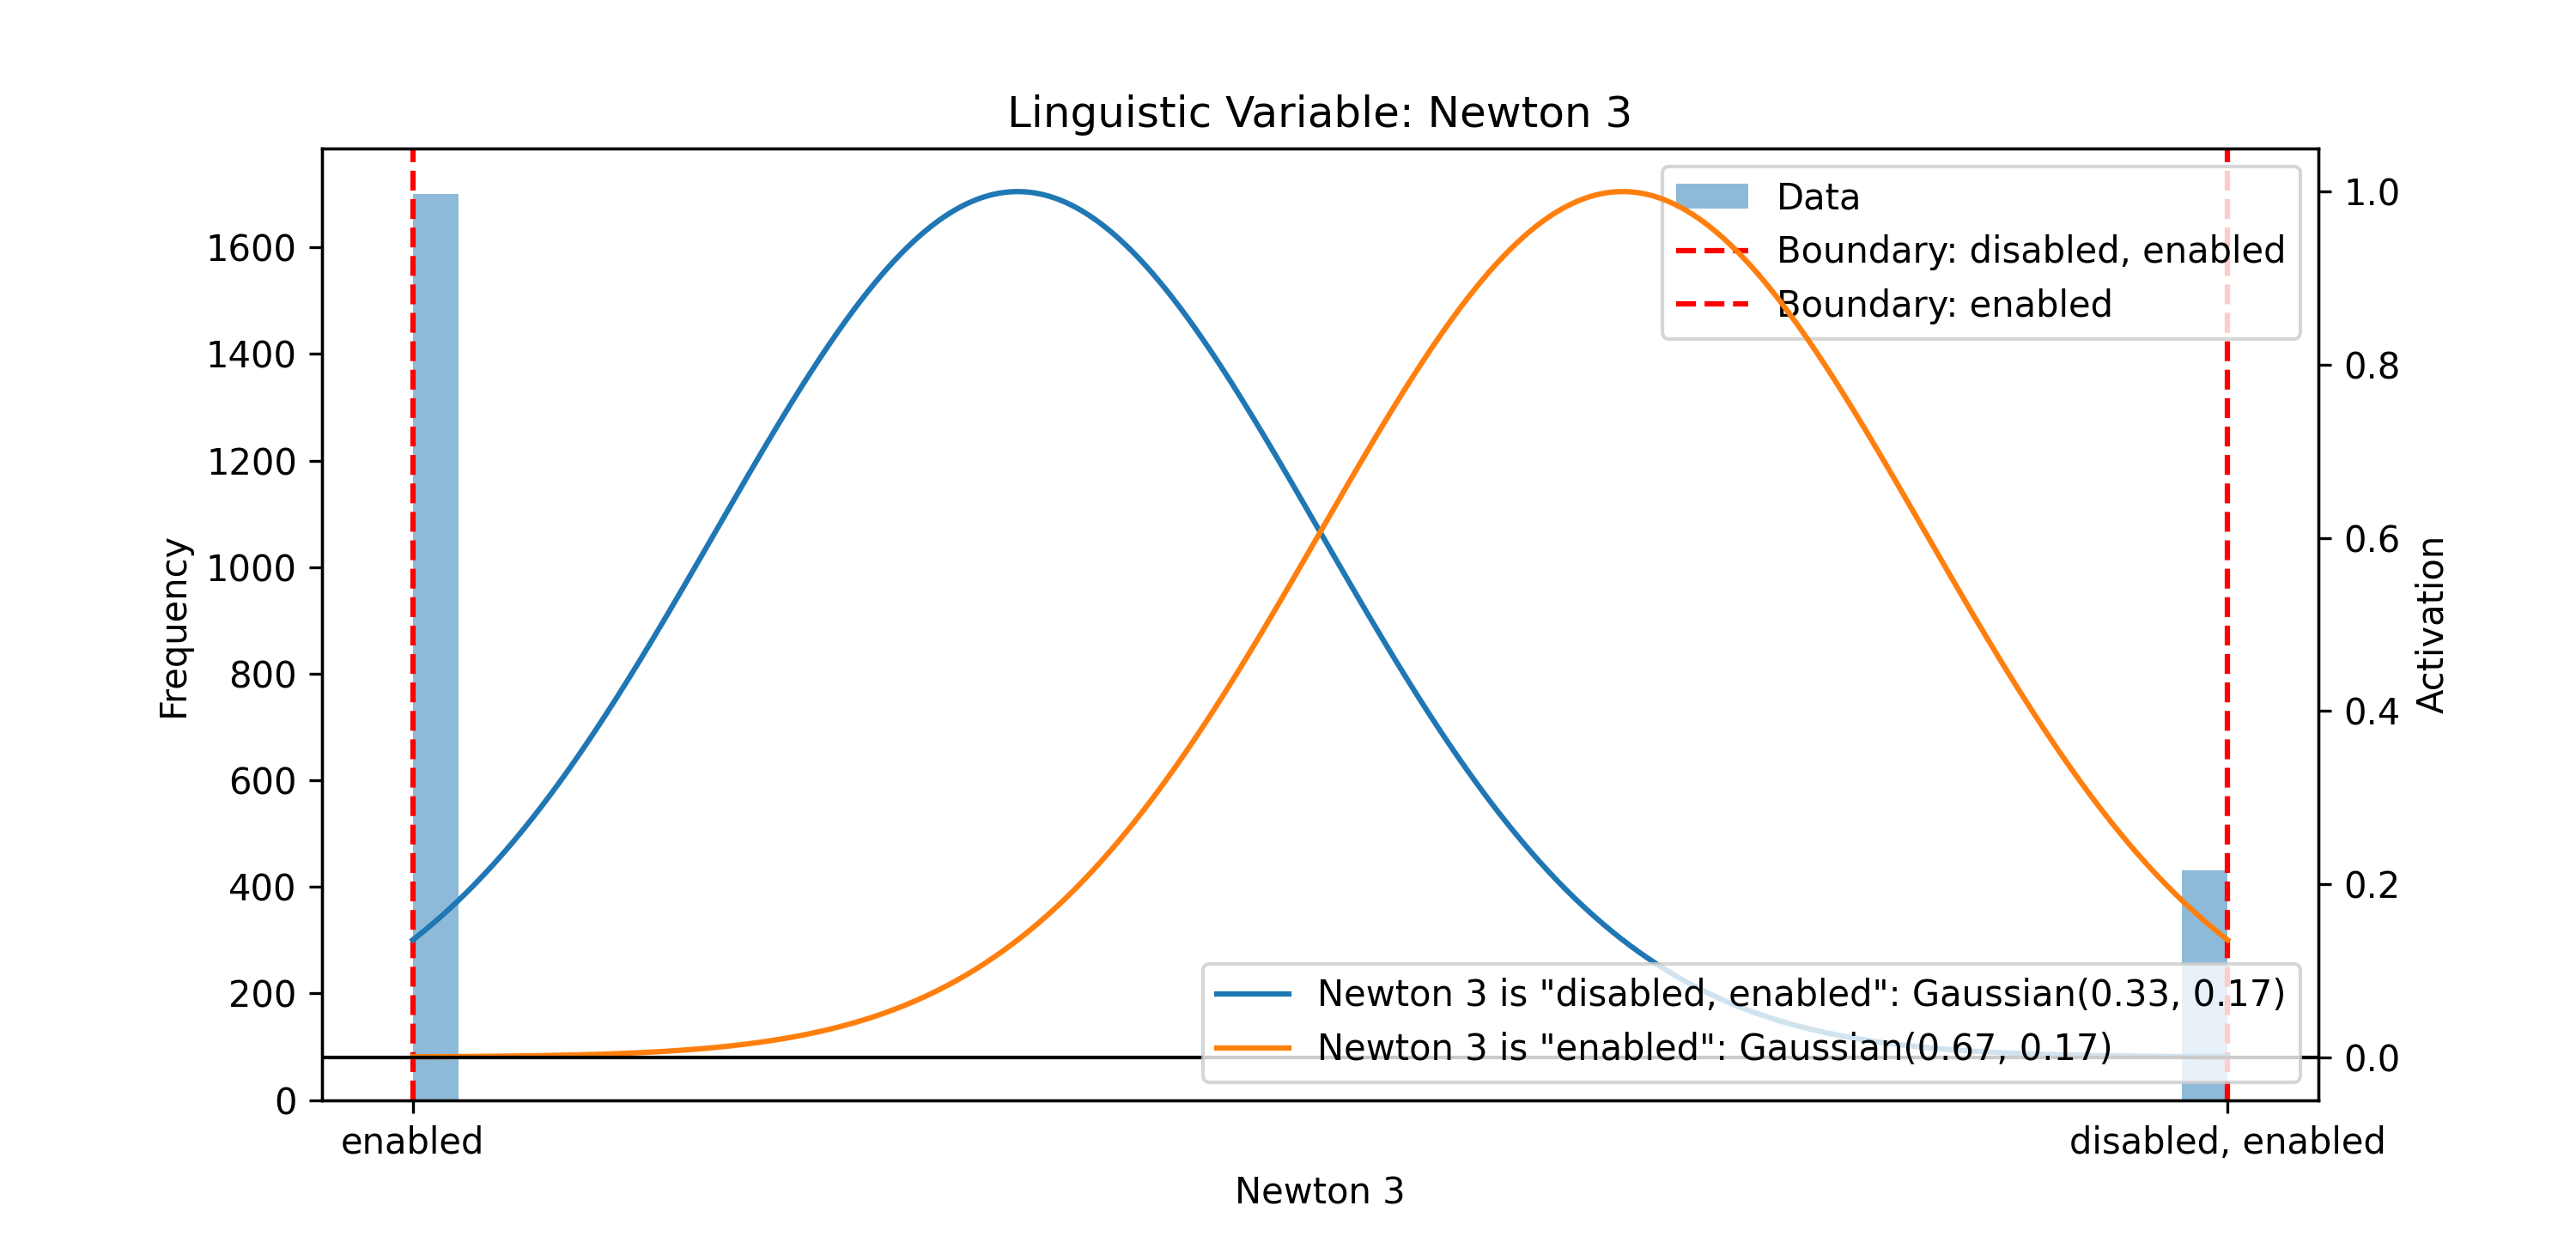
\includegraphics[width=0.8\textwidth,trim={1cm 0 1cm 1.35cm},clip]{figures/DataAnalytics/newton3_linguistic_variable.png}
        \caption{Linguistic variable for the Newton3 attribute}
        \label{fig:newton3LinguisticVariable_component}
    \end{subfigure}
    \caption{Linguistic variables for Homogeneity and Newton3 attributes. The background shows the histogram values present in the dataset.}
    \label{fig:linguisticVariables}
\end{figure}

\noindent These linguistic variables and fuzzy rules are then used to create the fuzzy systems for the component tuning approach. After creating a suitable OutputMapper, we construct the final rule file for the component tuning approach, which can be looked up at \href{https://github.com/AutoPas/AutoPas/blob/f77f10f72c19a86d5471bce287ae3a4ae344c012/examples/md-flexible/input/fuzzyRulesComponents.frule}{\color{blue}\texttt{fuzzyRulesComponents.frule}}.

\newpage

\subsection{Suitability Tuning Approach}

The suitability approach differs from the component tuning approach in that it tries to predict a configuration's numerical \emph{suitability} value under the current conditions. Therefore, each possible configuration is assigned a unique fuzzy system tailored to evaluate the suitability of its assigned configuration. \autoref{fig:fuzzySystemSuitability} shows the structure of this approach.

\smallskip

To train the decision trees, we again use a classification-based approach with the terms \texttt{terrible}, \texttt{poor}, \texttt{bad}, \texttt{medium}, \texttt{ok}, \texttt{good}, and \texttt{excellent} each corresponding to specific ranges of suitability values (see \autoref{fig:suitabilityClasses} for the exact placement). Conveniently, we can use $suitability = relative \ speed$, as the relative speed value already measures how well a configuration performs.

\smallskip

We create the training data for the decision trees by adding a new column to the aggregated training data containing the suitability class to which the numeric relative speed value mostly belongs. The final training data is shown in \autoref{tab:trainingDataSuitability}. After grouping the data by possible configurations, it is again possible to use these data points to train the decision trees and extract the fuzzy rules from them. Due to the grouping, each configuration receives a fuzzy system with rules explicitly tailored to it. Some resulting rules are shown in \autoref{tab:fuzzyRulesSuitability}.

\medskip

\noindent By again constructing corresponding linguistic variables and a suitable OutputMapper, we can create the final rule file for the suitability approach, which can be looked up at \href{https://github.com/AutoPas/AutoPas/blob/f77f10f72c19a86d5471bce287ae3a4ae344c012/examples/md-flexible/input/fuzzyRulesSuitability.frule}{\color{blue}\texttt{fuzzyRulesSuitability.frule}}.

\begin{figure}[H]
    \centering
    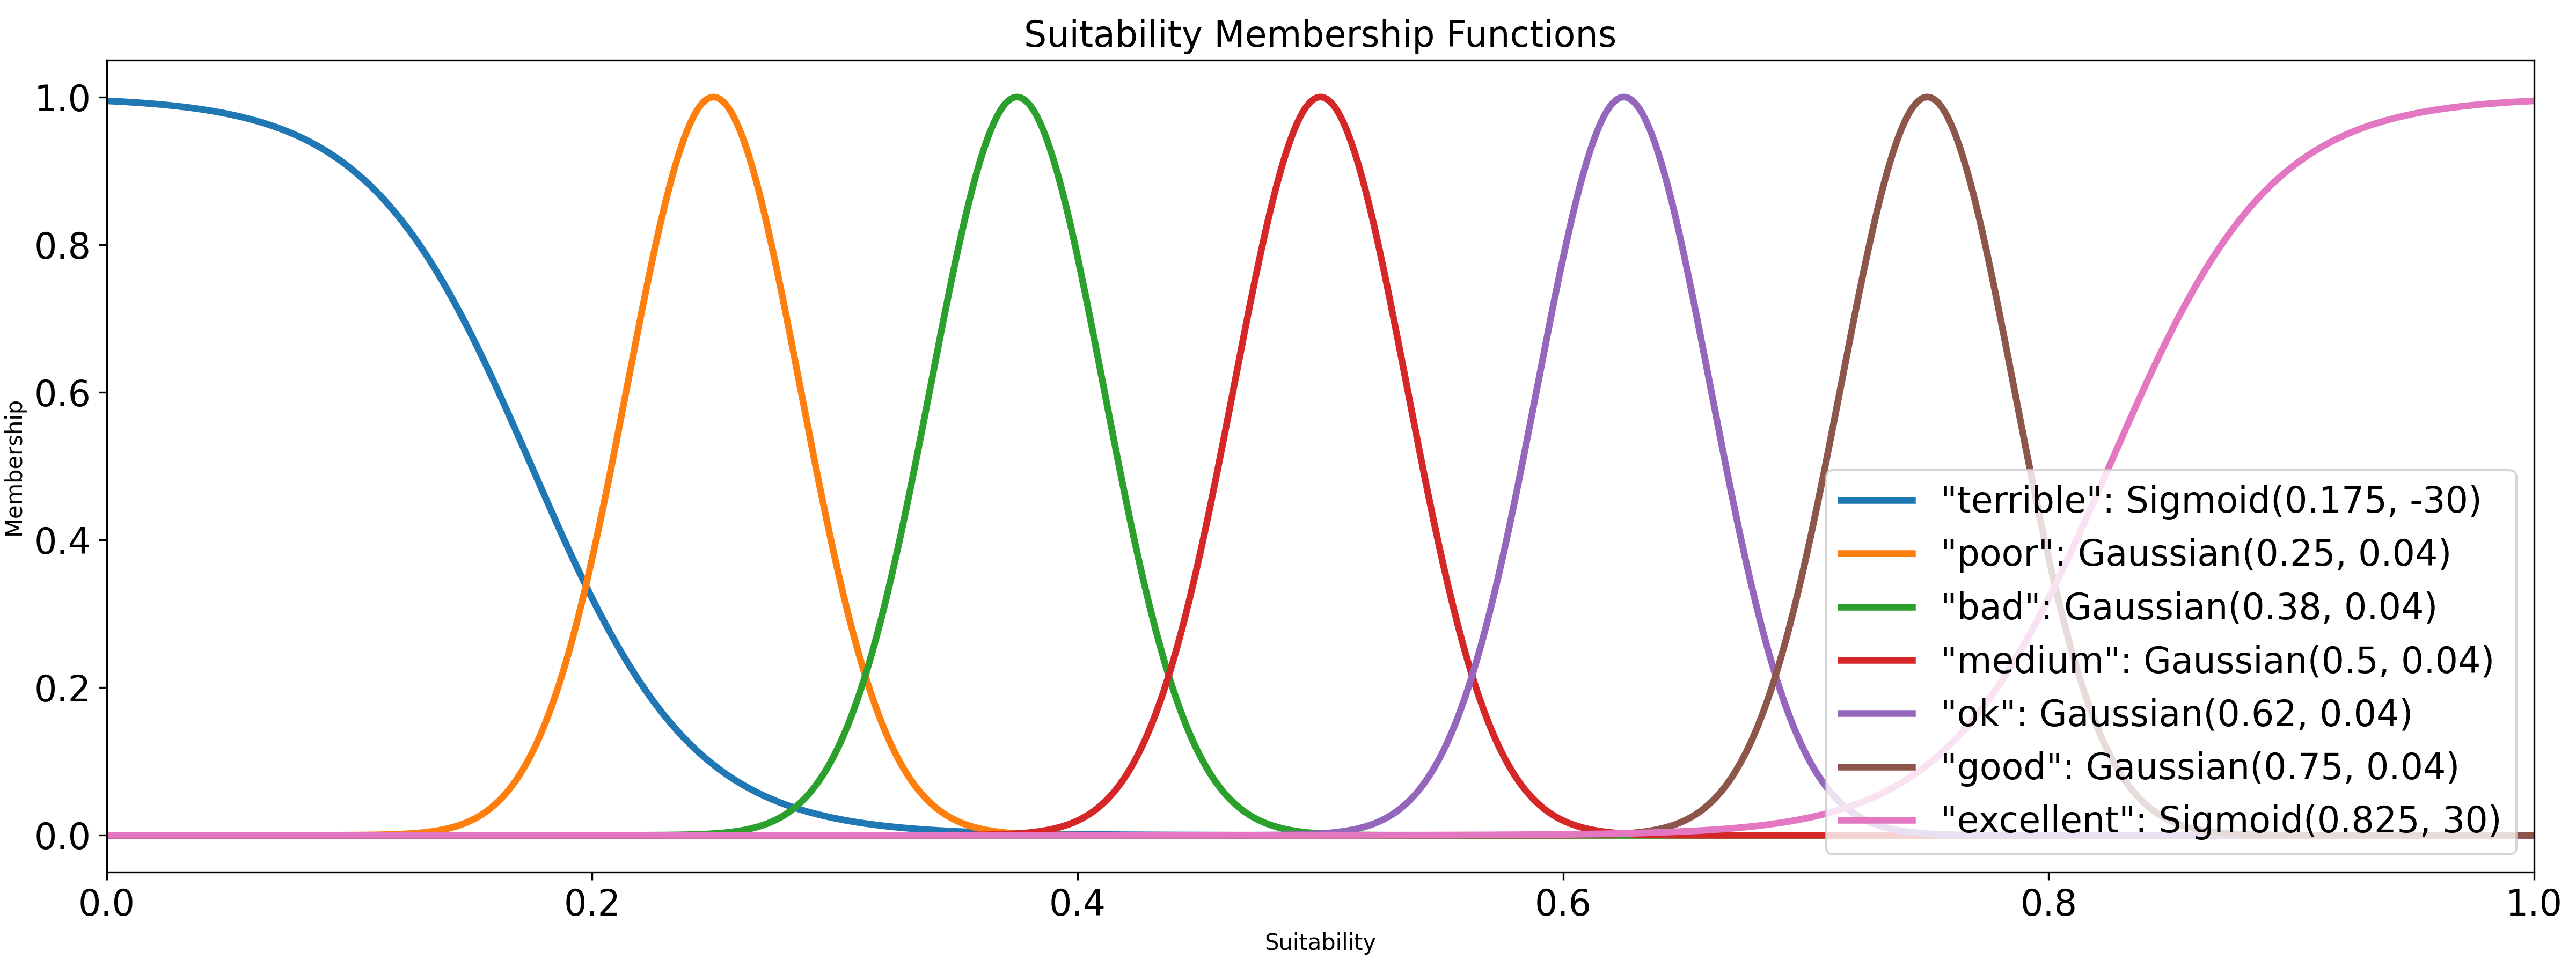
\includegraphics[width=\columnwidth,trim={0cm 0 0cm 0cm},clip]{figures/ProofOfConcepts/suitability_membership_functions.png}
    \caption[Linguistic variable for the Suitability attribute]{
        Linguistic variable for the Suitability attribute. The domain between 0\% suitability and 100\% suitability is divided into 7 classes: \texttt{terrible}, \texttt{poor}, \texttt{bad}, \texttt{medium}, \texttt{ok}, \texttt{good}, and \texttt{excellent}. The inner membership functions have a \texttt{gaussian} shape, while the outer ones have a \texttt{sigmoid} shape to capture the one-sided nature of those boundaries. The choice to use seven classes was made somewhat arbitrarily, with the intention to densely cover the range of suitability values with enough precision.
    }
    \label{fig:suitabilityClasses}
\end{figure}


\definecolor{LightRed}{rgb}{1,0.88,0.88}
\newcolumntype{u}{>{\columncolor{LightRed}}c}


\begin{table}[H]
    \centering
    \addtolength{\leftskip} {-3cm} % increase (absolute) value if needed
    \addtolength{\rightskip}{-3cm}
    \tiny
    \def\arraystretch{2.5}
    \begin{tabular}{|c|c|c|c|c|c|c|c|c|c|u|}
        \cline{1-9}
        \multicolumn{3}{|c|}{ \textbf{ParticlesPerCell}} & \multicolumn{3}{c|}{\textbf{Miscellaneous}} & \multicolumn{3}{c|}{\textbf{Configuration }}                                                                                                                                                            \\
        \hline
        \textbf{avg}                                     & \textbf{max}                                & \textbf{stddev}                              & \tabularCenterstack{c}{\textbf{homo-}                                                                                                                    \\ \textbf{genity}} & \tabularCenterstack{c}{\textbf{max-} \\ \textbf{density}} & \textbf{threads} & \tabularCenterstack{c}{\textbf{Container} \\ \textbf{DataLayout}}& \textbf{Traversal} & \textbf{Newton3}& \textbf{Relative speed}  & \textbf{Suitability}  \  \\
        \hline
        0.905                                            & 15                                          & 0.012                                        & 0.035                                 & 0.531  & 1      & LinkedCells\_AoS                              & lc sliced    & enabled  & 0.450  & "bad”       \\
        \hline
        0.944                                            & 25                                          & 0.012                                        & 0.083                                 & 0.691  & 28     & \tabularCenterstack{c}VerletClusterLists\_AoS & vcl\_c06     & disabled & 0.319  & "poor"      \\
        \hline
        0.944                                            & 20                                          & 0.012                                        & 0.079                                 & 0.041  & 12     & LinkedCell\_SoA                               & vlc\_ sliced & enabled  & 0.989  & "excellent" \\
        \hline
        \vdots                                           & \vdots                                      & \vdots                                       & \vdots                                & \vdots & \vdots & \vdots                                        & \vdots       & \vdots   & \vdots & \vdots      \\
        \hline
    \end{tabular}
    \caption[Prepared training data for the Suitability Approach]{Training data for the Suitability Approach. The dataset contains the LiveInfoData of the simulation, the current configuration, the relative speed, and the suitability values of the configuration. Each row represents a different configuration evaluated in a tuning phase.}
    \label{tab:trainingDataSuitability}
\end{table}





\begin{table}[H]
    \footnotesize
    \centering
    \addtolength{\leftskip} {-3cm} % increase (absolute) value if needed
    \addtolength{\rightskip}{-3cm}

    \begin{tabular}{|c|c|c|c|g|}
        \multicolumn{4}{c}{\large{\textbf{Antecedent}}} & \multicolumn{1}{c}{\large{\textbf{Consequent}    }}                                                                                                                                  \\
        \hline
        \textbf{avgParticlesPC}                         & \textbf{homogeneity}                                & \textbf{particlesPCStdDev} & \textbf{threadCount}                              & \tabularCenterstack{c} { \textbf{Suitability} \\ \textbf{ LinkedCells\_AoS} \\ \textbf{lc\_c01\_disabled}} \\

        \hline
                                                        & \texttt{lower than 0.084}                           & \texttt{higher than 0.029} & \texttt{higher than 26.0 }                        & "medium"                                      \\
        \hline
                                                        & \texttt{higher than 0.084}                          & \texttt{higher than 0.029} & \texttt{higher than 26.0 }                        & "bad"                                         \\
        \hline
                                                        &                                                     & \texttt{higher than 0.02}  & \texttt{lower than 2.5	 }                          & "poor"                                        \\

        \hline
        \vdots                                          & \vdots                                              & \vdots                     & \vdots                                            & \vdots                                        \\
        \hline

        \multicolumn{5}{c}{ }                                                                                                                                                                                                                  \\


        \multicolumn{4}{c}{\large{\textbf{Antecedent}}} & \multicolumn{1}{c}{\large{\textbf{Consequent}    }}                                                                                                                                  \\

        \hline
        \textbf{maxParticlesPerCell}                    & \textbf{homogeneity}                                & \textbf{particlesPCStdDev} & \textbf{threadCount}                              & \tabularCenterstack{c} { \textbf{Suitability} \\\textbf{ LinkedCells\_AoS}\\ \textbf{lc\_c04\_disabled}}\\

        \hline
        \texttt{higher than 18.5	}                       & \texttt{lower than 0.082}                           &                            & \tabularCenterstack{c} {\texttt{higher than 18.0}                                                 \\ $\land$ \texttt{ lower than 26.0}} & "medium" \\

        \hline
        \texttt{higher than 18.5	}                       & \texttt{higher than 0.082}                          &                            & \tabularCenterstack{c} {\texttt{higher than 18.0}                                                 \\ $\land$ \texttt{ lower than 26.0}} & "bad" \\
        \hline


        \vdots                                          & \vdots                                              & \vdots                     & \vdots                                            & \vdots                                        \\

        \hline
        \multicolumn{2}{c}{}                            & \multicolumn{1}{c}{\Huge{\vdots   }}                                                                                                                                                 \\
    \end{tabular}

    \caption[Selected fuzzy rules for the Suitability Approach]{Some extracted fuzzy rules from the decision trees for the Suitability Approach. The rules are grouped by the configuration they predict. The first row is read as:
        \footnotesize{$\text{IF} \;   (\text{homogeneity} = \text{lower than 0.084})   \land (\text{particlesPerCellStdDev} = \text{higher than 0.029})   \land (\text{threadCount} = \text{higher than 26.0}) \; \text{THEN} \; (\text{Suitability LinkedCells\_AoS\_lc\_c01\_disabled} = \text{"medium"})$}}
    \label{tab:fuzzyRulesSuitability}
\end{table}


\chapter{Comparison and Evaluation}
\label{sec:comparison_and_evaluation}

In this section, we compare the fuzzy tuning technique with other tuning techniques present in AutoPas and evaluate its performance.

To measure the performance of the fuzzy tuning strategy, we also use the scenarios present in \gls{mdflexible} and compare the results with the other tuning strategies present in AutoPas. The benchmarks are run on the CoolMUC-2\footnote{\label{CoolMucSpecs}CoolMUC-2 is a supercomputer located at the Leibniz Supercomputing Centre in Garching, Germany. It consists of 812 Haswell-based nodes with 14 cores each. As a result of hyperthreading, each node supports up to 28 threads. More information can be found at \url{https://doku.lrz.de/coolmuc-2-11484376.html}} cluster and are repeated with 1, 12, 24, and 28 threads. We use the \texttt{timeSpentCalculatingForces} metric to evaluate the performance of the tuning strategies as it gives a good indication of the overall performance of the simulation.


\section{Exploding Liquid Benchmark (Included in Training Data)}
\label{sec:explodingLiquidBenchmark}

The exploding liquid benchmark simulates a high-density liquid that expands outwards as the simulation progresses. As the data of this scenario was included in the training data, we expect the fuzzy tuning technique to perform well. We only include the benchmark results with one thread for brevity, as the results for the other thread counts are very similar.

The plot in \autoref{fig:explodingTimings_1thread} shows the time spent calculating the forces for each tuning strategy throughout the simulation. The fuzzy tuning strategies typically perform close to optimal and are very stable. All other tuning strategies show a much higher variance caused by testing many configurations during the tuning phases.

The low tuning overhead is the most significant contributor to the performance of the fuzzy tuning strategies. As the tuning phases of the fuzzy tuning strategies are very short and mainly consist of evaluating already known suitable configurations, there is no overhead caused by the tuning phases. This contrasts with the classical tuning strategies, which spend significant time in the tuning phases.

To show this in more detail, we also include a boxplot of the time spent calculating the forces for each tuning strategy based on the current phase in \autoref{fig:explodingLiquidBoxplot_1thread}. All tuning strategies show similar timings during the simulation phases, as they eventually found a perfect configuration during the tuning phases but differ drastically in the tuning phases. The fuzzy tuning strategies have a much lower median time spent during tuning phases, with the individual tuning approach performing best. We see that the suitability approach performs worse than the other strategies during simulation phases because the suitability approach chose a suboptimal configuration for the first simulation phase, which was then corrected from the second tuning phase onwards. All other strategies eventually found a perfect configuration during the tuning phases, which caused them to perform better during the simulation phases.

This plot also shows that the interquartile range of the classical tuning strategies is very similar, with all having nearly identical means. However, all of them are plagued by massive outliers, sometimes taking ~ ten times longer than the median configuration and up to ~100 times longer than the optimal configuration. Those extremely bad configurations are the main reason for the poor performance of the classical tuning strategies.

The last plot in \autoref{fig:explodingLiquidTotalTime_1thread} shows the total time spent calculating the forces for each tuning strategy, again divided into simulation and tuning time. The fuzzy tuning strategies have the lowest total time, with practically no time spent in the tuning phases. Both fuzzy tuning approaches perform similarly and are by far the best-performing strategies, achieving a speedup of $\frac{t_{\text{FullSearch}}}{t_{\text{Fuzzy[Components]}}} \approx \frac{32.5s}{16.6s} \approx 1.96$ and $\frac{t_{\text{FullSearch}}}{t_{\text{Fuzzy[Suitability]}}} \approx \frac{32.5s}{20.3s} \approx 1.60$, respectively.

All other strategies typically spend more than 50\% of their time in tuning phases where they potentially encounter very bad configurations, which causes them to perform much worse than the fuzzy tuning strategies.


\section{Spinodal Decomposition Benchmark MPI (Related to Training Data)}

The spinodal decomposition benchmark simulates an unstable liquid that separates into two phases, each having different characteristics. To improve the performance of the simulation, we used four different MPI ranks, each running on 14 threads to simulate the scenario. As the complete spinodal decomposition benchmark was included in the training data, and the scenario is very homogeneous, we expect the fuzzy tuning strategies to also perform well in this scenario, even if there are no direct training data points for the division of the simulation into multiple MPI ranks.

For brevity, we only include the benchmark results for the 0th MPI rank, as the results for the other MPI ranks are nearly identical.

The plot in \autoref{fig:spinodalTimings_14thread} shows the time spent calculating the forces for each tuning strategy throughout the simulation. This time, we see a difference in both fuzzy tuning strategies, as the component tuning approach performs way better than the suitability approach for most of the simulation. By looking at the boxplots in \autoref{fig:spinodalBoxplot_14thread}, we see that the suitability approach has the lowest median time spent during the tuning phases. However, it struggles to find the optimal configurations, possibly because the used suitability threshold of 10\% is too low for this scenario. \autoref{sec:suitabilityThreshold} will investigate the effect of the suitability threshold on the performance of the simulation in more detail.

\autoref{fig:spinodal_14thread} shows that the component tuning approach again performs best, with a speedup of $\frac{t_{\text{FullSearch}}}{t_{\text{Fuzzy[Components]}}} \approx \frac{2236.1s}{1650.3s} \approx 1.35$. The suitability approach achieves a speedup of $\frac{t_{\text{FullSearch}}}{t_{\text{Fuzzy[Suitability]}}} \approx \frac{2236.1s}{1846.1s} \approx 1.21$. The suitability and predictive tuning approaches perform similarly and are in second place. Remarkably, the suitability approach performed reasonably well despite never finding the optimal configuration, mainly due to basically no time wasted during the tuning phases. This shows the importance of efficient tuning phases, as they can cause tremendous overhead if not done correctly.

\newpage



\begin{figure}[H]
    \centering

    \begin{subfigure}[c]{\textwidth}
        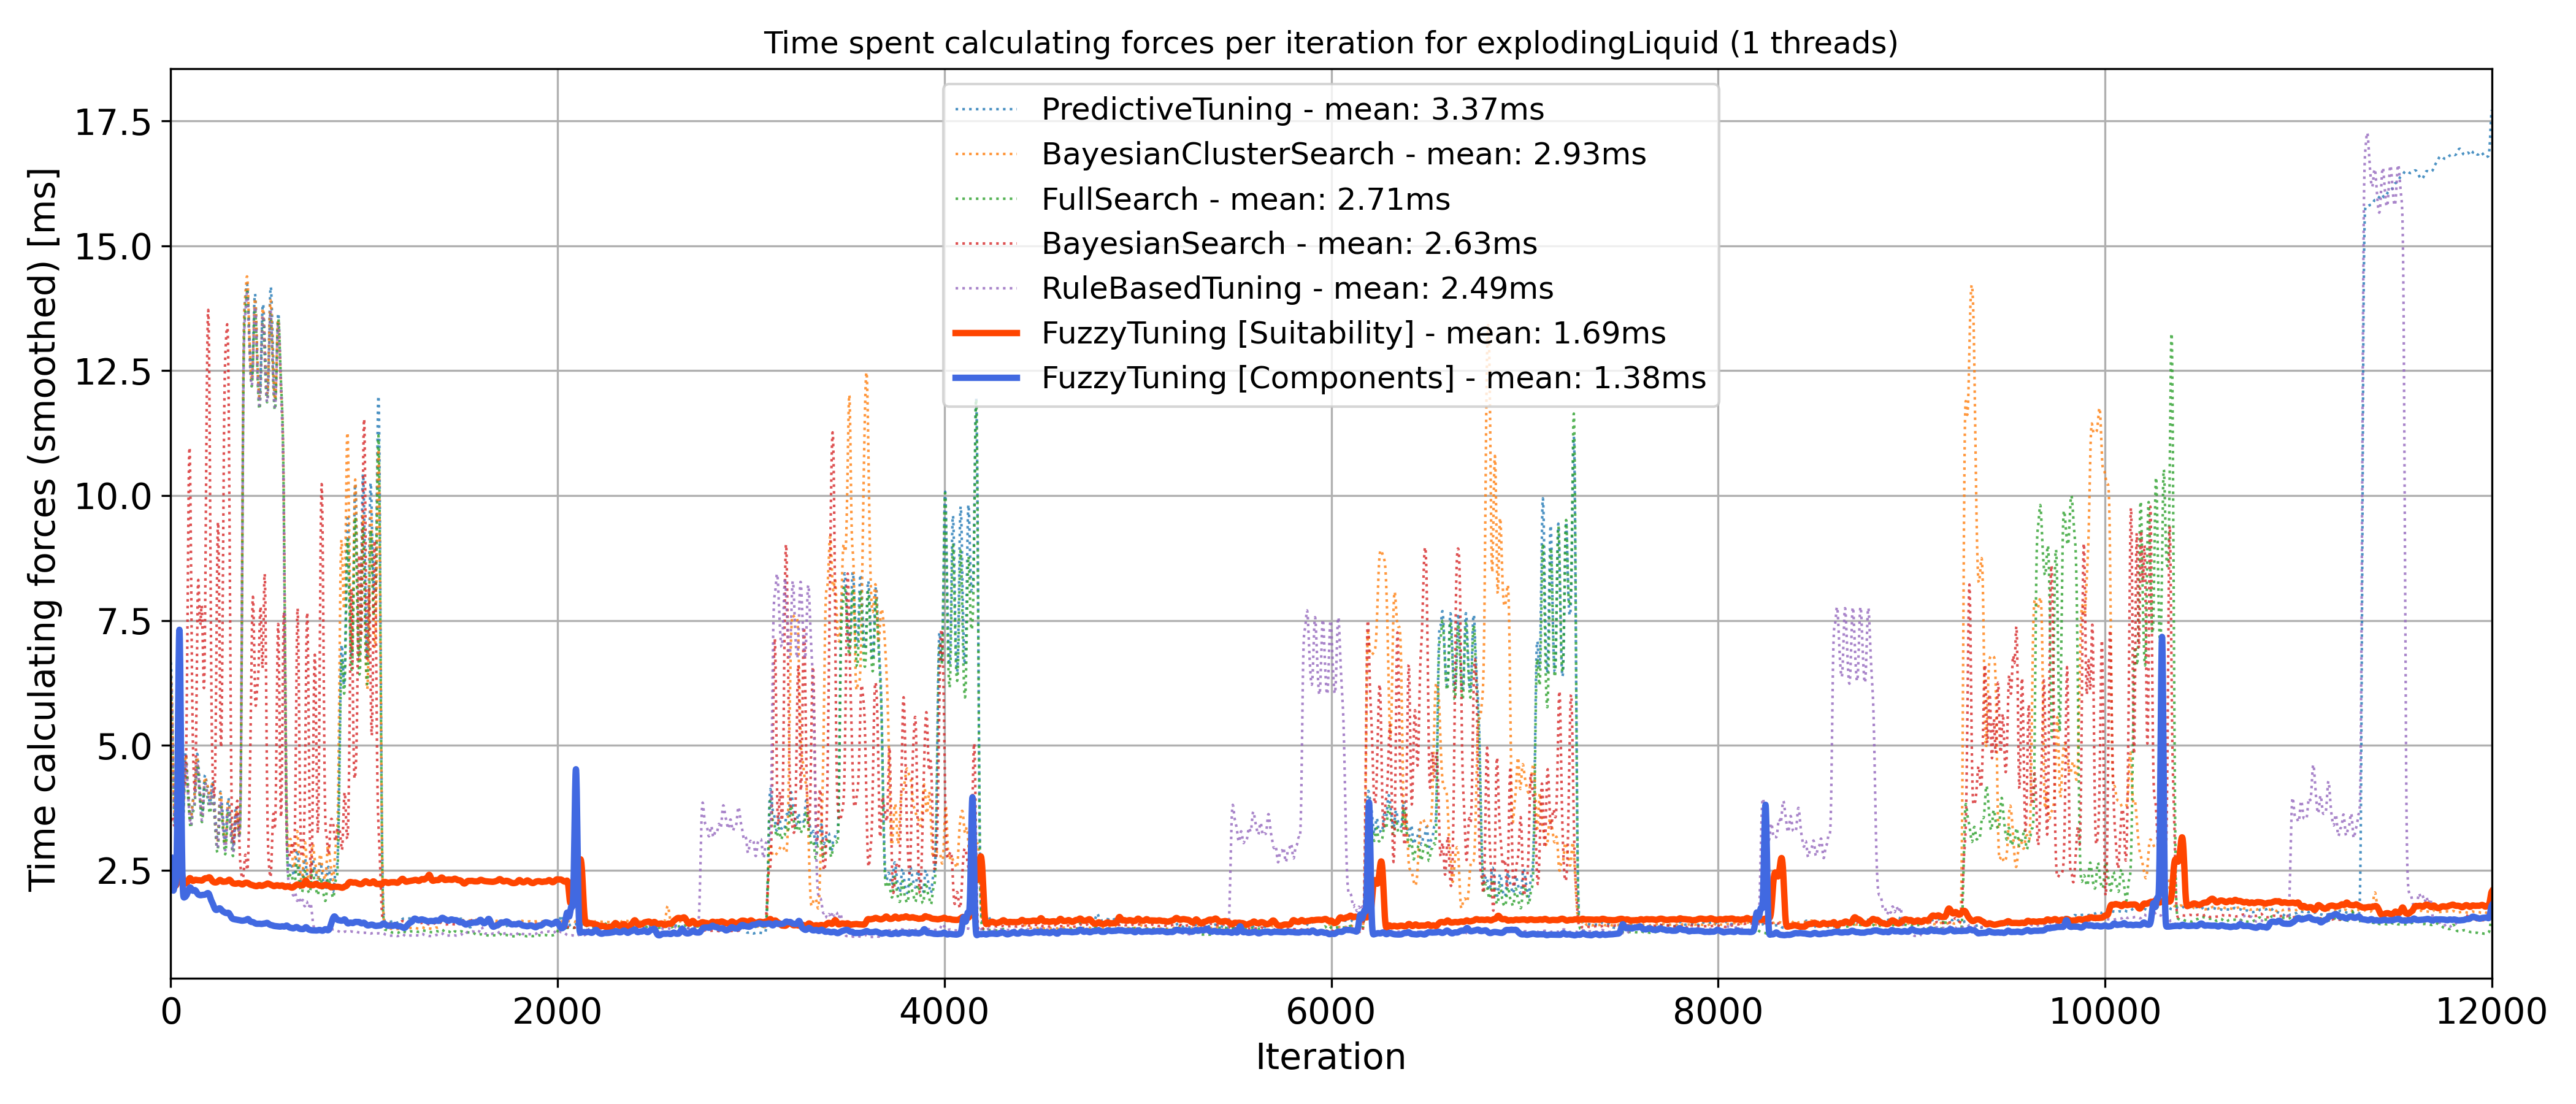
\includegraphics[width=\columnwidth,trim={0cm 0cm 0cm 0.9cm},clip]{figures/Benchmark/ExplodingLiquid/timing_explodingLiquid_1.png}
        \caption{}
        \label{fig:explodingTimings_1thread}
    \end{subfigure}


    \begin{subfigure}[c]{\textwidth}
        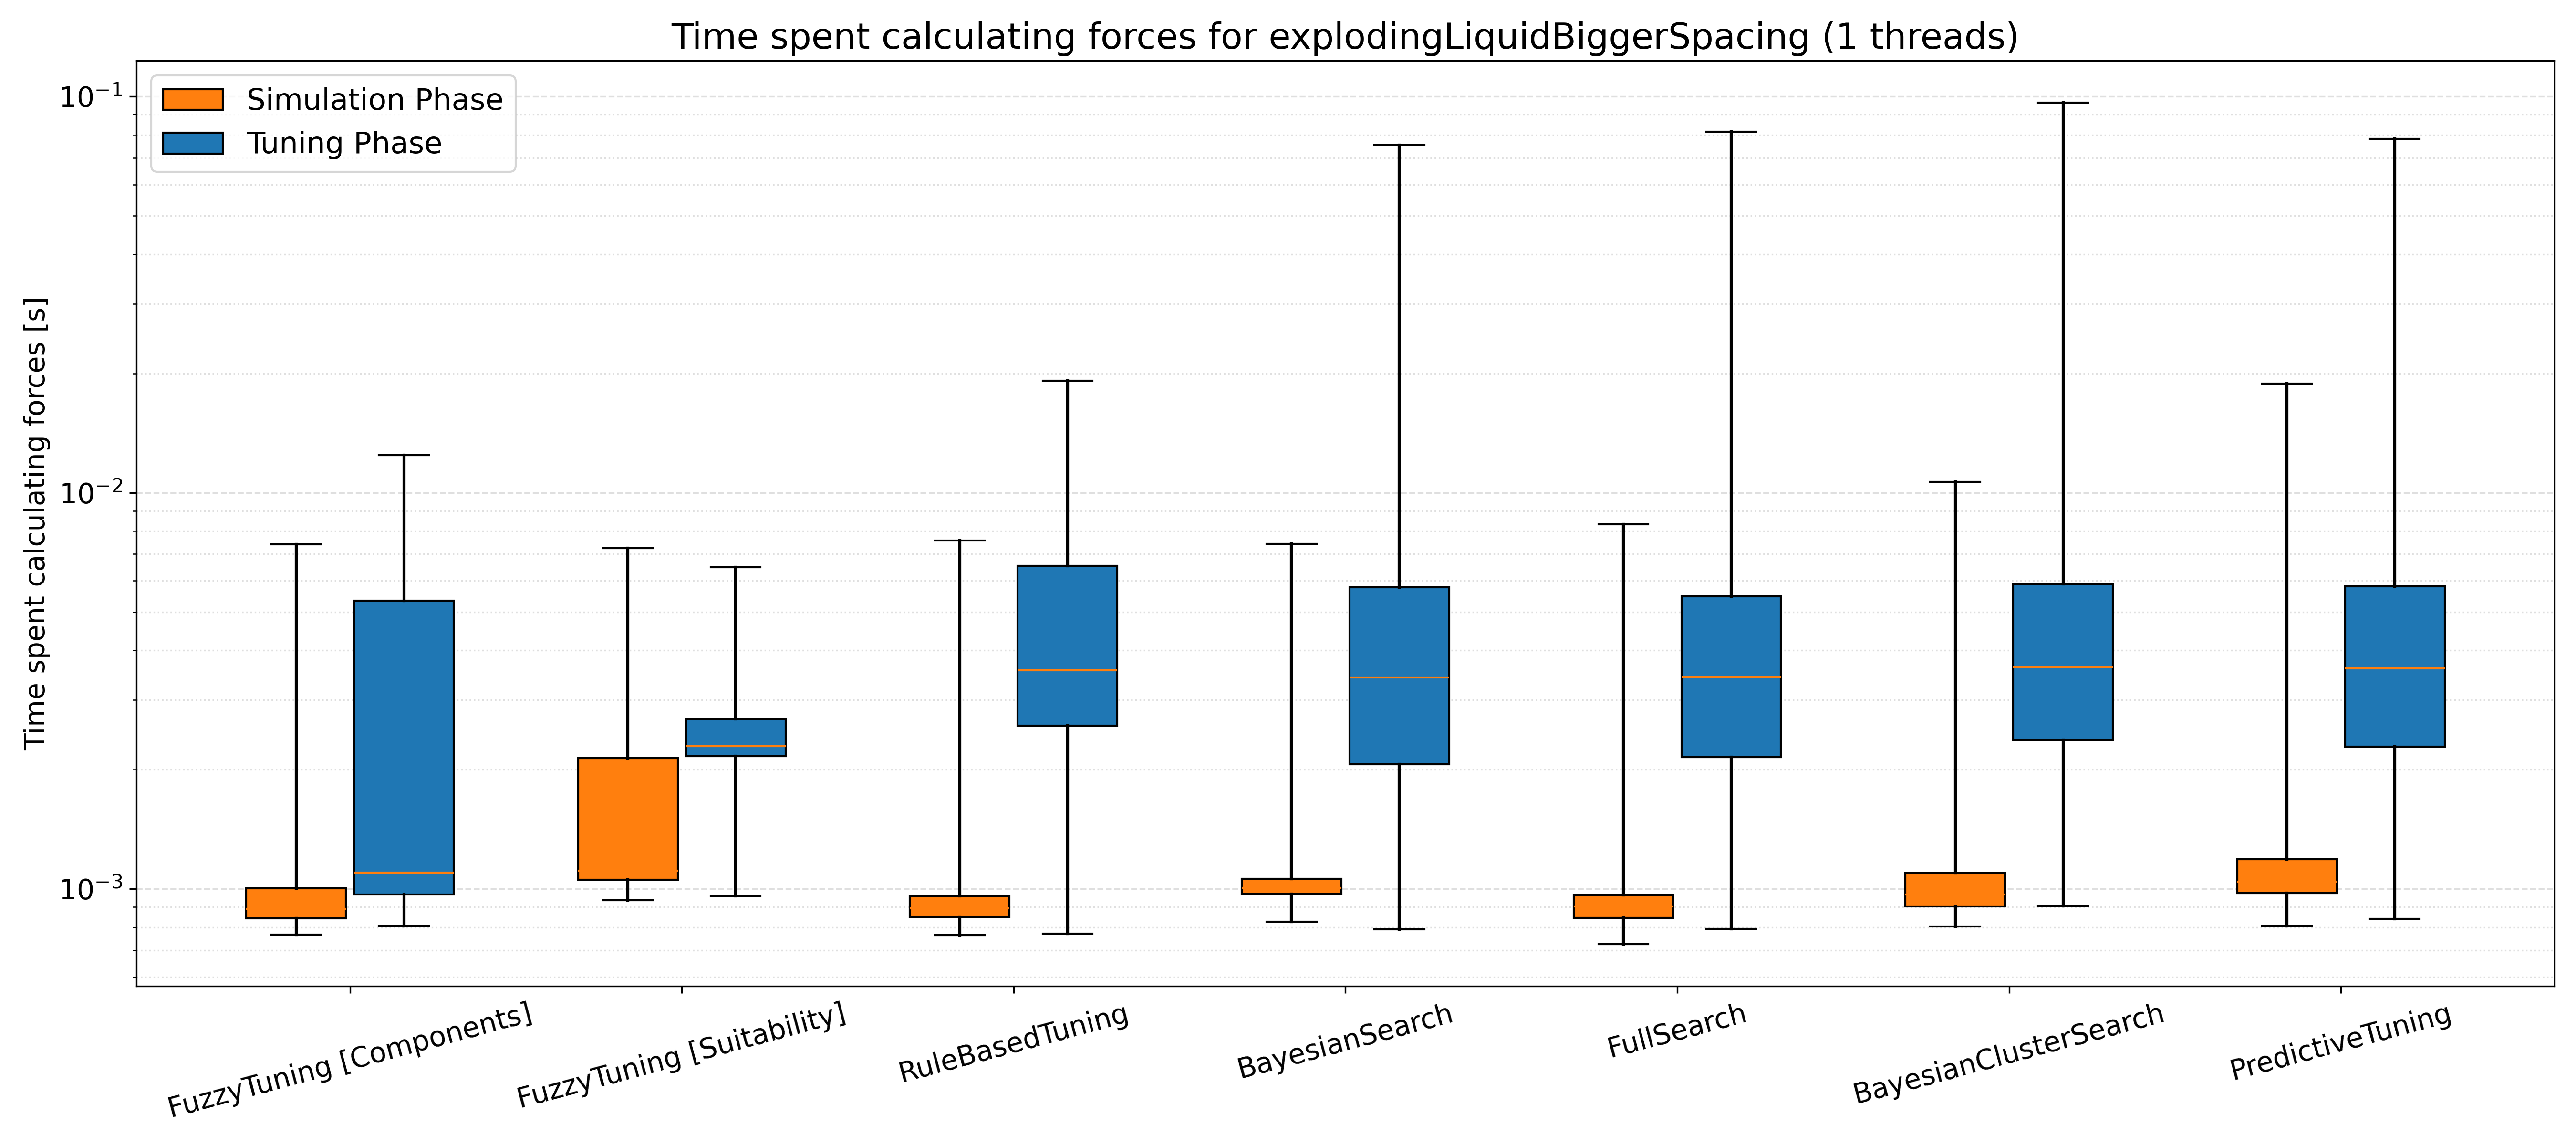
\includegraphics[width=\columnwidth,trim={0cm 0.5cm 0cm 1cm},clip]{figures/Benchmark/ExplodingLiquid/boxplot_explodingLiquid_1.png}
        \caption{}
        \label{fig:explodingLiquidBoxplot_1thread}
    \end{subfigure}

    \begin{subfigure}[b]{\textwidth}
        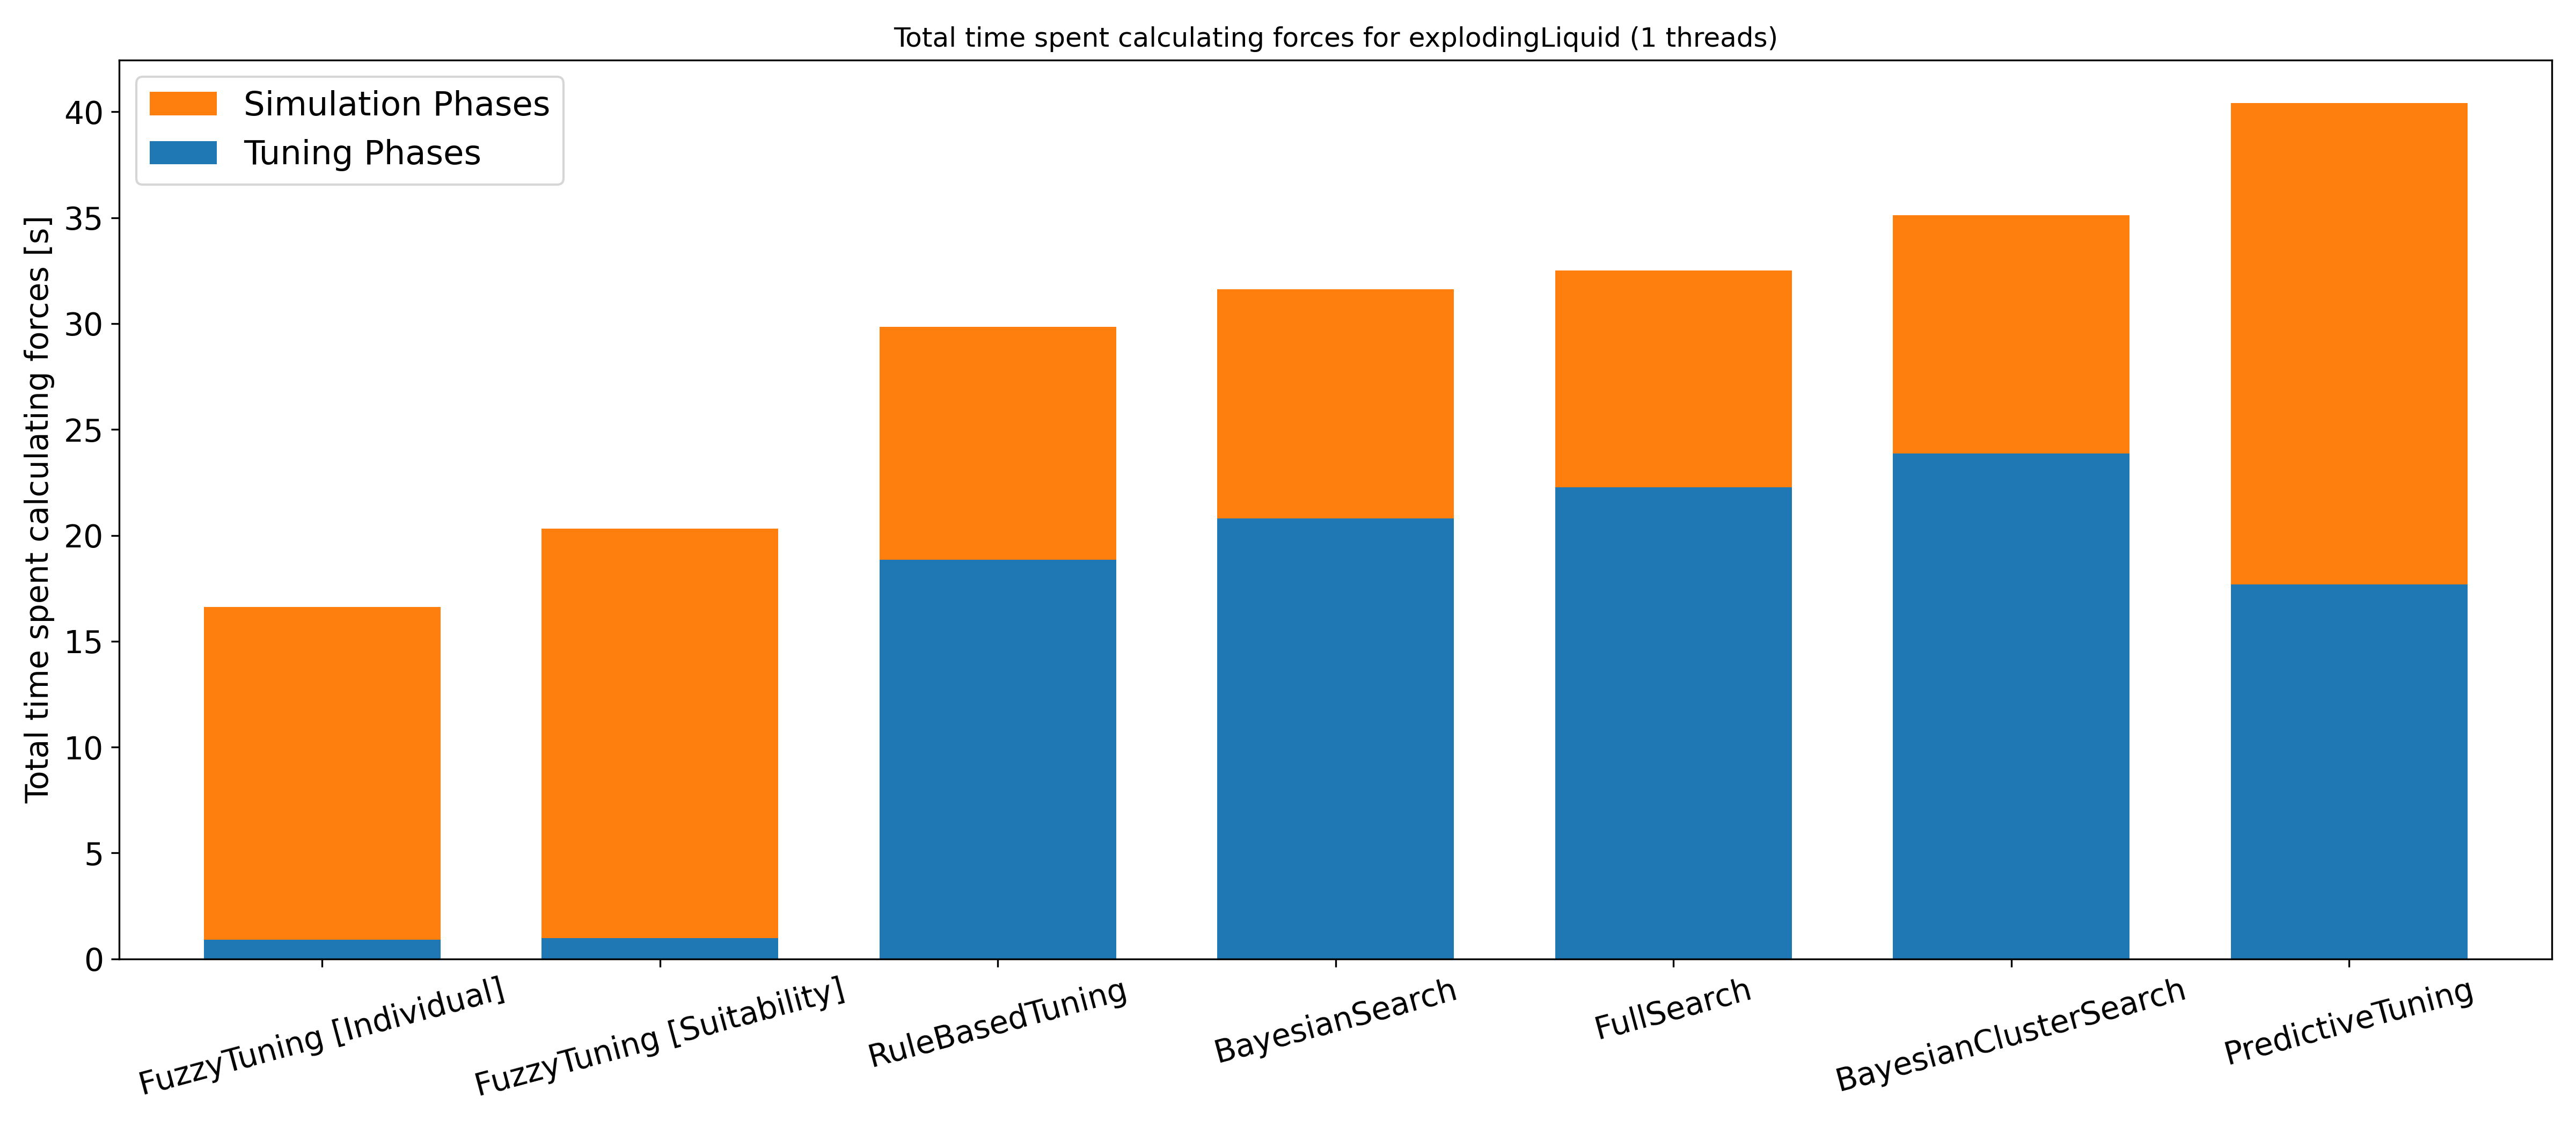
\includegraphics[width=\columnwidth,trim={0cm 0.5cm 0cm 0.9cm},clip]{figures/Benchmark/ExplodingLiquid/total_time_explodingLiquid_1.png}
        \caption{}
        \label{fig:explodingLiquidTotalTime_1thread}
    \end{subfigure}


    \caption[Exploding liquid benchmark with 1 thread]{Exploding liquid benchmark with 1 thread. (a) Time spent calculating forces for every iteration. (b) Boxplots of time spent calculating forces divided into tuning- and simulation phases. (c) Total time spent calculating forces for tuning- and simulation phases. The Suitability approach uses a non-optimal threshold of 10\% (see \autoref{sec:suitabilityThreshold}).}
    \label{fig:explodingLiquid_1thread}
\end{figure}

\begin{figure}[H]
    \centering

    \begin{subfigure}[c]{\textwidth}
        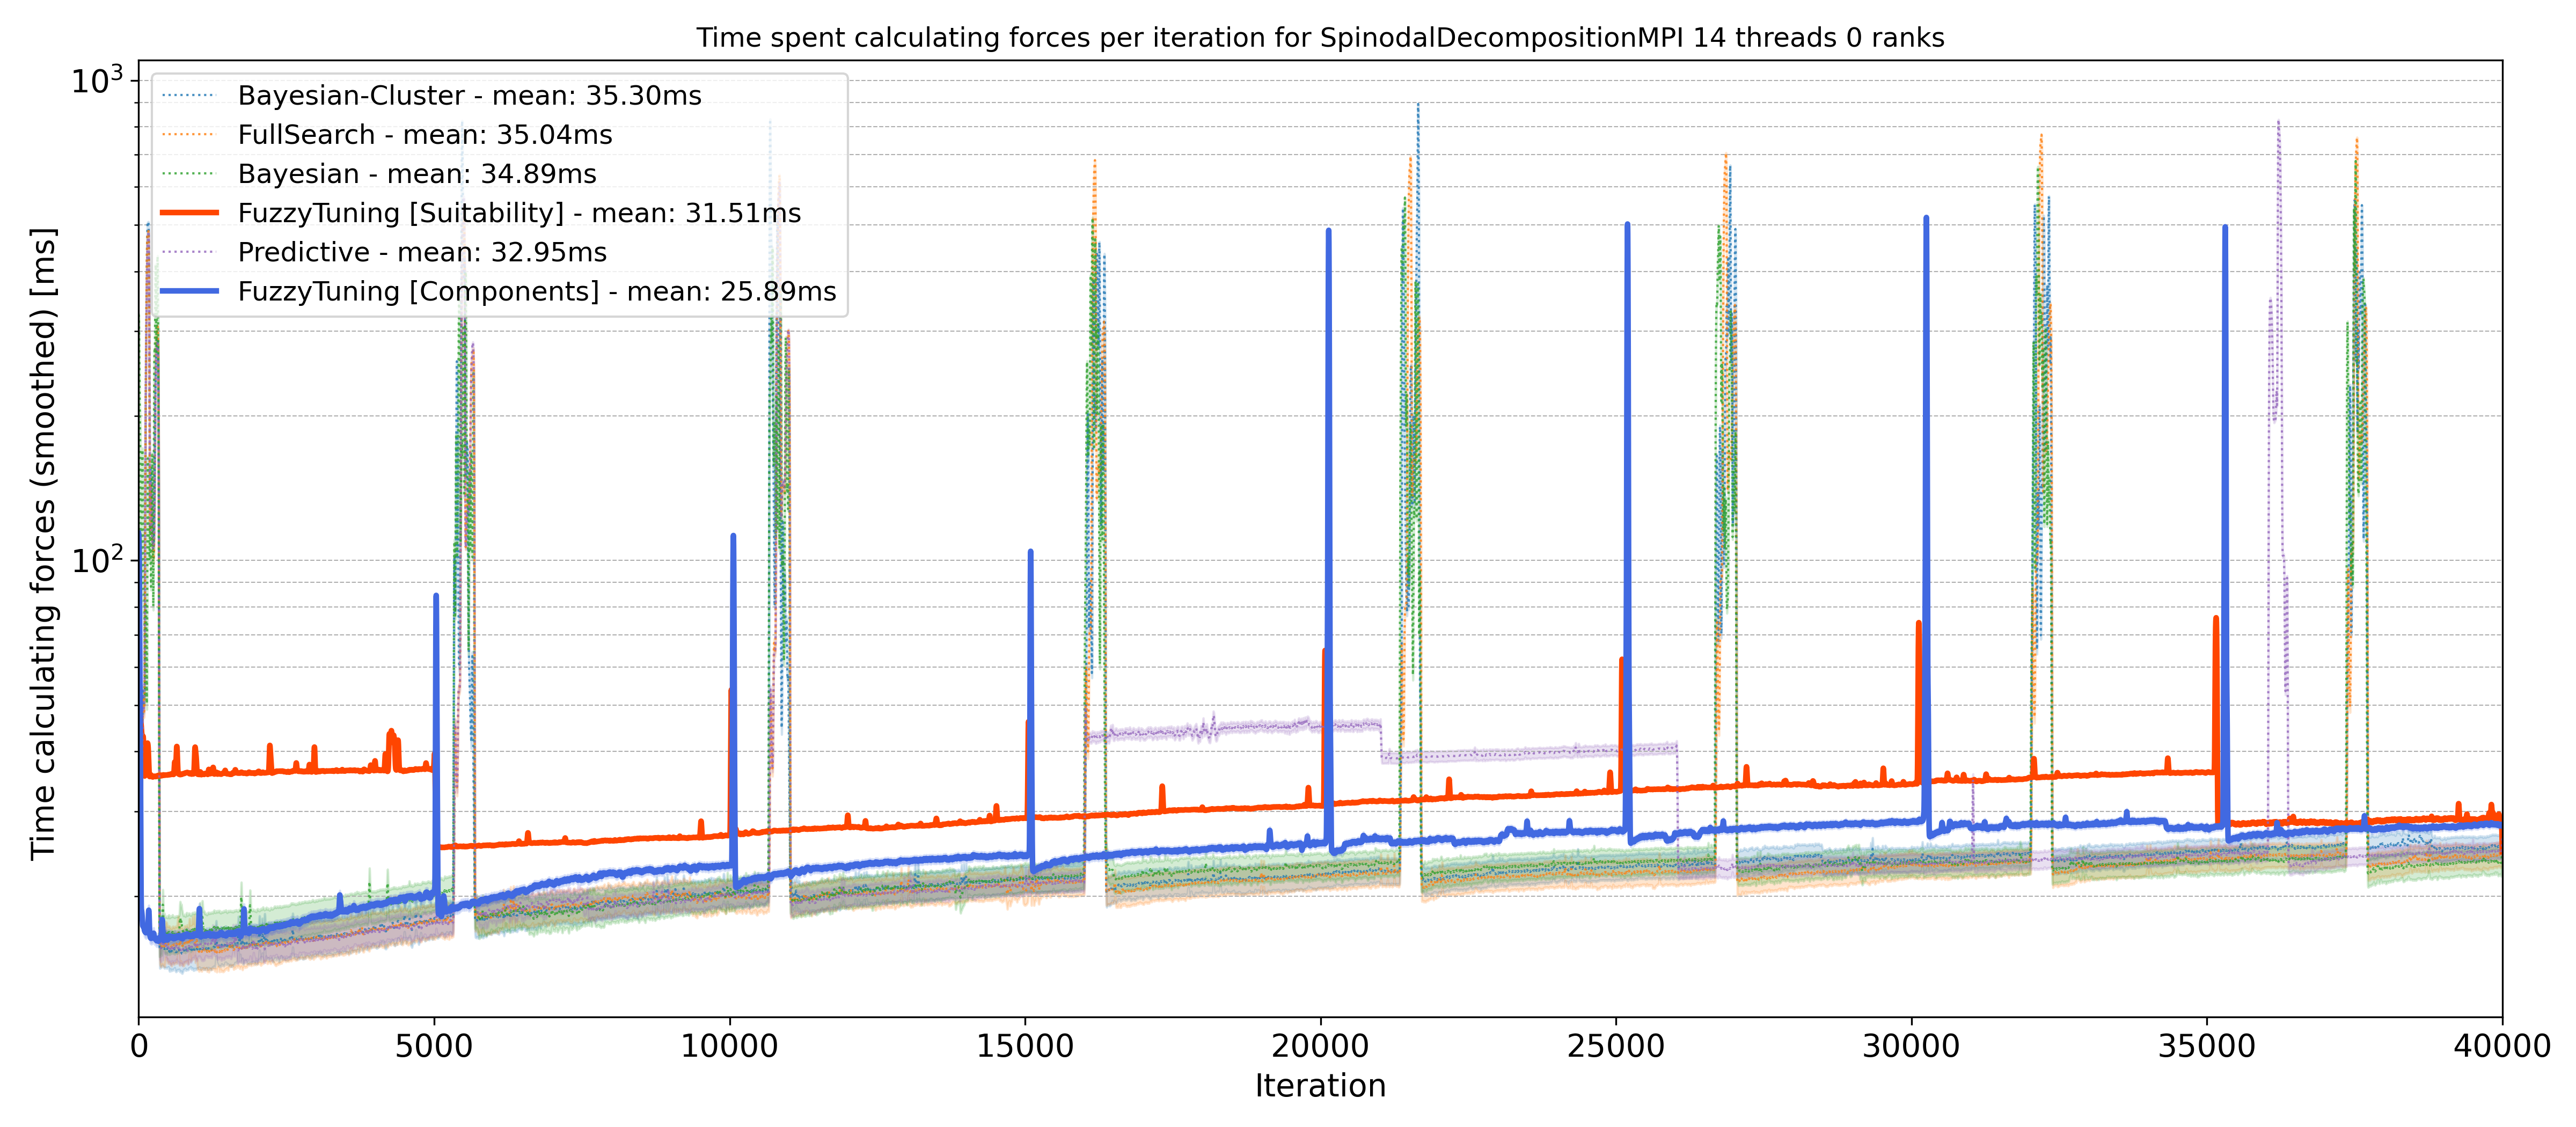
\includegraphics[width=\columnwidth,trim={0cm 0.2cm 0cm 0.9cm},clip]{figures/Benchmark/SpinodalDecompositionMPI/SpinodalDecompositionMPI_timings_SpinodalDecompositionMPI_14_0.png}
        \caption{}
        \label{fig:spinodalTimings_14thread}
    \end{subfigure}


    \begin{subfigure}[c]{\textwidth}
        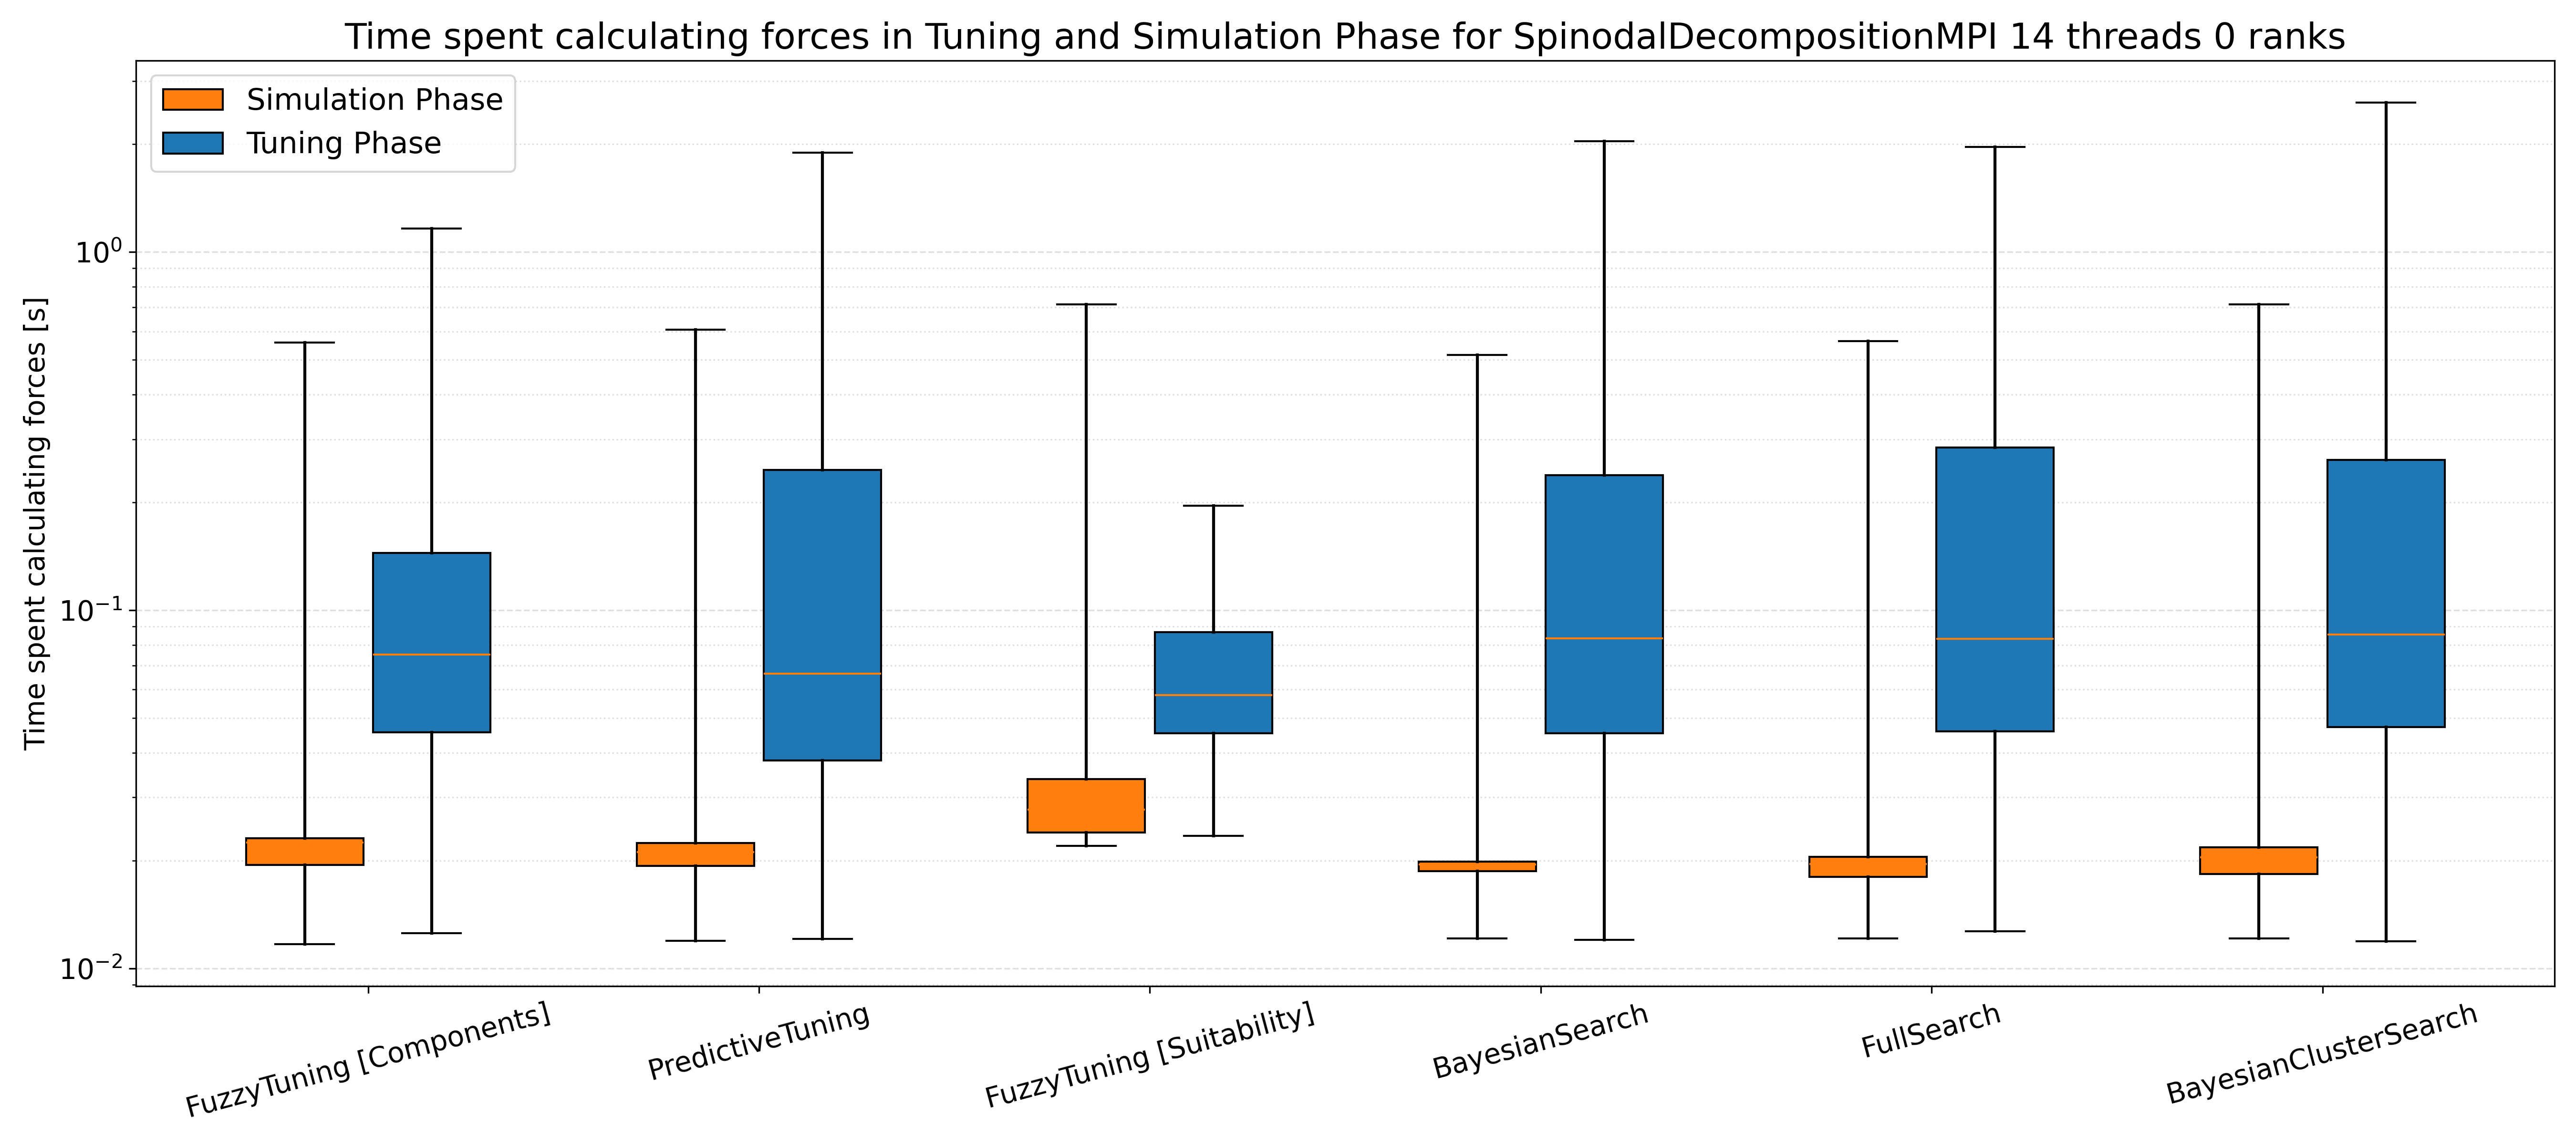
\includegraphics[width=\columnwidth,trim={0cm 0.5cm 0cm 1cm},clip]{figures/Benchmark/SpinodalDecompositionMPI/SpinodalDecompositionMPI_timings_boxplot_SpinodalDecompositionMPI_14_0.png}
        \caption{}
        \label{fig:spinodalBoxplot_14thread}
    \end{subfigure}

    \begin{subfigure}[b]{\textwidth}
        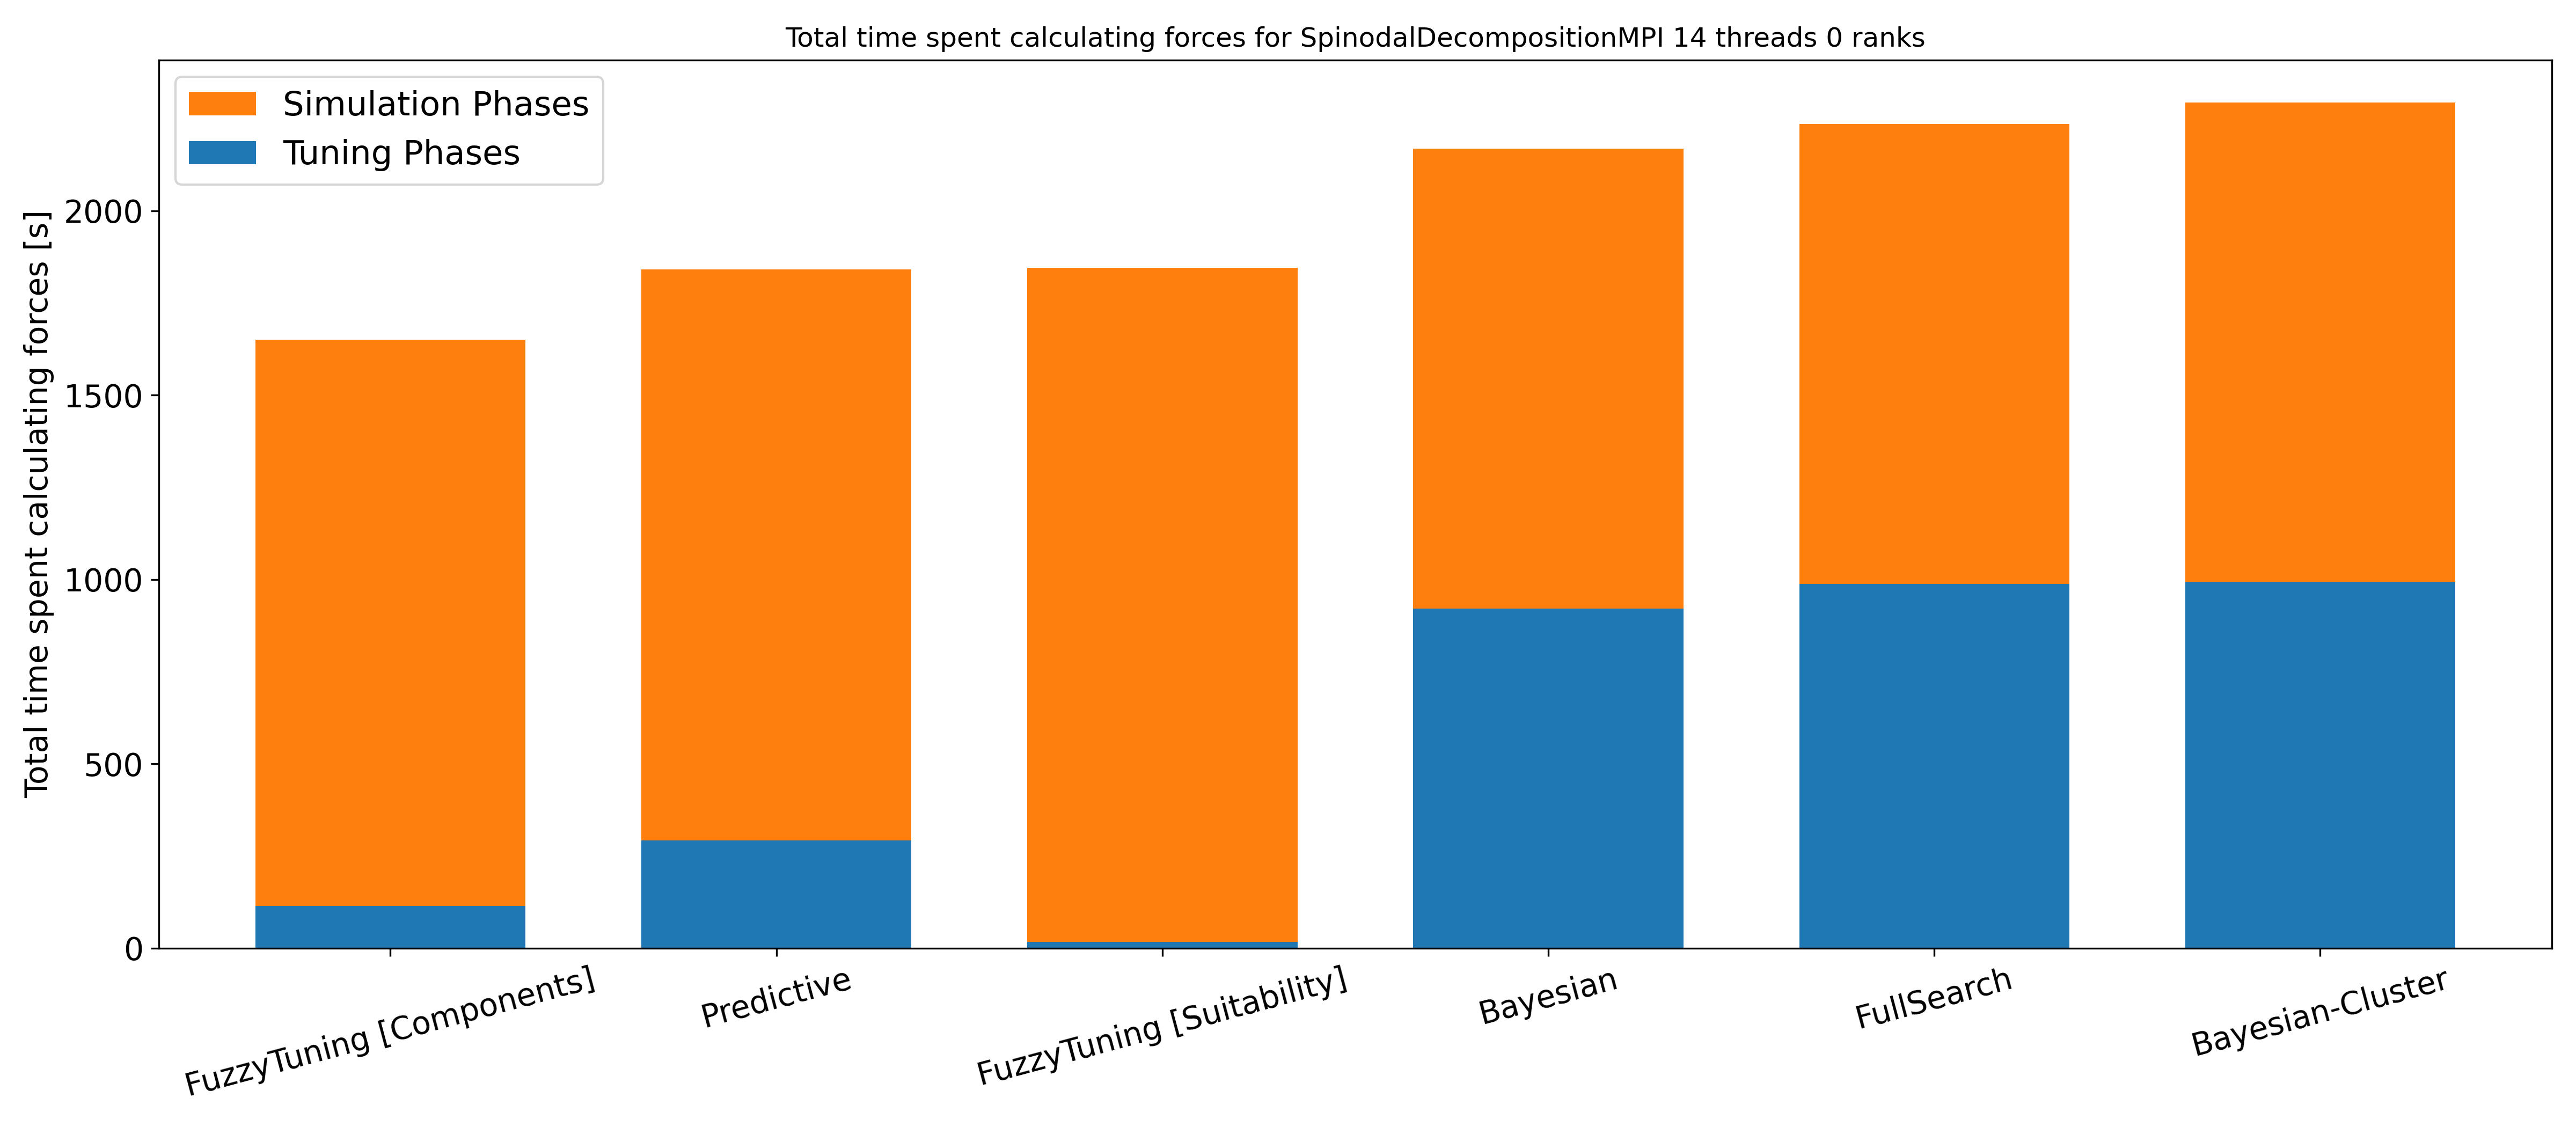
\includegraphics[width=\columnwidth,trim={0cm 0.5cm 0cm 0.9cm},clip]{figures/Benchmark/SpinodalDecompositionMPI/SpinodalDecompositionMPI_timings_total_SpinodalDecompositionMPI_14_0.png}
        \caption{}
        \label{fig:spinodalTotalTime_14thread}
    \end{subfigure}


    \caption[Spinodal decomposition benchmark MPI with 14 threads]{0th Rank of the Spinodal decomposition benchmark (Total: 4 MPI ranks, 14 threads each). (a) Time spent calculating forces for every iteration. (b) Boxplots of time spent calculating forces divided into tuning- and simulation phases. (c) Total time spent calculating forces for tuning- and simulation phases. The suitability approach uses a non-optimal threshold of 10\% (see \autoref{sec:suitabilityThreshold}).}
    \label{fig:spinodal_14thread}
\end{figure}



\section{Further Analysis}

\subsection{Quality of Predictions During Tuning Phases}

As described above, a tremendous slowdown of the classical tuning strategies is caused by very bad configurations that are sometimes encountered during the tuning phases. To further illustrate this, we will investigate the speedup density distribution of all configurations evaluated during the tuning phases of the different strategies. In particular, we will look at the Exploding Liquid and Spinodal Decomposition MPI scenarios described above, as they represent \emph{small} and \emph{large} scenarios, respectively.

The plots in \autoref{fig:tuningPhaseSpeedup} show these relative speedup distributions. All classical tuning strategies tend to encounter configurations with extremely low speedups during the tuning phases. In the exploding-liquid benchmark, some bad configurations are $\sim10$ times slower than the winning configurations, while we observe iterations $\sim100$ times slower in the Spinodal Decomposition MPI scenario.

The fuzzy tuning strategies, especially the suitability approach, predict much better configurations during the tuning phases. Combined with the relatively small number of configurations evaluated during the tuning phases, this leads to very short tuning phases for this strategy while still finding close to optimal configurations, as shown in the previous sections. However, the relatively small number of evaluated configurations of the suitability approach is also a disadvantage, as it causes the strategy to sometimes miss the optimal configuration.
The component tuning approach evaluates more, possibly suboptimal, configurations during the tuning phases, which causes bigger spikes in the time spent calculating forces, which can be seen in \autoref{fig:explodingTimings_1thread} and \autoref{fig:spinodalTimings_14thread}. Those spikes are relatively short and rare and do not significantly impact the strategy's overall performance. This causes the component tuning approach to perform better than the suitability approach in most scenarios.
In \autoref{sec:suitabilityThreshold}, we will investigate the suitability threshold and its impact on the performance of the suitability approach.

\smallskip

A possible improvement to AutoPas would be to automatically detect such bad configurations while evaluating them and discard them early if they are significantly worse than the current best configuration. Such an improvement could drastically benefit every tuning strategy by significantly reducing the time spent in the tuning phases while still finding the same optimal configuration.


\newpage

\begin{figure}[H]
    \centering

    \begin{subfigure}[c]{\textwidth}
        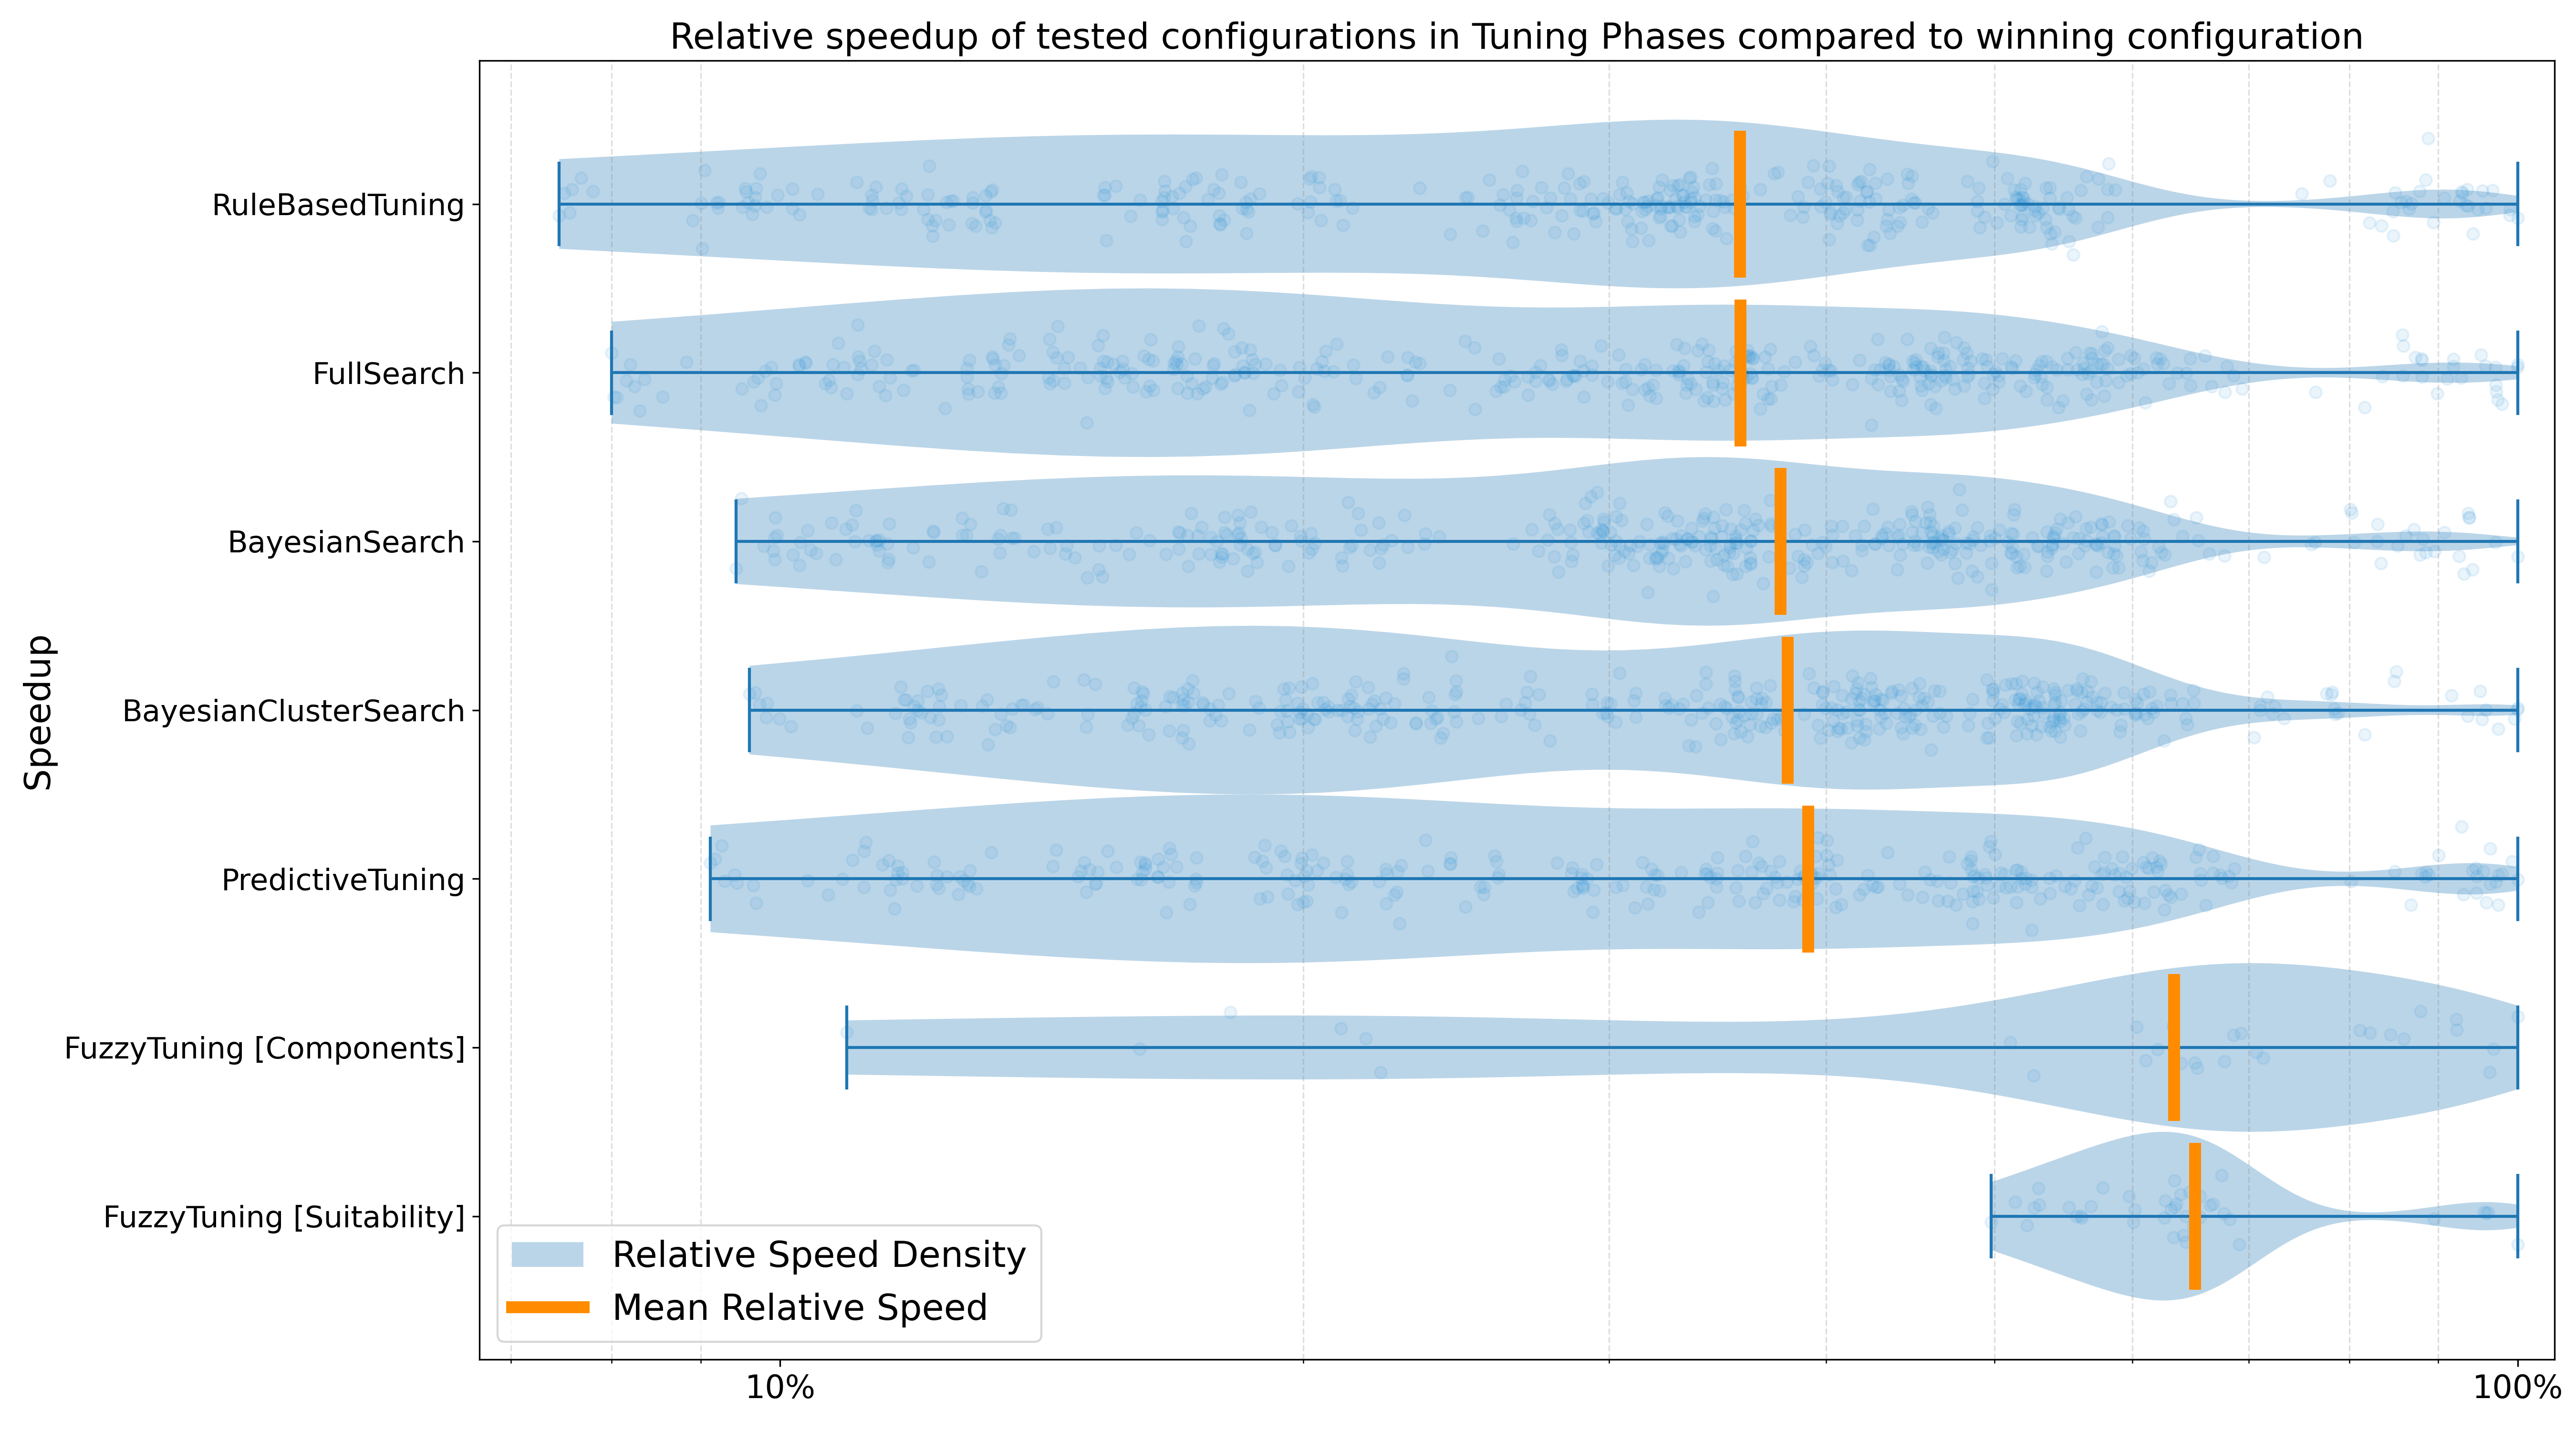
\includegraphics[width=\columnwidth,trim={1cm 0 0cm 1cm},clip]{figures/Benchmark/Observations/tuning_phase_speedup_explodingLiquid_1_zoomed.png}
        \caption{Exploding Liquid scenario with one thread.}
        \label{fig:explodingLiquidSpeedupDensity}
    \end{subfigure}


    \begin{subfigure}[c]{\textwidth}
        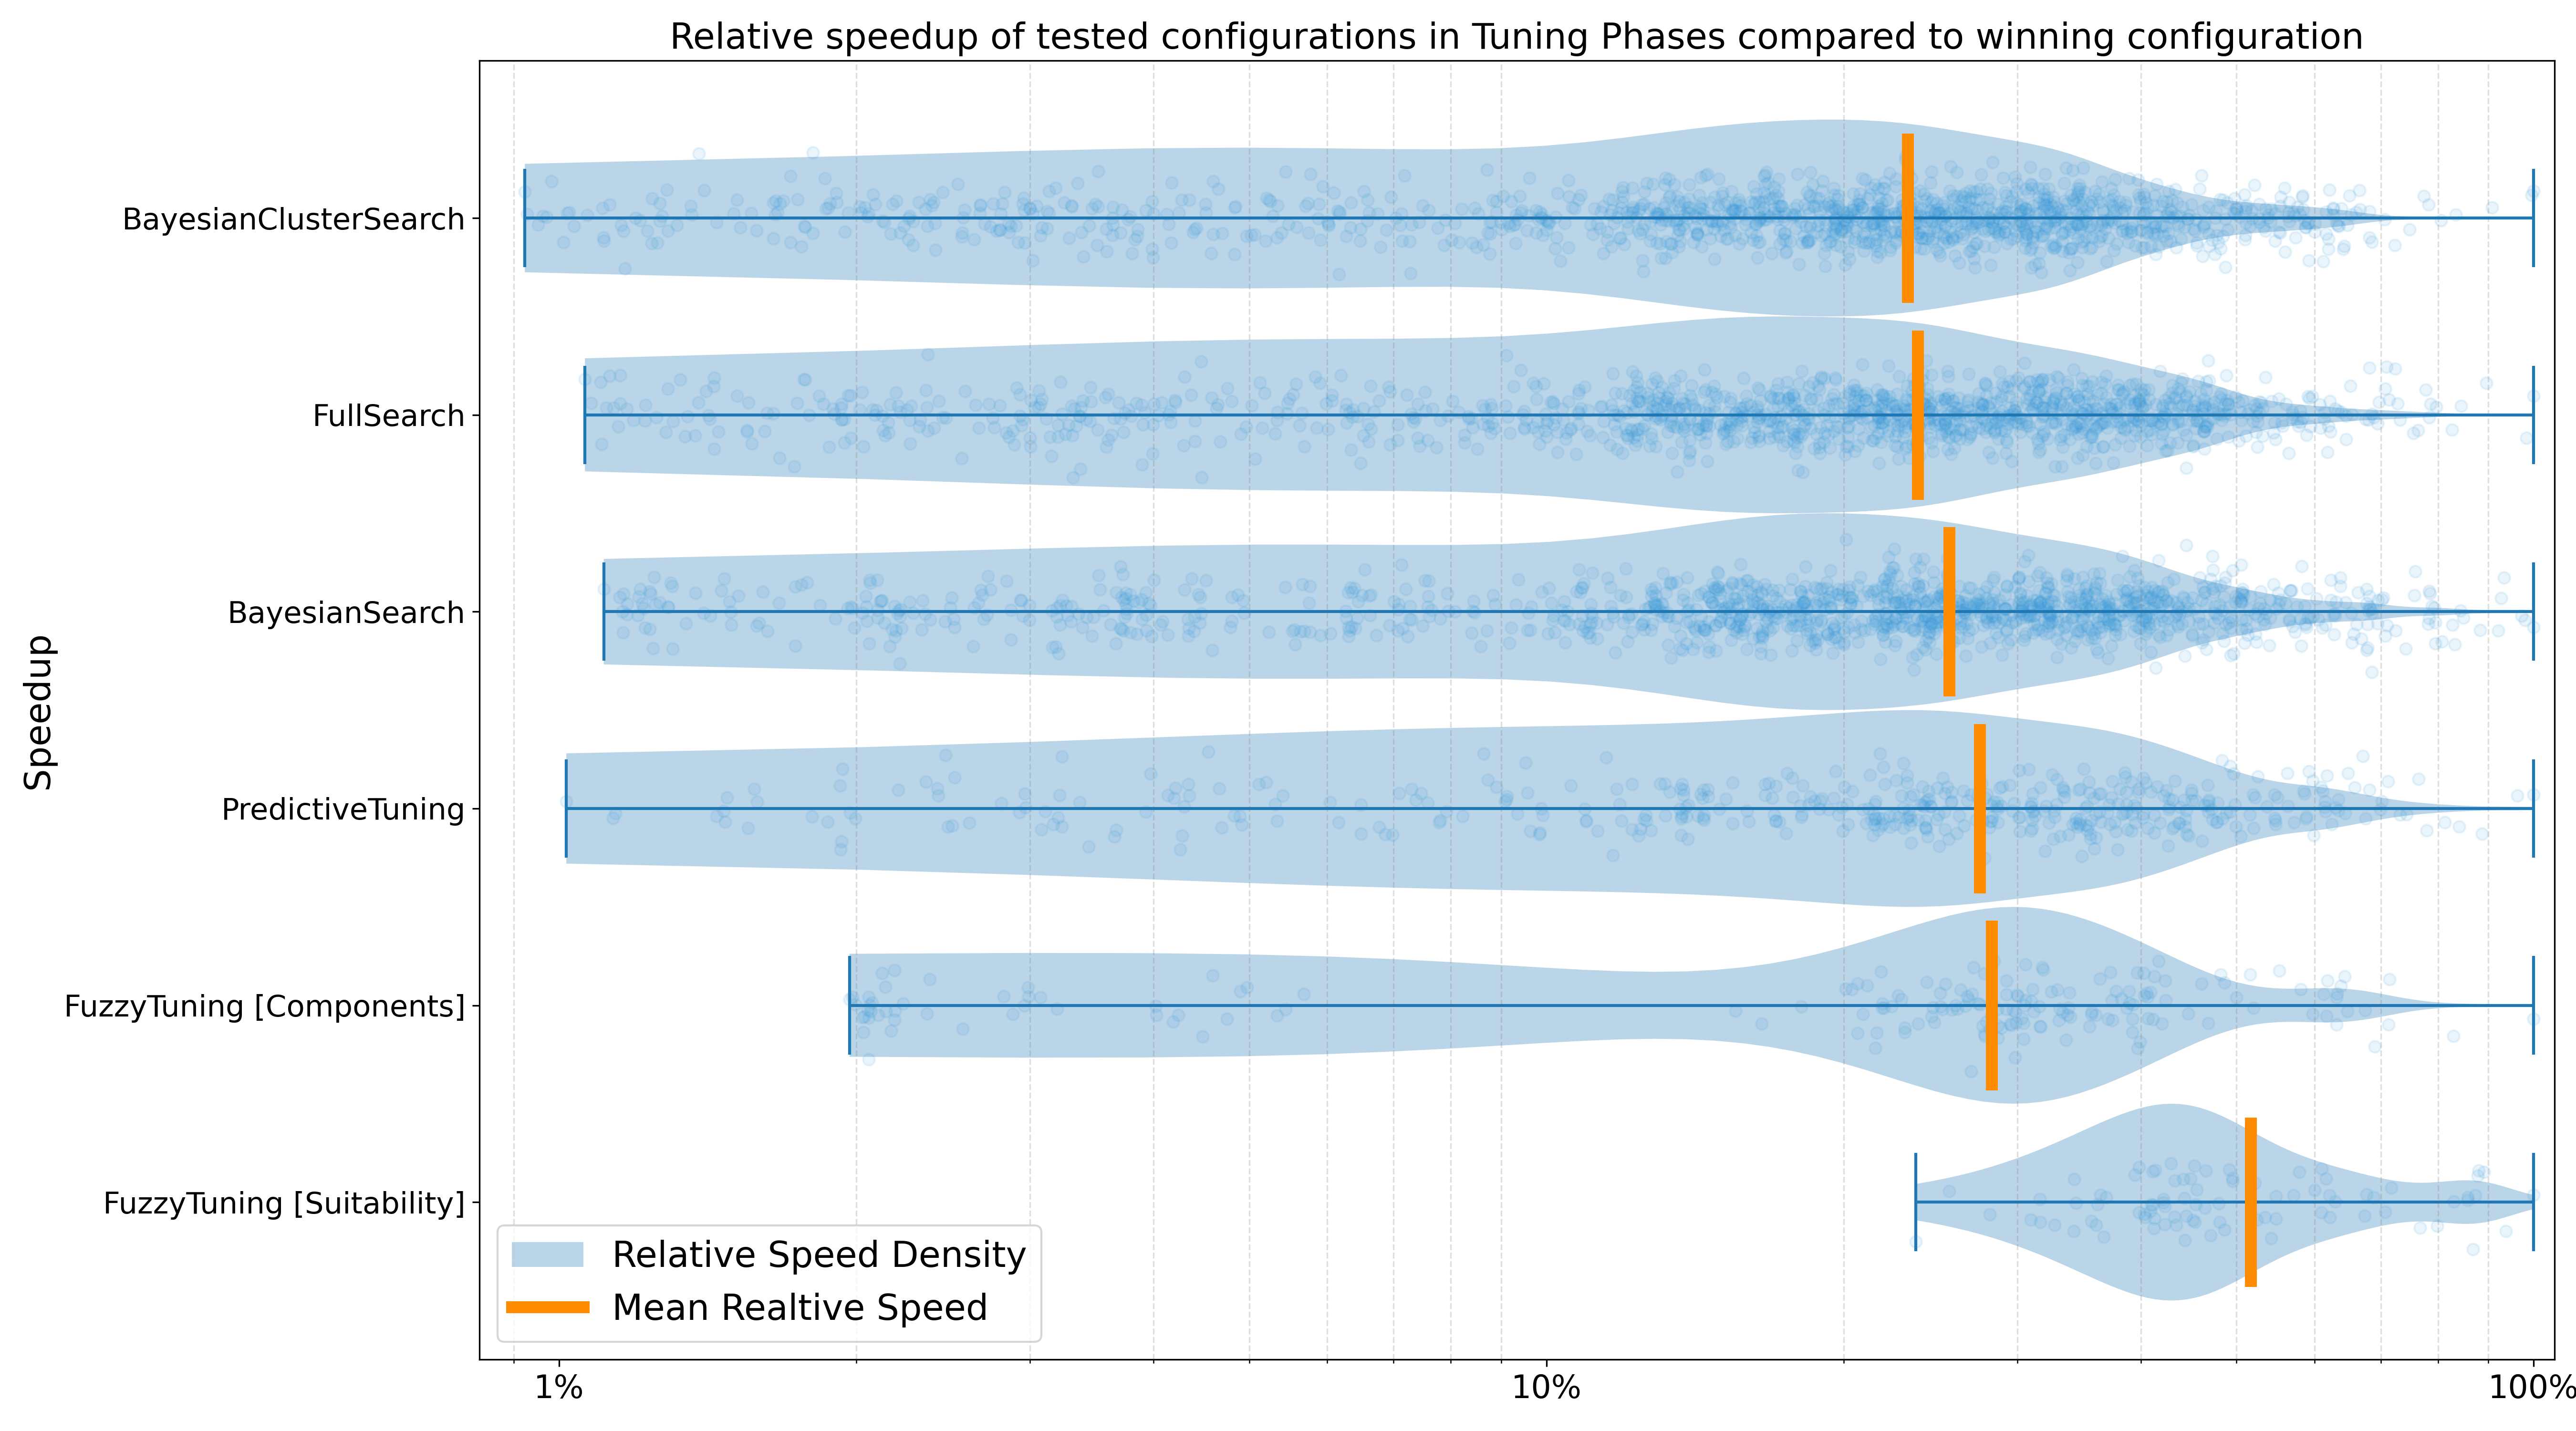
\includegraphics[width=\columnwidth,trim={1cm 0 0cm 1cm},clip]{figures/Benchmark/Observations/tuning_phase_speedup_SpinodalDecompositionMPI_14_0.png}
        \caption{Rank 0 of the Spinodal Decomposition MPI scenario with 14 threads.}
        \label{fig:spinodalSpeedupDensity}
    \end{subfigure}


    \caption[Quality of predictions during tuning phases]{The plot shows the speedup density distribution of all configurations evaluated during the tuning phases of both the Exploding Liquid and Spinodal Decomposition MPI scenarios calculated from the smoothed timings (see \autoref*{des:tuningdatafields}). The fuzzy tuning strategies generally encounter better configurations during the tuning phases, which improves their total performance.}
    \label{fig:tuningPhaseSpeedup}
\end{figure}

\subsection{Suitability Threshold}
\label{sec:suitabilityThreshold}

In previous measurements, the Component tuning approach performed better than the Suitability tuning approach, mainly due to the suitability approach not finding the optimal configuration during the tuning phases (see \autoref{fig:explodingLiquid_1thread} and \autoref{fig:spinodal_14thread}).
Currently, the rule file for the suitability approach specifies that only the top 10\% of configurations with the highest suitability should be selected, which may be too low, as this results in extremely few configurations being selected for the tuning phases, resulting in a high chance of not finding the optimal configuration.

To investigate this further, we ran the Exploding Liquid benchmark with different suitability thresholds, as shown in \autoref{fig:suitabilityThreshold}. Very low thresholds perform poorly, as they select too few configurations for the tuning phases, resulting in a high chance of not finding the optimal configuration. Very high thresholds also perform poorly, as high suitability values cause the strategy to behave like FullSeach as it selects nearly all configurations for the tuning phases. The optimal suitability threshold for this scenario is between 20\% and 40\%, which guarantees that the best configuration is selected for the tuning phases while still keeping the number of configurations low.


Therefore, we recommend using a slightly higher suitability threshold for the suitability approach between 20\% and 40\% to improve the chances of finding the optimal configuration during the tuning phases without causing too much overhead by evaluating too many configurations.


\begin{figure}[H]
    \centering
    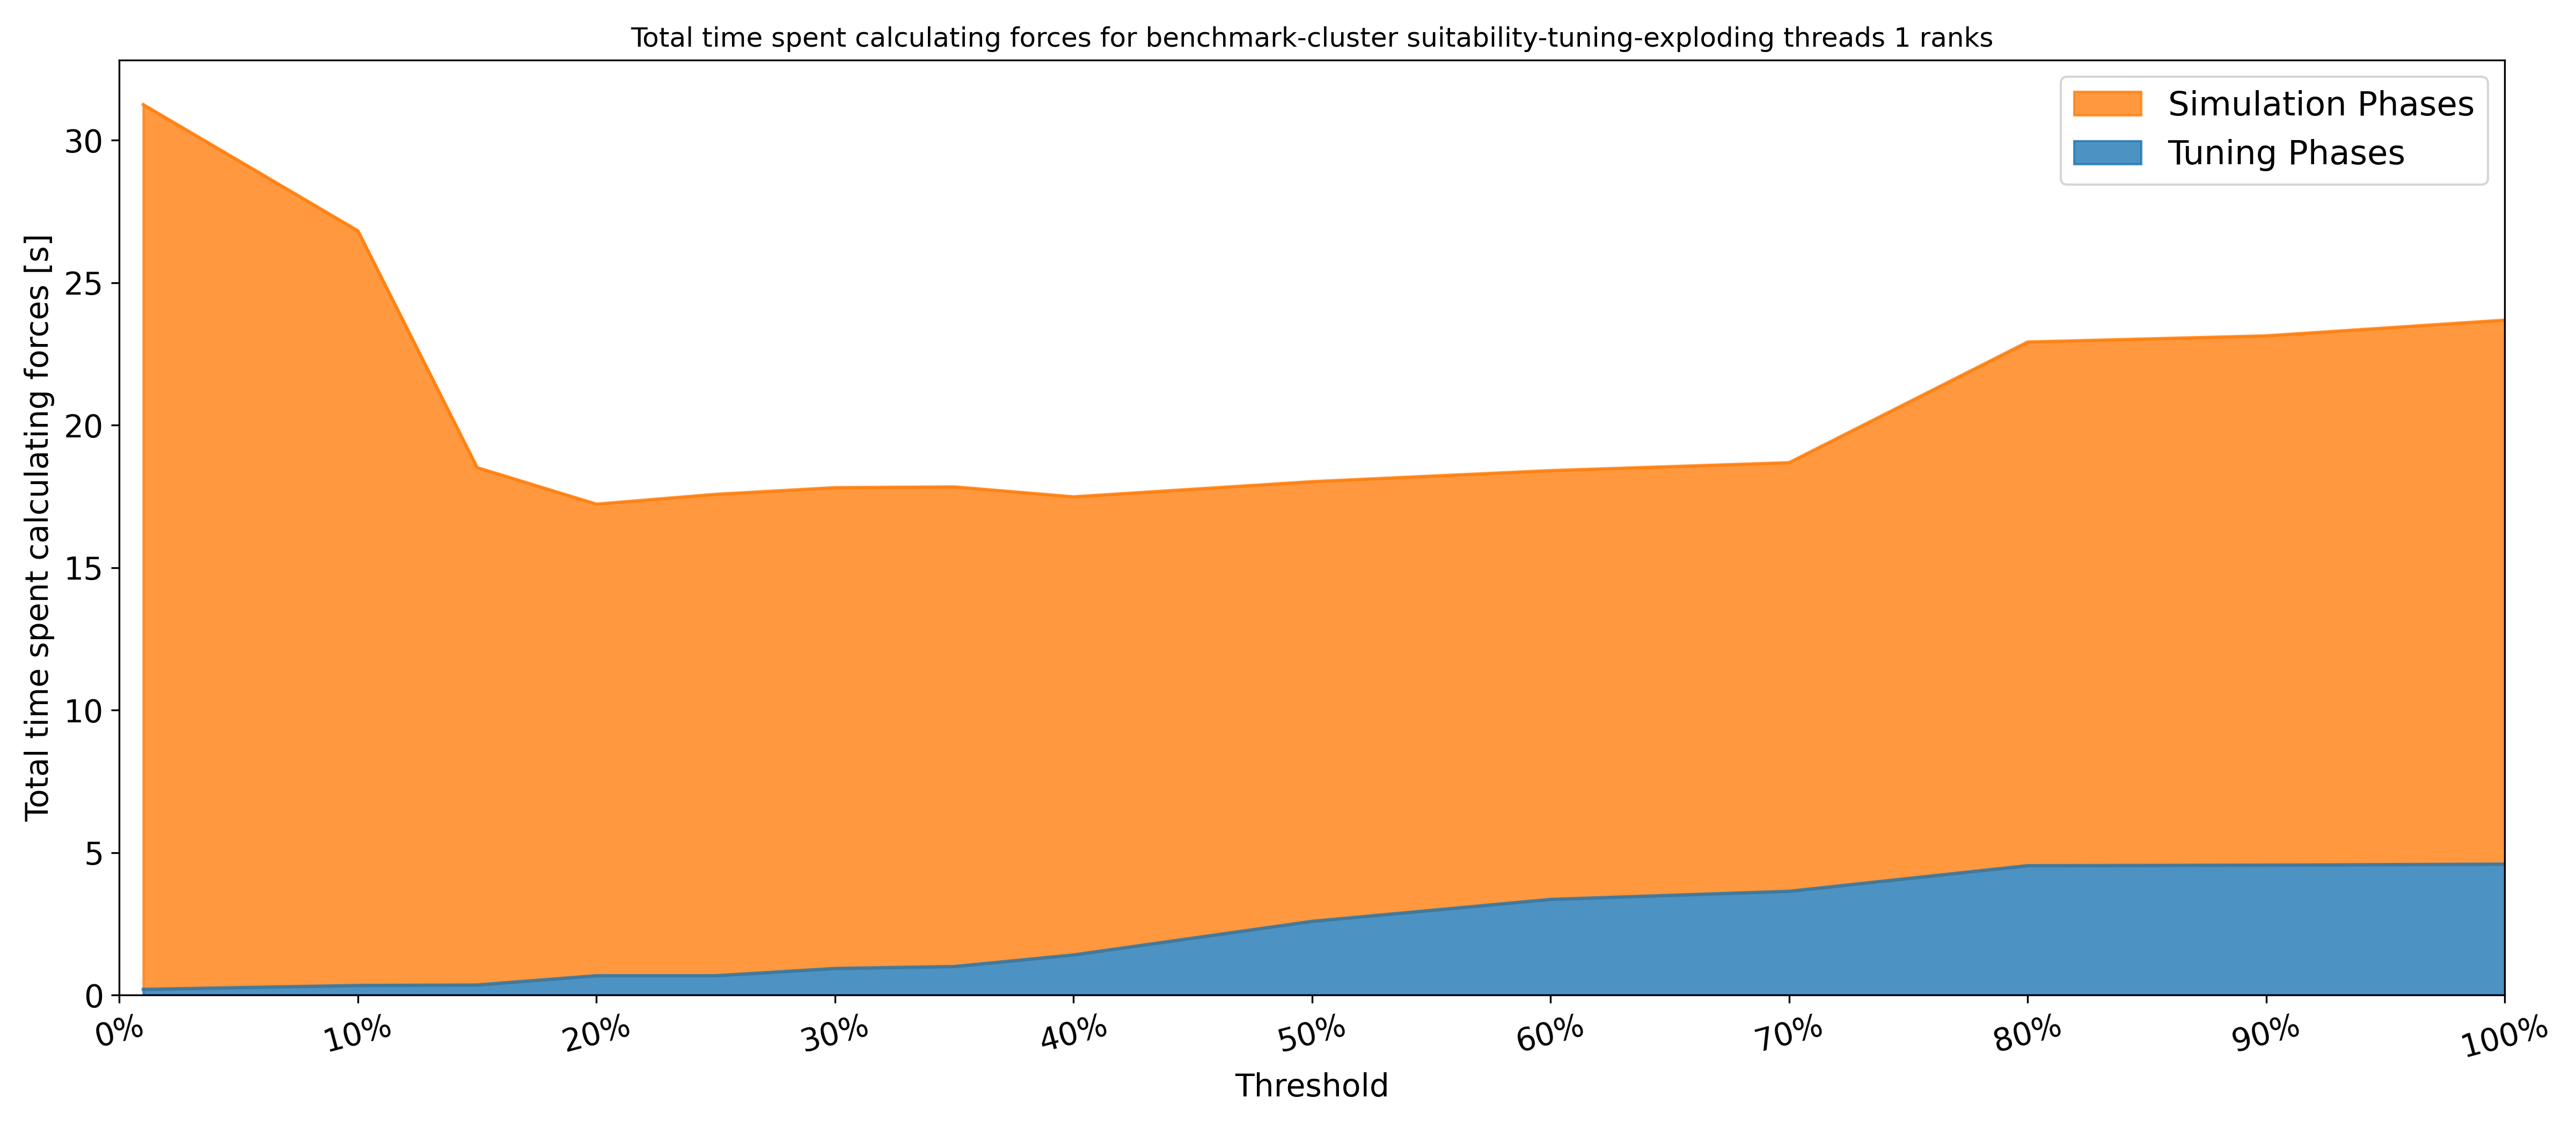
\includegraphics[width=\columnwidth]{figures/Benchmark/SuitabilitySearch/SuitabilityExploding_timings_threshold_benchmark-cluster_suitability-tuning-exploding_1.png}
    \caption[Exploding liquid benchmark with different suitability thresholds]{Exploding liquid benchmark with different suitability thresholds. The fastest runtimes are achieved with a threshold between 20\% and 40\%.}
    \label{fig:suitabilityThreshold}
\end{figure}

\newpage

\subsection{Robustness of the Fuzzy Tuning Strategies}

Previous measurements carried out in \autoref{sec:explodingLiquidBenchmark} directly included the Exploding Liquid benchmark in the training data, which could have biased the results in favor of the fuzzy tuning strategies. To investigate the robustness of the fuzzy tuning strategies, we reran the rule extraction process without the Exploding Liquid scenario in the training data and performed the Exploding Liquid benchmark again.

The results in \autoref{fig:explodingTimings_1thread_noTrainingData} show that the fuzzy tuning strategies still perform remarkably well, even without ever encountering the Exploding Liquid scenario during the rule extraction process. Therefore, we conclude that the rule extraction process is robust and can be generalized to similar scenarios, even if they were not included in the training data.

\begin{figure}[H]
    \centering

    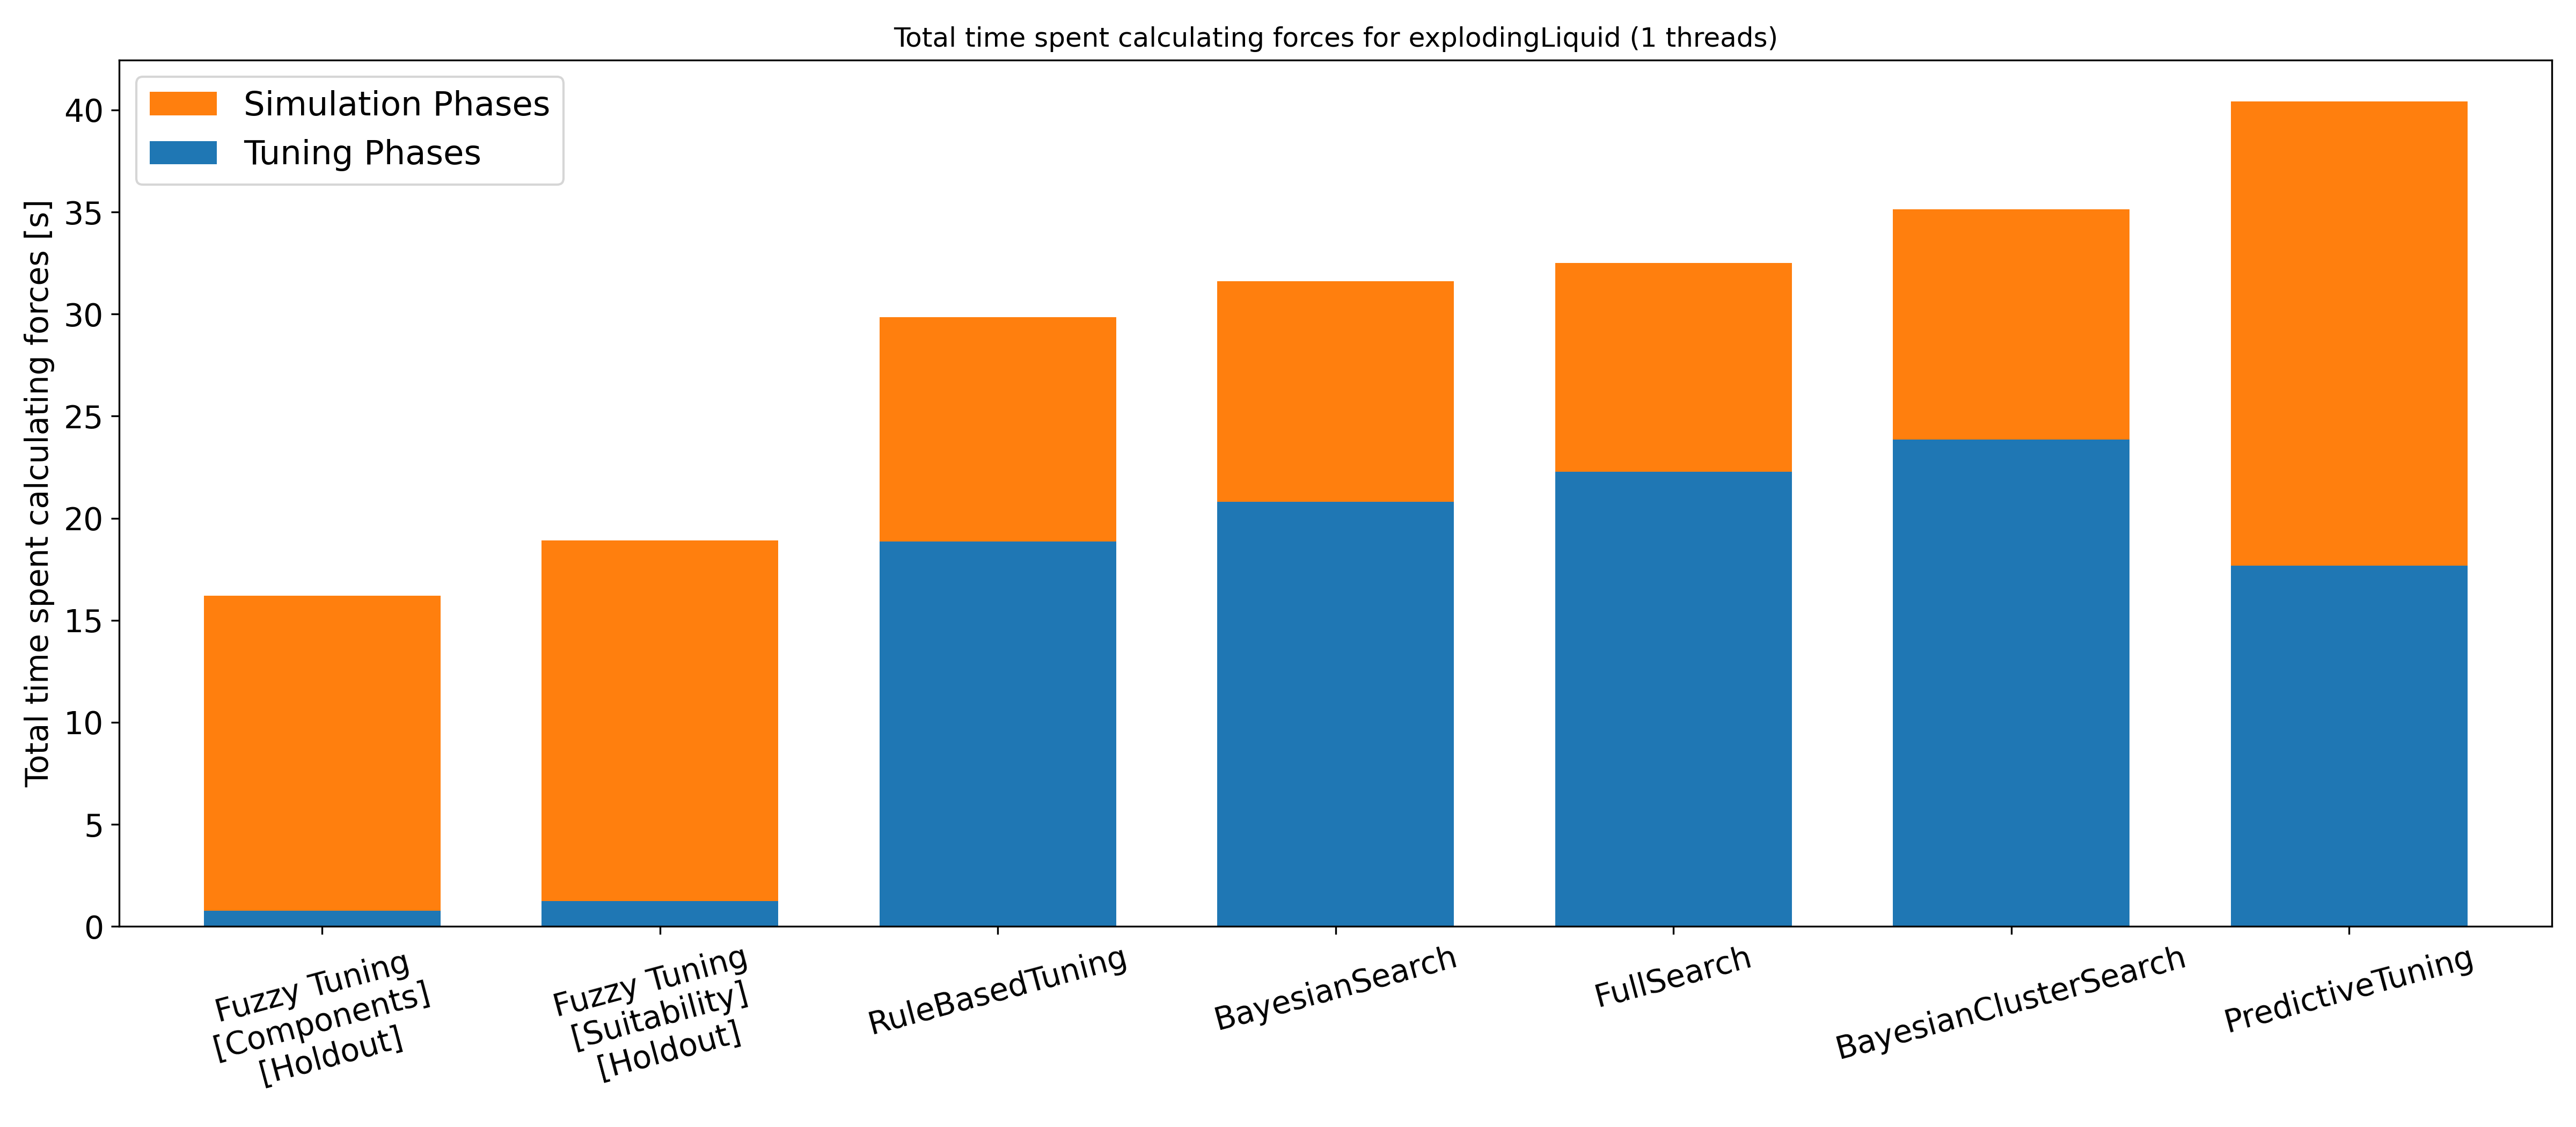
\includegraphics[width=\columnwidth,trim={0cm 0 0cm 0.9cm},clip]{figures/Benchmark/ExplodingLiquidHoldout/total_time_explodingLiquid_1.png}
    \caption{
        Total time spent calculating forces for tuning- and simulation phases for the Exploding Liquid benchmark without the scenario being included in the training data. The fuzzy tuning strategies still perform best, with comparable performance to the previous measurements.
    }
    \label{fig:explodingTimings_1thread_noTrainingData}
\end{figure}
\chapter{Future Work}
\label{sec:future_work}

In this chapter, we discuss some of the possible improvements that could be made to the current system to improve its performance and usability.

\section{Dynamic Rule Generation}

The current rule extraction process is static and requires a pre-collected dataset of selected scenarios. This is an obvious limitation, as users cannot be expected to collect a dataset of scenarios prior to using the library. Another issue is that the generated rules can only be expected to perform well in scenarios similar to the ones in the dataset, preventing the rules from being shared between vastly different use cases.

One could look into ways of adaptively updating the expert knowledge as new scenarios are encountered. This could be done by spending extra time during the simulation to evaluate the performance data of recently or additionally executed configurations and update the expert knowledge accordingly by retraining the underlying Decision Trees on the fly.

\section{Improving Tuning Strategies}

As previously discussed in \autoref{sec:earlyStopping}, all current tuning strategies suffer from evaluating extremely bad configurations during the tuning phases. Especially for strategies without rule-based selection, this is a significant issue and causes enormous tuning overhead that could be avoided. Implementing an early stopping mechanism could drastically improve all tuning strategies and thus benefit the core idea of AutoPas.

\section{Simplification of the Fuzzy System to Decision Trees}

As the current way of generating the Fuzzy Systems with the data-driven approach already makes use of Decision Trees, one could look into ways of directly using the Decision Trees to make decisions.

As the current implementation of the Component Tuning approach, which is already very close to a Decision Tree approach, has shown to work well, it is possible that the Fuzzy Tuning approach could be simplified to a Decision Tree approach without losing any performance. This would make the tuning process more transparent and easier to understand for users, as the complexity of fuzzy sets and membership functions would be removed.

To test this hypothesis using the current system, one could change membership functions to crisp splits as originally depicted in \autoref{fig:fuzzyMembershipFunctions} and rerun the benchmarks to see if the performance is still comparable. Such a rule file would emulate (Crisp) Decision Trees, following the same rules but without the fuzziness.
\chapter{Conclusion}
\label{sec:conclusion}


\section{A}

% -------------------------------------------------------------------------------
% ---------------------------------- APPENDIX -----------------------------------
% -------------------------------------------------------------------------------

\appendix

\chapter{Appendix}

\printglossaries

\newpage

\section{LiveInfoLogger Data Fields}
\label{des:liveinfodatafields}

The following fields are currently available in the LiveInfo data file, which contains information about the simulation state at each iteration. The data is collected and logged by the \texttt{LiveInfoLogger} class of the \gls{autopas} library.

\begin{description}[style=multiline, leftmargin =40mm]
    \item [Iteration] The current iteration number of the simulation.
    \item [avgParticlesPerCell] The average number of particles per cell in the simulation domain.
    \item [cutoff] The cutoff radius for the interaction of particles, beyond which particles do not interact.
    \item [domainSizeX] The size of the simulation domain in the X dimension.
    \item [domainSizeY] The size of the simulation domain in the Y dimension.
    \item [domainSizeZ] The size of the simulation domain in the Z dimension.
    \item [estimatedNumNeighborInteractions] The estimated number of neighbor interactions between particles.
    \item [homogeneity] A measure of the distribution uniformity of particles across the cells. \todo{Define the metric}
    \item [maxDensity] The maximum density of particles in any cell.
    \item [maxParticlesPerCell] The maximum number of particles found in any single cell.
    \item [minParticlesPerCell] The minimum number of particles found in any single cell.
    \item [numCells] The total number of cells in the simulation domain.
    \item [numEmptyCells] The number of cells that contain no particles.
    \item [numHaloParticles] The number of particles in the halo region (boundary region) of the simulation domain.
    \item [numParticles] The total number of particles in the simulation domain.
    \item [particleSize] The size of each particle. \todo{Which unit?}
    \item [particleSizeNeededByFunctor] The particle size required by the functor (the function used for calculating interactions).
    \item [particlesPerBlurredCellStdDev] The standard deviation of the number of particles per blurred cell, providing a measure of particle distribution variability.
    \item [particlesPerCellStdDev] The standard deviation of the number of particles per cell, indicating the variability in particle distribution.
    \item [rebuildFrequency] The frequency at which the neighbor list is rebuilt.
    \item [skin] The skin width added to the cutoff radius to create a buffer zone for neighbor lists, ensuring efficient interaction calculations.
    \item [threadCount] The number of threads used for parallel processing in the simulation.
\end{description}


\section{TuninData Fields}
\label{des:tuningdatafields}

The following fields are currently available in the TuningResults data file, which contains the current performance data for a given configuration at a particular iteration. The data is collected and logged by the \texttt{TuningDataLogger} class of the \gls{autopas} library.

\begin{description}[style=multiline, leftmargin =40mm]
    \item[Date] The date and time when the data was collected.
    \item[Iteration] The current iteration number of the simulation.
    \item[Container] The type of container used to store the particles in the simulation (e.g., LinkedCells, VerletLists).
    \item[CellSizeFactor] A factor that determines the size of the cells relative to the cutoff radius. \todo{check https://mediatum.ub.tum.de/doc/1518839/1518839.pdf}
    \item[Traversal] The method used to traverse the cells and calculate interactions between particles.
    \item[Load Estimator] The strategy used to estimate and balance the computational load across different parts of the simulation domain.
    \item[Data Layout] The arrangement of particle data in memory (e.g., AoS for Array of Structures, SoA for Structure of Arrays).
    \item[Newton 3] Indicates whether the Newton's third law optimization is used to reduce computation by only calculating forces once per particle pair (Yes/No).
    \item[sample$i$] The performance data for the configuration at the $i$-th sample point. The number of total sample points per iteration can be configured via the \texttt{.yaml} configuration file.
    \item[Reduced] The reduced performance data for all sample points, calculated by aggregating the data across all sample points. The specific aggregation method can be configured via the \texttt{.yaml} configuration file.
    \item[Smoothed] A smoothed version of the reduced performance data.

\end{description}


\section{ANTLR4 Rule Parser Grammar}

The following is the grammar for the domain-specific language used by the Rule Parser to parse the rule base supplied by the user. The grammar is defined using the ANTLR4 parser generator.


\lstset{
    backgroundcolor=\color{gray!10},
    framexleftmargin=5pt,
    framextopmargin=5pt,
    numbers=left,
}%

% Applies only when you use it
\lstdefinestyle{MyLang}{
    basicstyle=\small\ttfamily,%
    breaklines=true,%                                      
    moredelim=[s][\color{green!50!black}\ttfamily]{'}{'},
    commentstyle={\color{gray}\itshape},%                  
    morecomment=[l]{//},
    morekeywords={rule_file, settings, linguistic_variable, fuzzy_term, function, fuzzy_rule, fuzzy_set, output_mapping, output_entry, pattern_mapping, config_pattern},
    keywordstyle={\color{red!90!black!70}\bfseries},%
    emph={STRING, NUMBER, IDENTIFIER, WS, COMMENT, INT, EXP, EOF},
    emphstyle={\color{blue}\ttfamily},
}


\begin{lstlisting}[style=MyLang, caption={ANTLR4 Rule Parser Grammar}, label={lst:antlr4grammar}]
grammar FuzzyLanguage;

// Rule File
rule_file           : settings linguistic_variable* 
                      output_mapping fuzzy_rule* EOF
                    ;

// Settings as key-value pairs
settings            : 'FuzzySystemSettings' ':'
                    (IDENTIFIER ':' STRING)*
                    ;

// Fuzzy Variable
linguistic_variable
                    : 'FuzzyVariable' ':' 'domain' ':' STRING 
                        'range' ':' '(' NUMBER ',' NUMBER ')' 
                       fuzzy_term+
                    ;

fuzzy_term
                    : STRING ':' function
                    ;

function
                    : IDENTIFIER '(' NUMBER (',' NUMBER)* ')'
                    ;

// Fuzzy Rule
fuzzy_rule
                    : 'if' fuzzy_set 'then' fuzzy_set
                    ;

fuzzy_set
                    : '(' fuzzy_set ')'         # Brackets
                    | fuzzy_set '&&' fuzzy_set  # And
                    | fuzzy_set '||' fuzzy_set  # Or
                    | '!' fuzzy_set             # Negate
                    | STRING '==' STRING        # Select
                    ;

// Output Mapping
output_mapping
                    : 'OutputMapping' ':'
                       output_entry+
                    ;

output_entry
                    : STRING ':' pattern_mapping+
                    ;

pattern_mapping
                    : NUMBER '=>' 
                        config_pattern (',' config_pattern)*
                    ;

config_pattern
                    : '[' (IDENTIFIER '=' STRING) 
                          (',' IDENTIFIER '=' STRING)* ']'
                    ;

// Lexer Rules
WS
                    : [ \t\n\r\f]+ -> skip
                    ;

COMMENT             : '#' .*? '\r'? '\n' -> skip
                    ;

STRING
                    : '"' (~["\r\n] | '""')* '"'
                    {setText(getText().substr(1, getText().size()-2));}
                    ;

NUMBER
                    : '-'? INT ('.' [0-9]+)? EXP?
                    ;

fragment INT
                    : '0'
                    | [1-9] [0-9]*
                    ;

fragment EXP
                    : [Ee] [+-]? [0-9]+
                    ;

IDENTIFIER
                    : [a-zA-Z0-9_]+
                    ;
\end{lstlisting}

\section{Scenarios used for Data Generation}
\label{des:scenarios}

The following scenarios were used to generate the data to train the decision tree models used to generate the fuzzy rules. The scenarios are defined in the \texttt{.yaml} configuration file used by the \texttt{AutoPas} library.

\begin{lstlisting}[language=yaml,basicstyle=\tiny,breaklines=true,  caption={explodingLiquid.yaml}, label={lst:explodingLiquid}]
container                        :  [LinkedCells, VarVerletListsAsBuild, VerletClusterLists, VerletLists, VerletListsCells, PairwiseVerletLists]
verlet-rebuild-frequency         :  10
verlet-skin-radius-per-timestep  :  0.02
fastParticlesThrow               :  false
verlet-cluster-size              :  4
selector-strategy                :  Fastest-Mean-Value
data-layout                      :  [AoS, SoA]
traversal                        :  [lc_c01, lc_c01_combined_SoA, lc_c04, lc_c04_HCP, lc_c04_combined_SoA, lc_c08, lc_c18, lc_sliced, lc_sliced_balanced, lc_sliced_c02, vcl_c01_balanced, vcl_c06, vcl_sliced, vcl_sliced_balanced, vcl_sliced_c02, vl_list_iteration, vlc_c01, vlc_c18, vlc_sliced, vlc_sliced_balanced, vlc_sliced_c02, vlp_c01, vlp_c18, vlp_sliced, vlp_sliced_balanced, vlp_sliced_c02, vvl_as_built]
tuning-strategies                :  []
tuning-interval                  :  1000
tuning-samples                   :  10
functor                          :  Lennard-Jones (12-6) AVX intrinsics
newton3                          :  [disabled, enabled]
cutoff                           :  2
box-min                          :  [0, 0, 0]
box-max                          :  [15, 60, 15]
cell-size                        :  [1]
deltaT                           :  0.00182367
sorting-threshold                :  8
iterations                       :  12000
boundary-type                    :  [periodic, periodic, periodic]
Sites:                           
  0:
    epsilon                      :  1
    sigma                        :  1
    mass                         :  1
Objects:                         
  CubeClosestPacked:
    0:  
      particle-spacing           :  1
      box-length                 :  [14, 6, 14]
      bottomLeftCorner           :  [0.5, 27, 0.5]
      velocity                   :  [0, 0, 0]
      particle-type-id           :  0
vtk-filename                     :  explodingLiquid
vtk-write-frequency              :  10000000
use-tuning-logger                :  false
output-suffix                    :  
log-level                        :  info
no-flops                         :  false
no-end-config                    :  true
no-progress-bar                  :  false
load-balancer                    :  InvertedPressure
load-balancing-interval          :  100
subdivide-dimension              :  [true, true, true]
\end{lstlisting}

\begin{lstlisting}[language=yaml,basicstyle=\tiny,breaklines=true,  caption={spinodalDecompositionEquilibration.yaml}, label={lst:spinodalDecompositionEquilibration}]
container                        :  [LinkedCells, VerletClusterLists, VerletLists, VerletListsCells, PairwiseVerletLists]
verlet-rebuild-frequency         :  10
verlet-skin-radius-per-timestep  :  0.05
fastParticlesThrow               :  false
verlet-cluster-size              :  4
selector-strategy                :  Fastest-Absolute-Value
data-layout                      :  [AoS, SoA]
traversal                        :  [lc_c01, lc_c01_combined_SoA, lc_c04, lc_c04_HCP, lc_c04_combined_SoA, lc_c08, lc_c18, lc_sliced, lc_sliced_balanced, lc_sliced_c02, ot_c01, ot_c18, vcl_c01_balanced, vcl_c06, vcl_sliced, vcl_sliced_balanced, vcl_sliced_c02, vl_list_iteration, vlc_c01, vlc_c18, vlc_sliced, vlc_sliced_balanced, vlc_sliced_c02, vlp_c01, vlp_c18, vlp_sliced, vlp_sliced_balanced, vlp_sliced_c02, vlp_c08, vvl_as_built]
tuning-strategies                :  []
tuning-interval                  :  1000
tuning-samples                   :  3
functor                          :  Lennard-Jones (12-6) AVX intrinsics
newton3                          :  [disabled, enabled]
cutoff                           :  2.5
box-min                          :  [-0.25, -0.25, -0.25]
box-max                          :  [46, 46, 46]
cell-size                        :  [1]
deltaT                           :  0.00182367
sorting-threshold                :  8
iterations                       :  10000
boundary-type                    :  [periodic, periodic, periodic]
Sites:                           
    0:
    epsilon                      :  1
    sigma                        :  1
    mass                         :  1
Objects:                         
    CubeGrid:
    0:  
        particles-per-dimension  :  [30, 30, 30]
        particle-spacing         :  1.5
        bottomLeftCorner         :  [0.5, 0.5, 0.5]
        velocity                 :  [0, 0, 0]
        particle-type-id         :  0
thermostat:
    initialTemperature           :  1.4
    targetTemperature            :  1.4
    deltaTemperature             :  2
    thermostatInterval           :  10
    addBrownianMotion            :  true
vtk-filename                     :  SpinodalDecomposition_equilibration
vtk-write-frequency              :  10000
use-tuning-logger                :  false
output-suffix                    :  
log-level                        :  info
no-flops                         :  false
no-end-config                    :  false
no-progress-bar                  :  false
load-balancer                    :  InvertedPressure
load-balancing-interval          :  100
subdivide-dimension              :  [true, true, true]
\end{lstlisting}

\begin{lstlisting}[language=yaml,basicstyle=\tiny,breaklines=true,  caption={spinodalDecomposition.yaml}, label={lst:spinodalDecomposition}]
container                        :  [LinkedCells, VerletClusterLists, VerletLists, VerletListsCells, PairwiseVerletLists]
verlet-rebuild-frequency         :  15
verlet-skin-radius-per-timestep  :  0.2
fastParticlesThrow               :  false
verlet-cluster-size              :  4
selector-strategy                :  Fastest-Absolute-Value
data-layout                      :  [AoS, SoA]
traversal                        :  [lc_c01, lc_c01_combined_SoA, lc_c04, lc_c04_HCP, lc_c04_combined_SoA, lc_c08, lc_c18, lc_sliced, lc_sliced_balanced, lc_sliced_c02, ot_c01, ot_c18, vcl_c01_balanced, vcl_c06, vcl_sliced, vcl_sliced_balanced, vcl_sliced_c02, vl_list_iteration, vlc_c01, vlc_c18, vlc_sliced, vlc_sliced_balanced, vlc_sliced_c02, vlp_c01, vlp_c18, vlp_sliced, vlp_sliced_balanced, vlp_sliced_c02, vlp_c08, vvl_as_built]
tuning-strategies                :  []
tuning-interval                  :  5000
tuning-samples                   :  3
functor                          :  Lennard-Jones (12-6) AVX intrinsics
newton3                          :  [disabled, enabled]
cutoff                           :  2.5
box-min                          :  [-0.75, -0.75, -0.75]
box-max                          :  [239.25, 239.25, 239.25]
cell-size                        :  [1]
deltaT                           :  0.00182367
sorting-threshold                :  8
iterations                       :  30000
boundary-type                    :  [periodic, periodic, periodic]
Sites:                           
  0:
    epsilon                      :  1
    sigma                        :  1
    mass                         :  1
Objects:                         
thermostat:
  initialTemperature             :  0.7
  targetTemperature              :  0.7
  deltaTemperature               :  2
  thermostatInterval             :  10
  addBrownianMotion              :  false
vtk-filename                     :  SpinodalDecomposition
vtk-write-frequency              :  30000
checkpoint                       :  output/SpinodalDecomposition_equilibration/SpinodalDecomposition_equilibration_10000.pvtu
use-tuning-logger                :  false
output-suffix                    :  
log-level                        :  info
no-flops                         :  false
no-end-config                    :  false
no-progress-bar                  :  false
load-balancer                    :  InvertedPressure
load-balancing-interval          :  100
subdivide-dimension              :  [true, true, true]
\end{lstlisting}

\begin{lstlisting}[language=yaml,basicstyle=\tiny,  breaklines=true, caption={fallingDrop.yaml}, label={lst:fallingDrop}]
container                        :  [LinkedCells, VerletClusterLists, VerletLists, VerletListsCells]
verlet-rebuild-frequency         :  10
verlet-skin-radius-per-timestep  :  0.1
fastParticlesThrow               :  false
verlet-cluster-size              :  4
selector-strategy                :  Fastest-Absolute-Value
data-layout                      :  [AoS, SoA]
traversal                        :  [lc_c01, lc_c08, lc_c18, lc_sliced_c02, vcl_c01_balanced, vcl_c06, vcl_cluster_iteration, vl_list_iteration, vlc_c01, vlc_c18, vlc_sliced_c02]
tuning-strategies                :  []
tuning-interval                  :  2500
tuning-samples                   :  3
functor                          :  Lennard-Jones (12-6) AVX intrinsics
newton3                          :  [disabled, enabled]
cutoff                           :  3
box-min                          :  [0, 0, 0]
box-max                          :  [49.5612, 29.5612, 37.296]
cell-size                        :  [1]
deltaT                           :  0.0005
sorting-threshold                :  8
iterations                       :  15000
boundary-type                    :  [reflective, reflective, reflective]
Sites:                           
  0:
    epsilon                      :  1
    sigma                        :  1
    mass                         :  1
Objects:                         
  CubeClosestPacked:
    0:  
      particle-spacing           :  1.12246
      box-length                 :  [48, 28, 10]
      bottomLeftCorner           :  [1, 1, 1]
      velocity                   :  [0, 0, 0]
      particle-type-id           :  0
  Sphere:
    0:  
      center                     :  [18, 15, 30]
      radius                     :  6
      particle-spacing           :  1.12246
      velocity                   :  [0, 0, 0]
      particle-type-id           :  0
globalForce                      :  [0, 0, -12]
vtk-filename                     :  fallingDrop
vtk-write-frequency              :  1000
use-tuning-logger                :  false
output-suffix                    :  
log-level                        :  info
no-flops                         :  false
no-end-config                    :  true
no-progress-bar                  :  false
load-balancer                    :  InvertedPressure
load-balancing-interval          :  100
subdivide-dimension              :  [true, true, true]
\end{lstlisting}



% -------------------------------------------------------------------------------
% ------------------------------ BIBLIOGRAPHY ------------------------------------
% -------------------------------------------------------------------------------

\listoffigures

\listoftables

\lstlistoflistings

\bibliographystyle{alpha}
\bibliography{literature}

\end{document}
